\documentclass{article}\usepackage[]{graphicx}\usepackage[]{color}
%% maxwidth is the original width if it is less than linewidth
%% otherwise use linewidth (to make sure the graphics do not exceed the margin)
\makeatletter
\def\maxwidth{ %
  \ifdim\Gin@nat@width>\linewidth
    \linewidth
  \else
    \Gin@nat@width
  \fi
}
\makeatother

\definecolor{fgcolor}{rgb}{0.345, 0.345, 0.345}
\newcommand{\hlnum}[1]{\textcolor[rgb]{0.686,0.059,0.569}{#1}}%
\newcommand{\hlstr}[1]{\textcolor[rgb]{0.192,0.494,0.8}{#1}}%
\newcommand{\hlcom}[1]{\textcolor[rgb]{0.678,0.584,0.686}{\textit{#1}}}%
\newcommand{\hlopt}[1]{\textcolor[rgb]{0,0,0}{#1}}%
\newcommand{\hlstd}[1]{\textcolor[rgb]{0.345,0.345,0.345}{#1}}%
\newcommand{\hlkwa}[1]{\textcolor[rgb]{0.161,0.373,0.58}{\textbf{#1}}}%
\newcommand{\hlkwb}[1]{\textcolor[rgb]{0.69,0.353,0.396}{#1}}%
\newcommand{\hlkwc}[1]{\textcolor[rgb]{0.333,0.667,0.333}{#1}}%
\newcommand{\hlkwd}[1]{\textcolor[rgb]{0.737,0.353,0.396}{\textbf{#1}}}%
\let\hlipl\hlkwb

\usepackage{framed}
\makeatletter
\newenvironment{kframe}{%
 \def\at@end@of@kframe{}%
 \ifinner\ifhmode%
  \def\at@end@of@kframe{\end{minipage}}%
  \begin{minipage}{\columnwidth}%
 \fi\fi%
 \def\FrameCommand##1{\hskip\@totalleftmargin \hskip-\fboxsep
 \colorbox{shadecolor}{##1}\hskip-\fboxsep
     % There is no \\@totalrightmargin, so:
     \hskip-\linewidth \hskip-\@totalleftmargin \hskip\columnwidth}%
 \MakeFramed {\advance\hsize-\width
   \@totalleftmargin\z@ \linewidth\hsize
   \@setminipage}}%
 {\par\unskip\endMakeFramed%
 \at@end@of@kframe}
\makeatother

\definecolor{shadecolor}{rgb}{.97, .97, .97}
\definecolor{messagecolor}{rgb}{0, 0, 0}
\definecolor{warningcolor}{rgb}{1, 0, 1}
\definecolor{errorcolor}{rgb}{1, 0, 0}
\newenvironment{knitrout}{}{} % an empty environment to be redefined in TeX

\usepackage{alltt}
\usepackage[sc]{mathpazo}
\renewcommand{\sfdefault}{lmss}
\renewcommand{\ttdefault}{lmtt}
\usepackage[T1]{fontenc}
\usepackage{geometry}
\geometry{verbose,tmargin=2.5cm,bmargin=2.5cm,lmargin=2.5cm,rmargin=2.5cm}
\setcounter{secnumdepth}{2}
\setcounter{tocdepth}{2}
\usepackage[unicode=true,pdfusetitle,
 bookmarks=true,bookmarksnumbered=true,bookmarksopen=true,bookmarksopenlevel=2,
 breaklinks=false,pdfborder={0 0 1},backref=false,colorlinks=false]
 {hyperref}
\hypersetup{
 pdfstartview={XYZ null null 1}}

\makeatletter
%%%%%%%%%%%%%%%%%%%%%%%%%%%%%% User specified LaTeX commands.
\renewcommand{\textfraction}{0.05}
\renewcommand{\topfraction}{0.8}
\renewcommand{\bottomfraction}{0.8}
\renewcommand{\floatpagefraction}{0.75}

\makeatother
\IfFileExists{upquote.sty}{\usepackage{upquote}}{}
\begin{document}








The results below are generated from an R script.

\begin{knitrout}
\definecolor{shadecolor}{rgb}{0.969, 0.969, 0.969}\color{fgcolor}\begin{kframe}
\begin{alltt}
\hlcom{#! /usr/bin/env Rscript}

\hlcom{#}
\hlcom{#   Description: report plotting calls}
\hlcom{#   Analyzing pre and post survey results from Data Carpentry }
\hlcom{#   Repo: https://github.com/carpentries/assessment-projects/tree/master/data-carpentry-projects}
\hlcom{#   Date: 2017, August 27}
\hlcom{#   Copyright (C) 2017 Paula Andrea Martinez}
\hlcom{#   ORCID iD 0000-0002-8990-1985}

\hlkwd{source}\hlstd{(}\hlkwc{file} \hlstd{=} \hlstr{"scripts/exploringData.R"}\hlstd{)}
\end{alltt}


{\ttfamily\noindent\itshape\color{messagecolor}{\#\# Registering fonts with R}}

{\ttfamily\noindent\itshape\color{messagecolor}{\#\# Scanning ttf files in /Library/Fonts/, /System/Library/Fonts, \textasciitilde{}/Library/Fonts/ ...}}

{\ttfamily\noindent\itshape\color{messagecolor}{\#\# Extracting .afm files from .ttf files...}}

{\ttfamily\noindent\itshape\color{messagecolor}{\#\# /Library/Fonts/Tahoma Bold.ttf : Tahoma-Bold already registered in fonts database. Skipping.\\\#\# /Library/Fonts/Tahoma.ttf : Tahoma already registered in fonts database. Skipping.\\\#\# Found FontName for 0 fonts.\\\#\# Scanning afm files in /Library/Frameworks/R.framework/Versions/3.4/Resources/library/extrafontdb/metrics}}

{\ttfamily\noindent\color{warningcolor}{\#\# Warning in grepl("{}\textasciicircum{}FamilyName"{}, text): input string 4 is invalid in this locale}}

{\ttfamily\noindent\color{warningcolor}{\#\# Warning in grepl("{}\textasciicircum{}FontName"{}, text): input string 4 is invalid in this locale}}

{\ttfamily\noindent\color{warningcolor}{\#\# Warning in grepl("{}\textasciicircum{}FullName"{}, text): input string 4 is invalid in this locale}}

{\ttfamily\noindent\color{warningcolor}{\#\# Warning in grepl("{}\textasciicircum{}Weight"{}, text): input string 4 is invalid in this locale}}

{\ttfamily\noindent\color{warningcolor}{\#\# Warning in grepl("{}\textasciicircum{}FamilyName"{}, text): input string 4 is invalid in this locale}}

{\ttfamily\noindent\color{warningcolor}{\#\# Warning in grepl("{}\textasciicircum{}FontName"{}, text): input string 4 is invalid in this locale}}

{\ttfamily\noindent\color{warningcolor}{\#\# Warning in grepl("{}\textasciicircum{}FullName"{}, text): input string 4 is invalid in this locale}}

{\ttfamily\noindent\color{warningcolor}{\#\# Warning in grepl("{}\textasciicircum{}Weight"{}, text): input string 4 is invalid in this locale}}

{\ttfamily\noindent\itshape\color{messagecolor}{\#\# Tahoma already registered with pdfFonts().}}\begin{alltt}
\hlcom{# ###########################################################################}
\hlcom{# Calls }
\hlcom{# Run line by line}
\hlcom{# ###########################################################################}
\end{alltt}
\end{kframe}
\end{knitrout}
\begin{knitrout}
\definecolor{shadecolor}{rgb}{0.969, 0.969, 0.969}\color{fgcolor}\begin{kframe}
\begin{alltt}
\hlstd{Epreworkshop} \hlkwb{<-} \hlkwd{Exploring}\hlstd{(}\hlstr{"data/preworkshop_public_archived.csv"}\hlstd{)}
\end{alltt}
\begin{verbatim}
## [1] "data/preworkshop_public_archived.csv"
## [1] "Data contains 2343 rows and 33 columns"
\end{verbatim}
\begin{alltt}
\hlstd{Epreworkshop} \hlkwb{<-} \hlkwd{cleanPreworkshopdata}\hlstd{(Epreworkshop)}
\end{alltt}
\begin{verbatim}
##  [1] "Start.Date"               "End.Date"                 "When.Taking.Survey"      
##  [4] "First.Time"               "Status"                   "Status.Other"            
##  [7] "Department"               "Discipline"               "Discipline.Other"        
## [10] "OS"                       "With.Friend"              "Programming.Usage"       
## [13] "Current.Tools.1"          "Current.Tools.2"          "Current.Tools.3"         
## [16] "Current.Tools.4"          "Current.Tools.5"          "Current.Tools.6"         
## [19] "Current.Tools.7"          "Have.Dataset"             "Data.Management.Strategy"
## [22] "Data.Analysis.Workflow"   "Data.Organization"        "Using.Scripting.Language"
## [25] "Using.R.or.Python"        "Value.of.SQL.or.Python"   "Hope.to.Learn"           
## [28] "Workshop.in.US"           "Age"                      "Gender"                  
## [31] "Gender.Other"             "Race"                     "Race.Other"              
## [1] "Undergraduate Student" "Graduate Student"      "Post-doc"             
## [4] "Faculty"               "Staff"                 "Industry"             
## [7] "Other"                 "No Answer"            
## [1] "Female"            "Male"              "Prefer not to say" "No Answer"        
## [1] "American Indian or Alaskan Native"        
## [2] "Asian / Pacific Islander"                 
## [3] "Black or African American"                
## [4] "Hispanic or Latino"                       
## [5] "Native Hawaiian or Other Pacific Islander"
## [6] "White / Caucasian"                        
## [7] "Prefer not to say"                        
## [8] "Other"                                    
## [9] "No Answer"                                
## [1] "Data contains 2343 rows and 34 columns"
\end{verbatim}
\end{kframe}
\end{knitrout}
\begin{knitrout}
\definecolor{shadecolor}{rgb}{0.969, 0.969, 0.969}\color{fgcolor}\begin{kframe}
\begin{alltt}
\hlkwd{plotByStatusGeneric}\hlstd{(Epreworkshop,} \hlstr{"Pre-survey"}\hlstd{,} \hlstr{"year.survey"} \hlstd{,} \hlstr{"year of survey response"}\hlstd{)}
\end{alltt}
\begin{verbatim}
## [1] 2343   34
## [1] "year.survey"
## [1] 2343   34
## 
## 2016 2017 
## 1358  985
\end{verbatim}
\end{kframe}

{\centering 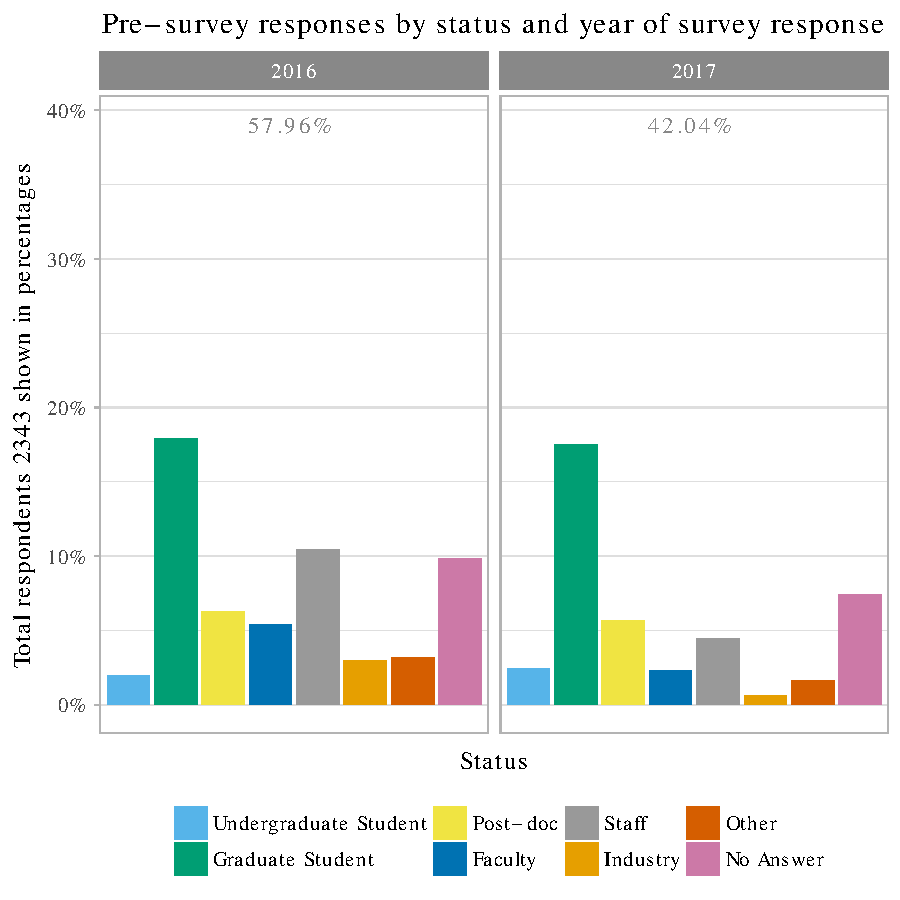
\includegraphics[width=.6\linewidth]{figure/calls-Rnwplotting-presurvey-data-1} 

}


\begin{kframe}\begin{alltt}
\hlkwd{plotByStatusGeneric}\hlstd{(Epreworkshop,} \hlstr{"Pre-survey"}\hlstd{,} \hlstr{"First.Time"} \hlstd{,} \hlstr{"first time taking a DC as learner"}\hlstd{,} \hlkwd{c}\hlstd{(}\hlnum{2}\hlstd{,}\hlnum{1}\hlstd{))}
\end{alltt}
\begin{verbatim}
## [1] 2343   34
## [1] "First.Time"
## [1] 2063   34
## 
##   No  Yes 
##  120 1943 
## [1] "Yes" "No"
\end{verbatim}
\end{kframe}

{\centering 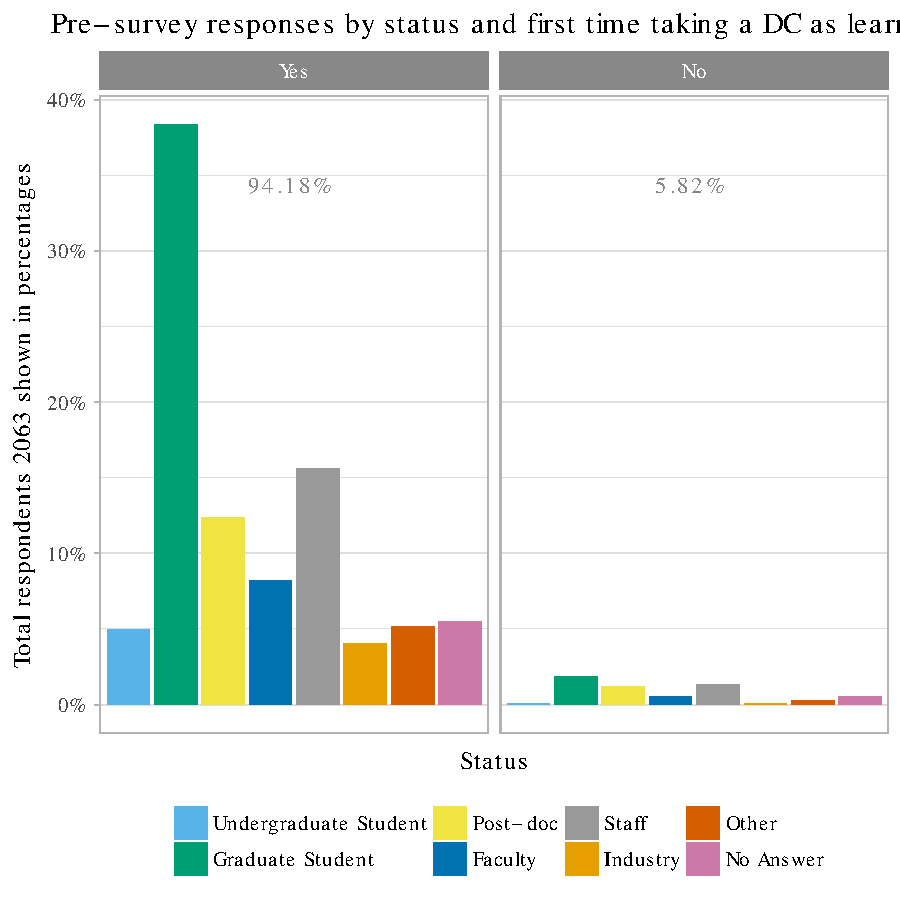
\includegraphics[width=.6\linewidth]{figure/calls-Rnwplotting-presurvey-data-2} 

}


\begin{kframe}\begin{alltt}
\hlcom{# table(Epreworkshop$Discipline) # too many variables to plot by Biology and Genetics is the discipline with the majority of answers}
\hlcom{# plotByStatusGeneric(Epreworkshop, "Pre-survey", "Discipline" , "discipline", c(2,10, 11,4,8,5,7,6, 9, 12,3, 14, 15, 16, 17,18, 13,1))}
\hlkwd{plotByStatusGeneric}\hlstd{(Epreworkshop,} \hlstr{"Pre-survey"}\hlstd{,} \hlstr{"OS"} \hlstd{,} \hlstr{"operative system"}\hlstd{,} \hlkwd{c}\hlstd{(}\hlnum{1}\hlstd{,}\hlnum{2}\hlstd{,}\hlnum{4}\hlstd{,}\hlnum{3}\hlstd{))}
\end{alltt}
\begin{verbatim}
## [1] 2343   34
## [1] "OS"
## [1] 1925   34
## 
## Apple OS    Linux Not sure  Windows 
##      769       67       53     1036 
## [1] "Apple OS" "Linux"    "Windows"  "Not sure"
\end{verbatim}
\end{kframe}

{\centering 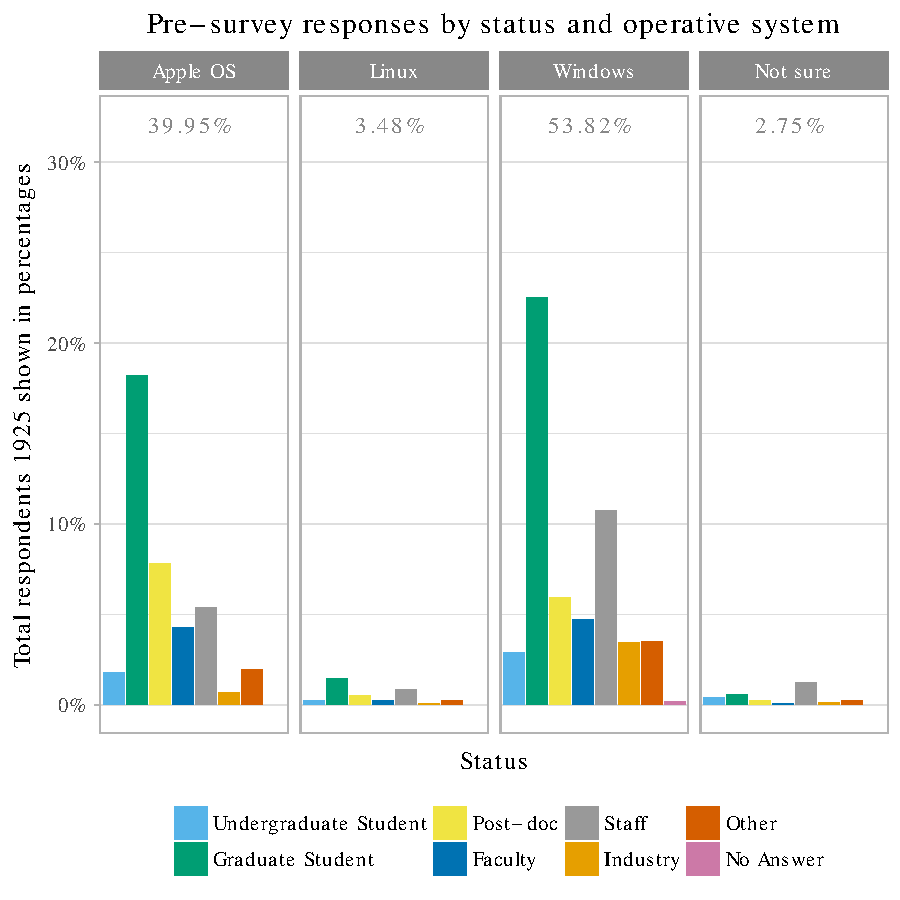
\includegraphics[width=.6\linewidth]{figure/calls-Rnwplotting-presurvey-data-3} 

}


\begin{kframe}\begin{alltt}
\hlcom{# table(Epreworkshop$With.Friend)}
\hlkwd{plotByStatusGeneric}\hlstd{(Epreworkshop,} \hlstr{"Pre-survey"}\hlstd{,} \hlstr{"With.Friend"} \hlstd{,} \hlstr{"attended with a friend"}\hlstd{,} \hlkwd{c}\hlstd{(}\hlnum{3}\hlstd{,}\hlnum{1}\hlstd{,}\hlnum{2}\hlstd{))}
\end{alltt}
\begin{verbatim}
## [1] 2343   34
## [1] "With.Friend"
## [1] 1922   34
## 
##       No Not sure      Yes 
##      620      375      927 
## [1] "Yes"      "No"       "Not sure"
\end{verbatim}
\end{kframe}

{\centering 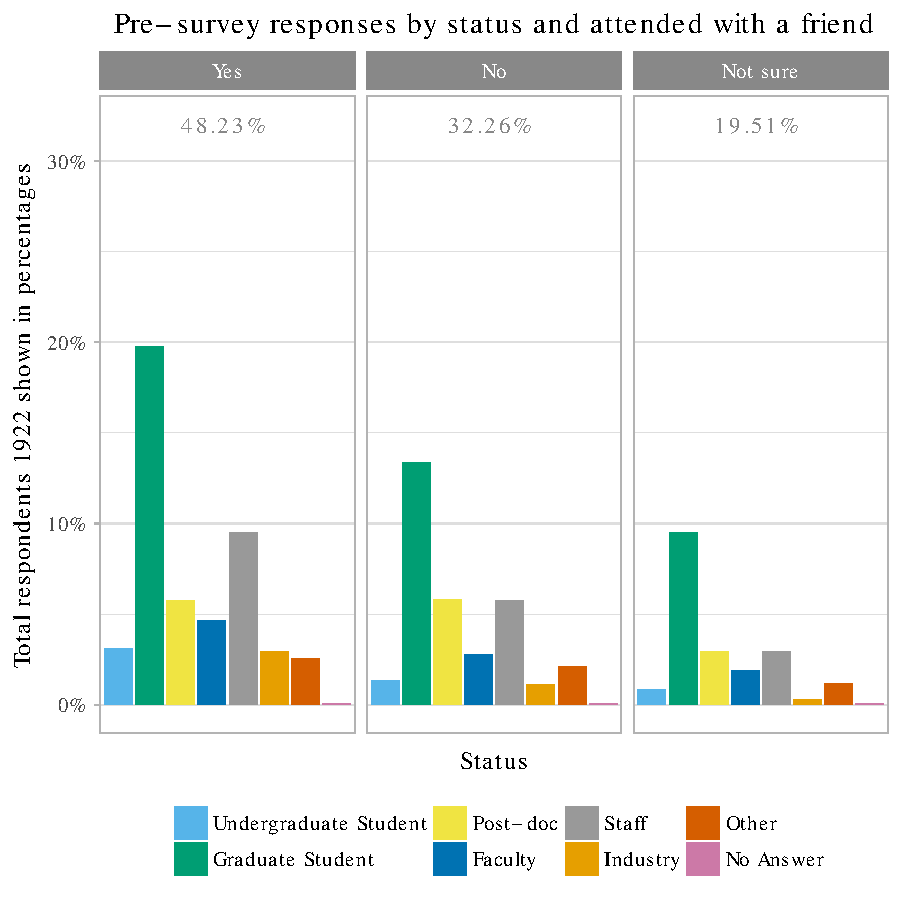
\includegraphics[width=.6\linewidth]{figure/calls-Rnwplotting-presurvey-data-4} 

}


\begin{kframe}\begin{alltt}
\hlcom{# table(Epreworkshop$Programming.Usage)}
\hlkwd{plotByStatusGeneric}\hlstd{(Epreworkshop,} \hlstr{"Pre-survey"}\hlstd{,} \hlstr{"Programming.Usage"} \hlstd{,} \hlstr{"programming usage"}\hlstd{,} \hlkwd{c}\hlstd{(}\hlnum{2}\hlstd{,} \hlnum{3}\hlstd{,} \hlnum{6}\hlstd{,} \hlnum{4}\hlstd{,} \hlnum{7}\hlstd{,} \hlnum{1}\hlstd{,} \hlnum{5}\hlstd{))}
\end{alltt}
\begin{verbatim}
## [1] 2343   34
## [1] "Programming.Usage"
## [1] 1871   34
## 
##                   Daily I have never programmed   Less than once a year 
##                     261                     501                     322 
##                 Monthly                Not sure    Several times a year 
##                     167                      34                     319 
##                  Weekly 
##                     267 
## [1] "I have never programmed" "Less than once a year"   "Several times a year"   
## [4] "Monthly"                 "Weekly"                  "Daily"                  
## [7] "Not sure"
\end{verbatim}
\end{kframe}

{\centering 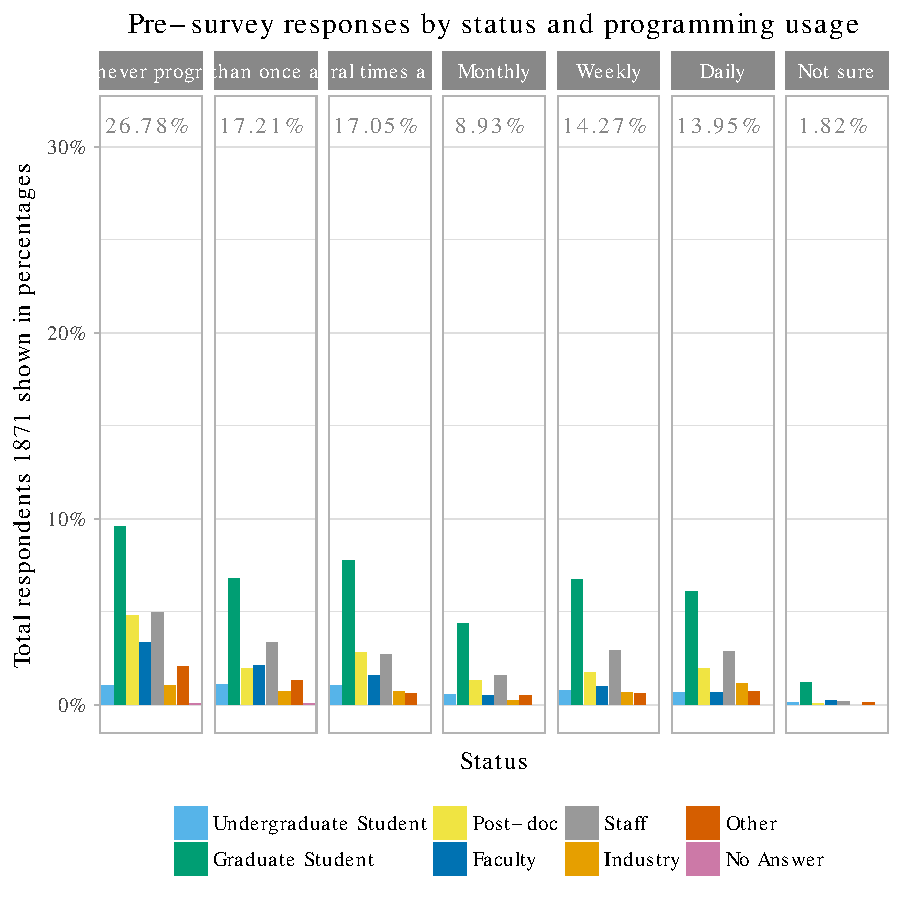
\includegraphics[width=.6\linewidth]{figure/calls-Rnwplotting-presurvey-data-5} 

}


\begin{kframe}\begin{alltt}
\hlcom{# Skipping current tools "Current.Tools.1" to "Current.Tools.7"}
\hlcom{# table(Epreworkshop$Have.Dataset)}
\hlkwd{plotByStatusGeneric}\hlstd{(Epreworkshop,} \hlstr{"Pre-survey"}\hlstd{,} \hlstr{"Have.Dataset"} \hlstd{,} \hlstr{"having a dataset"}\hlstd{,} \hlkwd{c}\hlstd{(}\hlnum{2}\hlstd{,}\hlnum{1}\hlstd{,}\hlnum{4}\hlstd{,}\hlnum{3}\hlstd{))}
\end{alltt}
\begin{verbatim}
## [1] 2343   34
## [1] "Have.Dataset"
## [1] 1859   34
## 
##              I am working on generating data                       I do not have data yet 
##                                          361                                          518 
##  I have data and done a fair bit of analysis I have data but haven't started analyzing it 
##                                          557                                          423 
## [1] "I do not have data yet"                      
## [2] "I am working on generating data"             
## [3] "I have data but haven't started analyzing it"
## [4] "I have data and done a fair bit of analysis"
\end{verbatim}
\end{kframe}

{\centering 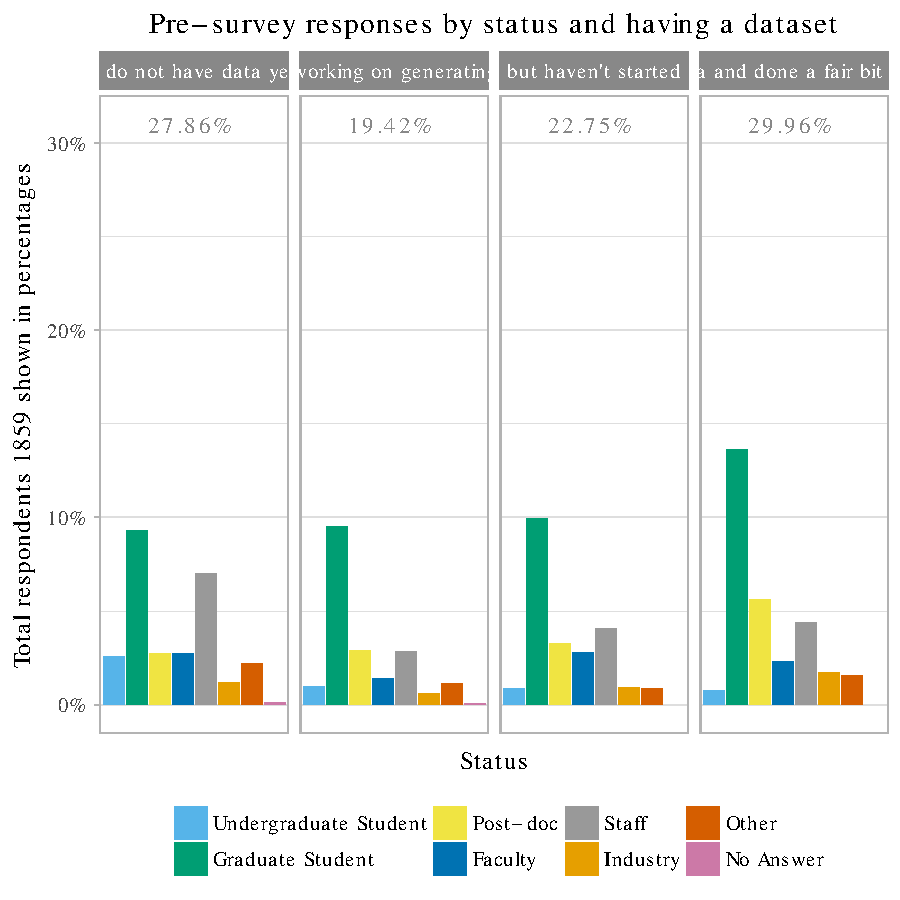
\includegraphics[width=.6\linewidth]{figure/calls-Rnwplotting-presurvey-data-6} 

}


\begin{kframe}\begin{alltt}
\hlcom{# "Data.Management.Strategy" "Data.Analysis.Workflow" are better plotted with a Likert plot }
\hlcom{# table(Epreworkshop$Data.Management.Strategy)}
\hlcom{# table(Epreworkshop$Data.Analysis.Workflow)}
\hlkwd{plotByStatusGeneric}\hlstd{(Epreworkshop,} \hlstr{"Pre-survey"}\hlstd{,} \hlstr{"Data.Organization"} \hlstd{,} \hlstr{"importance of data organization"}\hlstd{,} \hlkwd{c}\hlstd{(}\hlnum{4}\hlstd{,}\hlnum{1}\hlstd{,}\hlnum{3}\hlstd{,}\hlnum{2}\hlstd{,}\hlnum{5}\hlstd{))}
\end{alltt}
\begin{verbatim}
## [1] 2343   34
## [1] "Data.Organization"
## [1] 1852   34
## 
##             Agree          Disagree           Neutral    Strongly agree Strongly disagree 
##               590                 9                60              1135                58 
## [1] "Strongly agree"    "Agree"             "Neutral"           "Disagree"         
## [5] "Strongly disagree"
\end{verbatim}
\end{kframe}

{\centering 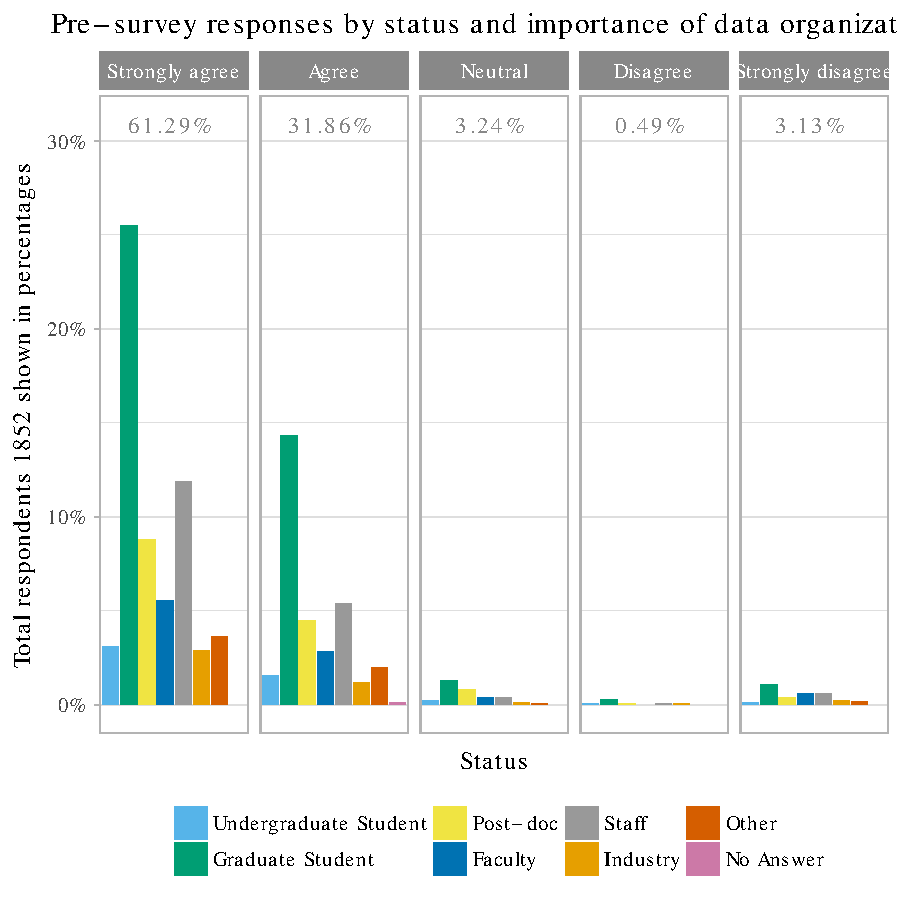
\includegraphics[width=.6\linewidth]{figure/calls-Rnwplotting-presurvey-data-7} 

}


\begin{kframe}\begin{alltt}
\hlcom{# table(Epreworkshop$Using.Scripting.Language)}
\hlkwd{plotByStatusGeneric}\hlstd{(Epreworkshop,} \hlstr{"Pre-survey"}\hlstd{,} \hlstr{"Using.Scripting.Language"} \hlstd{,} \hlstr{"importance of using a scripting language"}\hlstd{,}  \hlkwd{c}\hlstd{(}\hlnum{4}\hlstd{,}\hlnum{1}\hlstd{,}\hlnum{3}\hlstd{,}\hlnum{2}\hlstd{,}\hlnum{5}\hlstd{))}
\end{alltt}
\begin{verbatim}
## [1] 2343   34
## [1] "Using.Scripting.Language"
## [1] 1844   34
## 
##             Agree          Disagree           Neutral    Strongly agree Strongly disagree 
##               589                11               306               895                43 
## [1] "Strongly agree"    "Agree"             "Neutral"           "Disagree"         
## [5] "Strongly disagree"
\end{verbatim}
\end{kframe}

{\centering 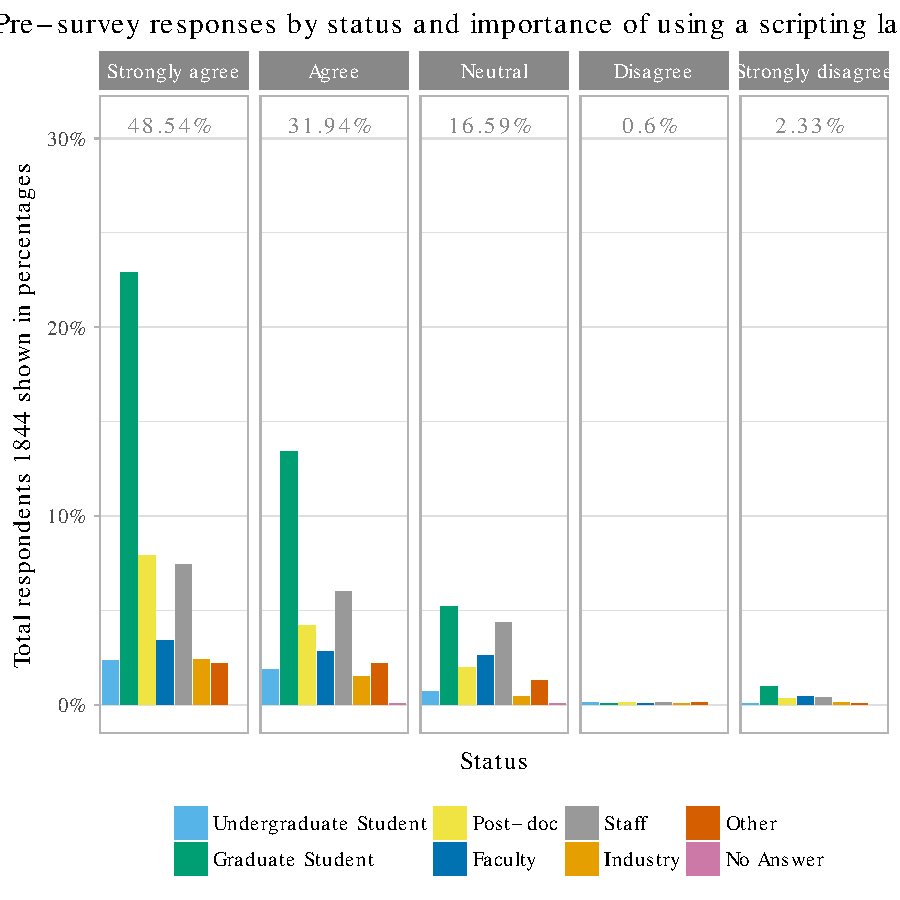
\includegraphics[width=.6\linewidth]{figure/calls-Rnwplotting-presurvey-data-8} 

}


\begin{kframe}\begin{alltt}
\hlcom{# ### Skipped because question is not clear}
\hlcom{# table(Epreworkshop$Using.R.or.Python)}
\hlcom{# table(Epreworkshop$Value.of.SQL.or.Python)}
\hlcom{# Taken in the US}
\hlcom{# table(Epreworkshop$Workshop.in.US)}
\hlcom{# 31% No 69% Yes}
\hlcom{#(590 * 100) / 1890  }
\hlcom{# ### [1] 31.21693}
\hlcom{#(1307 * 100) / 1890  }
\hlcom{# ###[1] 69.15344}
\hlkwd{plotByStatusGeneric}\hlstd{(Epreworkshop,} \hlstr{"Pre-survey"}\hlstd{,} \hlstr{"Workshop.in.US"} \hlstd{,} \hlstr{"workshop taken in the US"}\hlstd{)}
\end{alltt}
\begin{verbatim}
## [1] 2343   34
## [1] "Workshop.in.US"
## [1] 1897   34
## 
##   No  Yes 
##  590 1307
\end{verbatim}
\end{kframe}

{\centering 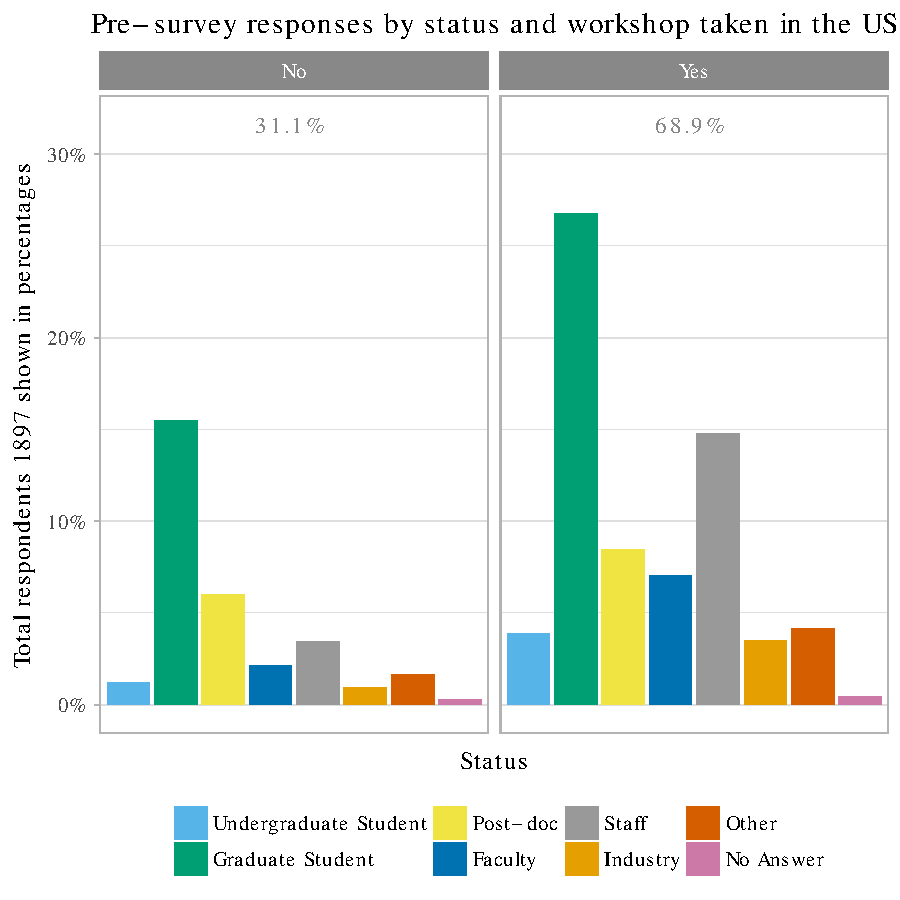
\includegraphics[width=.6\linewidth]{figure/calls-Rnwplotting-presurvey-data-9} 

}


\begin{kframe}\begin{alltt}
\hlcom{# make workshop in the US per year}
\hlkwd{plotGeneric}\hlstd{(Epreworkshop,} \hlstr{"Pre-survey"}\hlstd{,} \hlstr{"Workshop.in.US"} \hlstd{,} \hlstr{"workshop taken in the US per year"}\hlstd{,} \hlkwd{c}\hlstd{(}\hlnum{2}\hlstd{,}\hlnum{1}\hlstd{),} \hlstr{"year.survey"} \hlstd{)}
\end{alltt}
\begin{verbatim}
## [1] 2343   34
## [1] "Workshop.in.US"
## [1] "year.survey"
## [1] 1897   34
## [1] "Yes" "No" 
##      
##       2016 2017
##   Yes  706  601
##   No   393  197
\end{verbatim}
\end{kframe}

{\centering 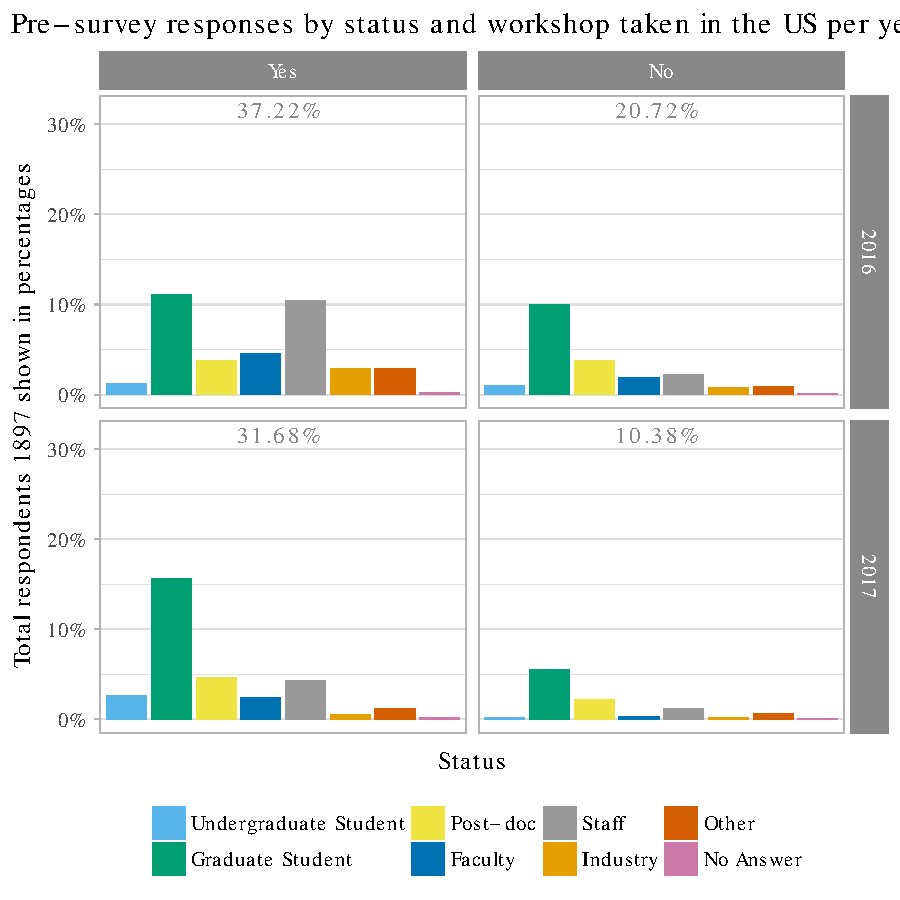
\includegraphics[width=.6\linewidth]{figure/calls-Rnwplotting-presurvey-data-10} 

}


\begin{kframe}\begin{alltt}
\hlcom{# this is very interesting, shows that for 2017 only 10% of respondents have taken the survey outside of the US}
\hlkwd{plotByStatusGeneric}\hlstd{(Epreworkshop,} \hlstr{"Pre-survey"}\hlstd{,} \hlstr{"Age"} \hlstd{,} \hlstr{"age"}\hlstd{)}
\end{alltt}
\begin{verbatim}
## [1] 2343   34
## [1] "Age"
## [1] 1279   34
## 
##             18-24             25-34             35-44             45-54             55-64 
##               210               579               250               133                72 
##             65-74 Prefer not to say 
##                12                23
\end{verbatim}
\end{kframe}

{\centering 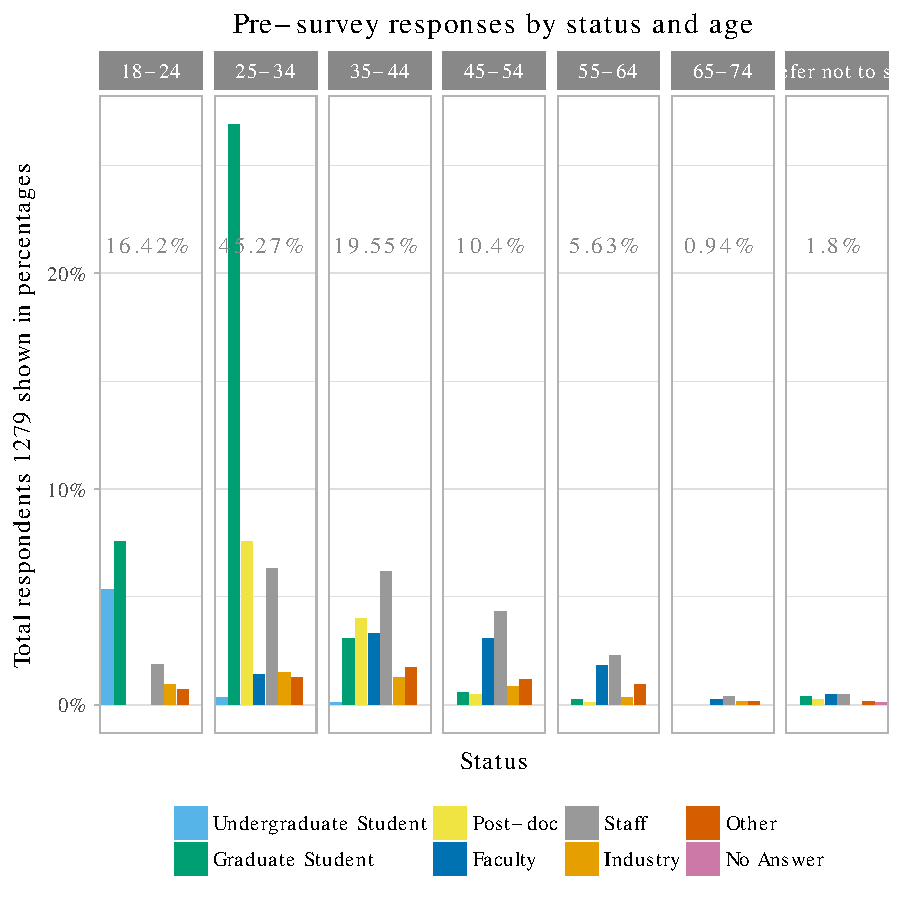
\includegraphics[width=.6\linewidth]{figure/calls-Rnwplotting-presurvey-data-11} 

}


\begin{kframe}\begin{alltt}
\hlkwd{plotGeneric}\hlstd{(Epreworkshop,} \hlstr{"Pre-survey"}\hlstd{,} \hlstr{"Age"} \hlstd{,} \hlstr{"age per year"}\hlstd{,}\hlkwa{NULL}\hlstd{,} \hlstr{"year.survey"}\hlstd{)}
\end{alltt}
\begin{verbatim}
## [1] 2343   34
## [1] "Age"
## [1] "year.survey"
## [1] 1279   34
##                    
##                     2016 2017
##   18-24               93  117
##   25-34              281  298
##   35-44              152   98
##   45-54               89   44
##   55-64               55   17
##   65-74                6    6
##   Prefer not to say   19    4
\end{verbatim}
\end{kframe}

{\centering 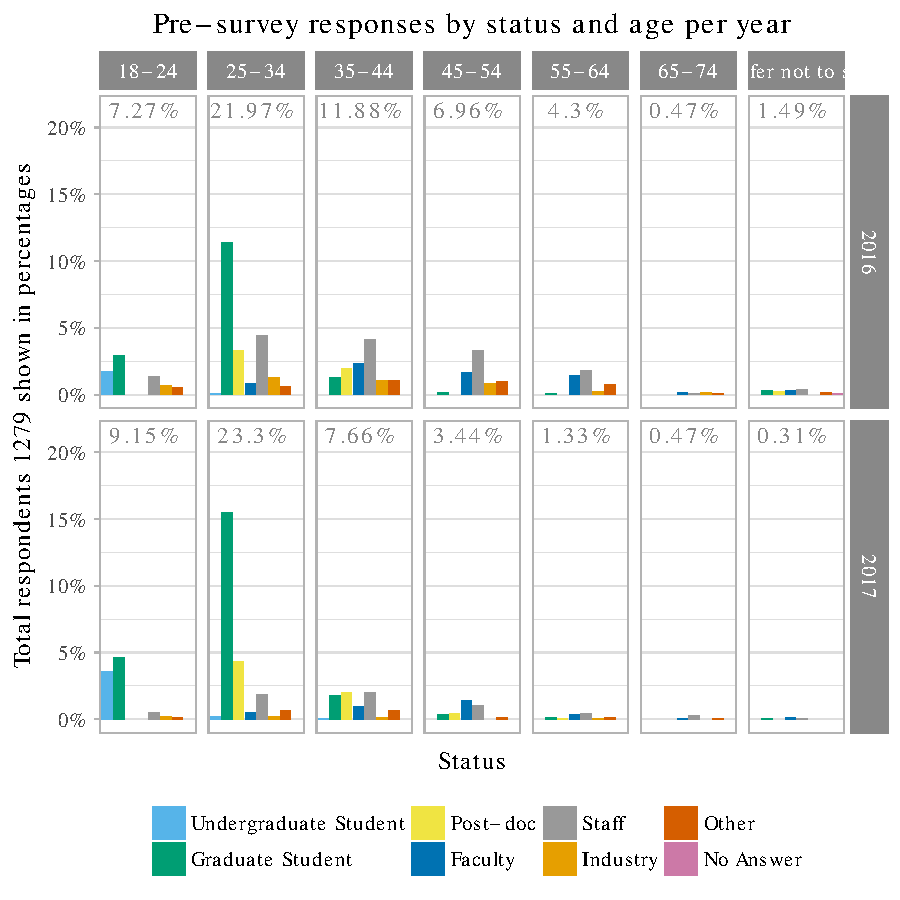
\includegraphics[width=.6\linewidth]{figure/calls-Rnwplotting-presurvey-data-12} 

}


\begin{kframe}\begin{alltt}
\hlcom{# doesn't really mean that more people in the US came with a friend, it just looks like that because more people}
\hlcom{# have taken the survey in the US}
\hlkwd{plotGeneric}\hlstd{(Epreworkshop,} \hlstr{"Pre-survey"}\hlstd{,}\hlstr{"With.Friend"} \hlstd{,} \hlstr{"came with friend vs taken in the US"}\hlstd{,} \hlkwd{c}\hlstd{(}\hlnum{3}\hlstd{,}\hlnum{1}\hlstd{,}\hlnum{2}\hlstd{),}
            \hlstr{"Workshop.in.US"} \hlstd{,} \hlkwd{c}\hlstd{(}\hlnum{2}\hlstd{,}\hlnum{1}\hlstd{))}
\end{alltt}
\begin{verbatim}
## [1] 2343   34
## [1] "With.Friend"
## [1] "Workshop.in.US"
## [1] 1869   34
## [1] "Yes"      "No"       "Not sure"
## [1] "Yes" "No" 
##           
##            Yes  No
##   Yes      604 296
##   No       415 187
##   Not sure 267 100
\end{verbatim}
\end{kframe}

{\centering 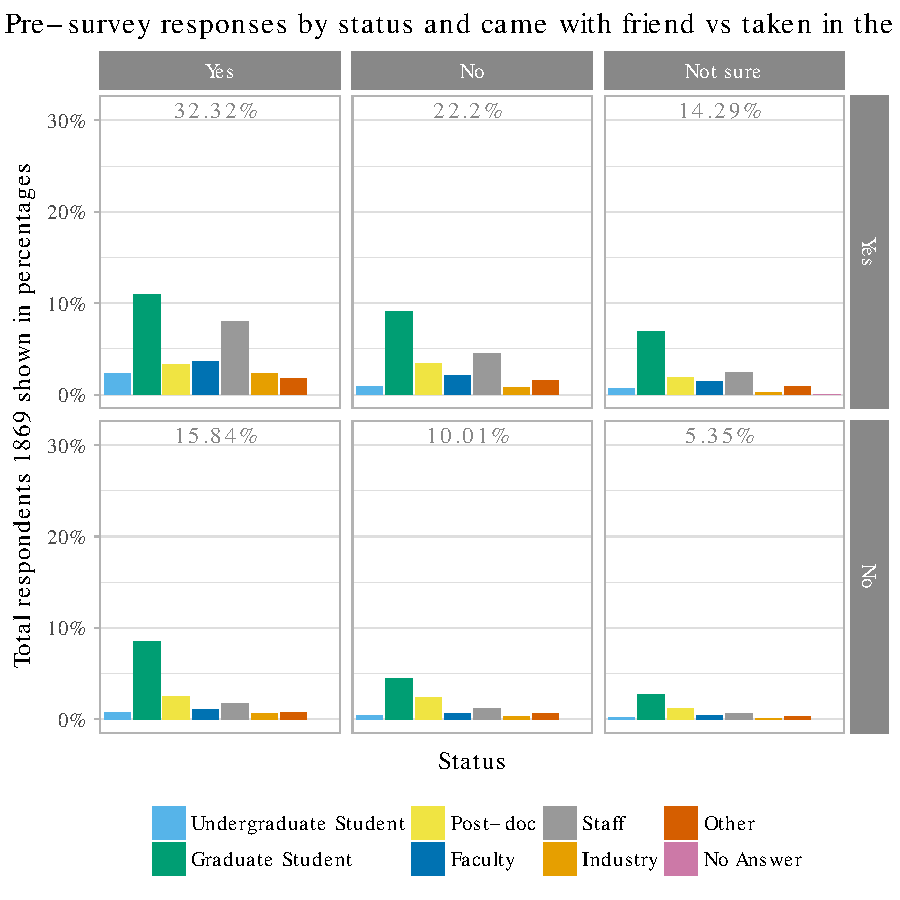
\includegraphics[width=.6\linewidth]{figure/calls-Rnwplotting-presurvey-data-13} 

}


\begin{kframe}\begin{alltt}
\hlkwd{plotGeneric}\hlstd{(Epreworkshop,} \hlstr{"Pre-survey"}\hlstd{,} \hlstr{"OS"}\hlstd{,} \hlstr{"OS vs taken in the US"}\hlstd{,} \hlkwd{c}\hlstd{(}\hlnum{1}\hlstd{,}\hlnum{2}\hlstd{,}\hlnum{4}\hlstd{,}\hlnum{3}\hlstd{),} \hlstr{"Workshop.in.US"} \hlstd{,} \hlkwd{c}\hlstd{(}\hlnum{2}\hlstd{,}\hlnum{1}\hlstd{))}
\end{alltt}
\begin{verbatim}
## [1] 2343   34
## [1] "OS"
## [1] "Workshop.in.US"
## [1] 1872   34
## [1] "Apple OS" "Linux"    "Windows"  "Not sure"
## [1] "Yes" "No" 
##           
##            Yes  No
##   Apple OS 542 207
##   Linux     41  24
##   Windows  668 338
##   Not sure  38  14
\end{verbatim}
\end{kframe}

{\centering 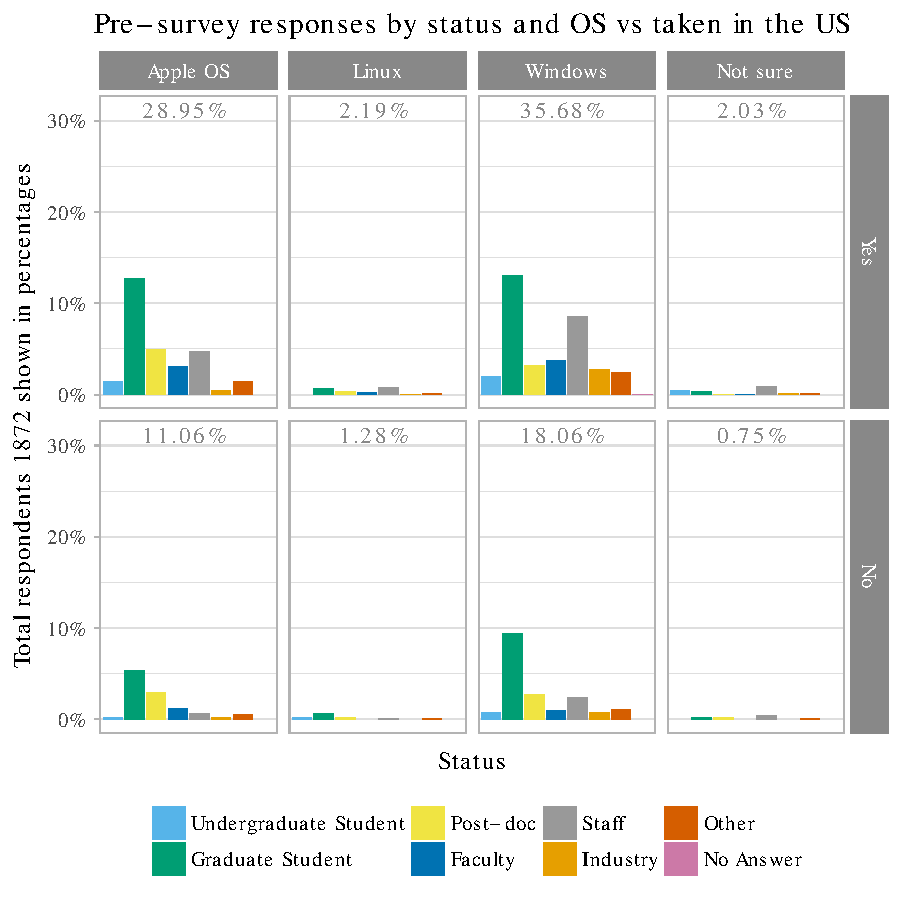
\includegraphics[width=.6\linewidth]{figure/calls-Rnwplotting-presurvey-data-14} 

}


\begin{kframe}\begin{alltt}
\hlkwd{plotGeneric}\hlstd{(Epreworkshop,} \hlstr{"Pre-survey"}\hlstd{,} \hlstr{"OS"}\hlstd{,} \hlstr{"OS vs year of the survey"}\hlstd{,} \hlkwd{c}\hlstd{(}\hlnum{1}\hlstd{,}\hlnum{2}\hlstd{,}\hlnum{4}\hlstd{,}\hlnum{3}\hlstd{),} \hlstr{"year.survey"} \hlstd{)}
\end{alltt}
\begin{verbatim}
## [1] 2343   34
## [1] "OS"
## [1] "year.survey"
## [1] 1925   34
## [1] "Apple OS" "Linux"    "Windows"  "Not sure"
##           
##            2016 2017
##   Apple OS  422  347
##   Linux      41   26
##   Windows   633  403
##   Not sure   25   28
\end{verbatim}
\end{kframe}

{\centering 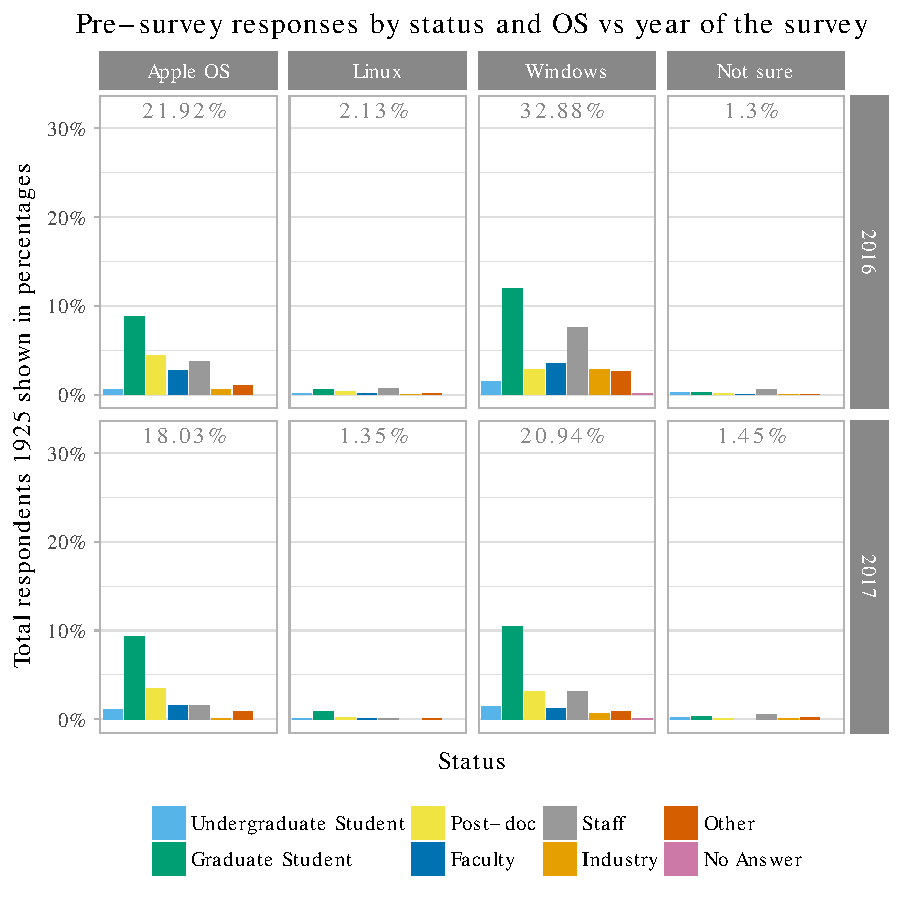
\includegraphics[width=.6\linewidth]{figure/calls-Rnwplotting-presurvey-data-15} 

}



\end{knitrout}
\begin{knitrout}
\definecolor{shadecolor}{rgb}{0.969, 0.969, 0.969}\color{fgcolor}\begin{kframe}
\begin{alltt}
\hlcom{# Filter all of those who did not take the survey in the US }
\hlstd{EpreworkshopUS} \hlkwb{<-} \hlkwd{subset}\hlstd{(Epreworkshop, Workshop.in.US} \hlopt{==} \hlstr{"Yes"}\hlstd{)}
\hlkwd{dim}\hlstd{(EpreworkshopUS)}
\end{alltt}
\begin{verbatim}
## [1] 1307   34
\end{verbatim}
\begin{alltt}
\hlkwd{plotByStatusGeneric}\hlstd{(EpreworkshopUS,} \hlstr{"Pre-surveyUS"}\hlstd{,} \hlstr{"Age"} \hlstd{,} \hlstr{"age"}\hlstd{)}
\end{alltt}
\begin{verbatim}
## [1] 1307   34
## [1] "Age"
## [1] 1279   34
## 
##             18-24             25-34             35-44             45-54             55-64 
##               210               579               250               133                72 
##             65-74 Prefer not to say 
##                12                23
\end{verbatim}
\end{kframe}

{\centering 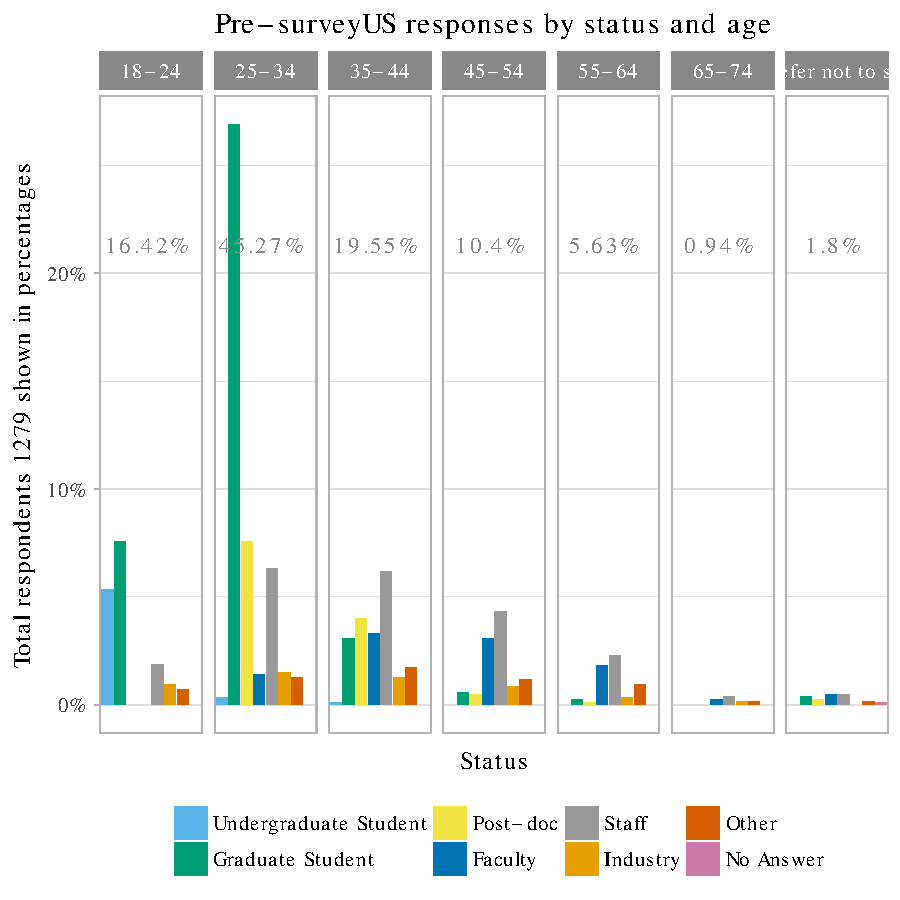
\includegraphics[width=.6\linewidth]{figure/calls-Rnwplotting-presurvey-dataUS-1} 

}


\begin{kframe}\begin{alltt}
\hlcom{# Gender... this is not a reality, it only means that more women responded in the survey}
\hlcom{# not that there were more women have taken the workshop}
\hlkwd{plotByStatusGeneric}\hlstd{(EpreworkshopUS,} \hlstr{"Pre-surveyUS"}\hlstd{,} \hlstr{"Gender"} \hlstd{,} \hlstr{"gender"}\hlstd{)}
\end{alltt}
\begin{verbatim}
## [1] 1307   34
## [1] "Gender"
## [1] 1307   34
## 
##            Female              Male Prefer not to say         No Answer 
##               717               540                22                28
\end{verbatim}
\end{kframe}

{\centering 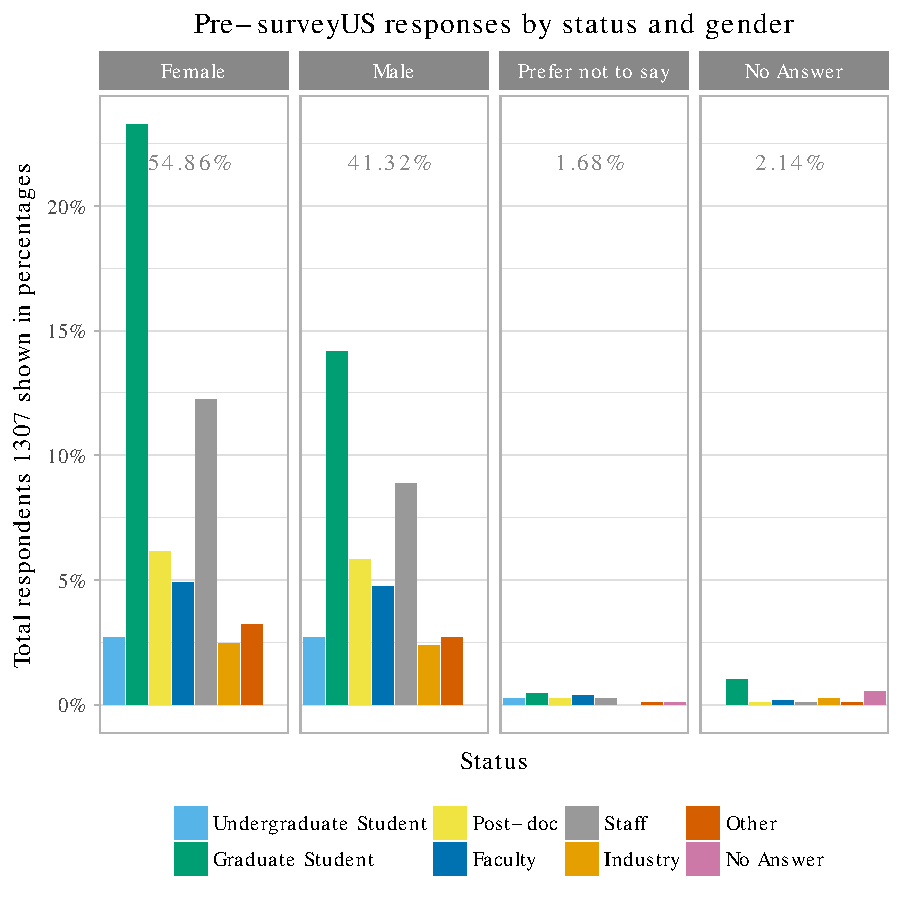
\includegraphics[width=.6\linewidth]{figure/calls-Rnwplotting-presurvey-dataUS-2} 

}


\begin{kframe}\begin{alltt}
\hlcom{# Combined plot}
\hlkwd{plotGeneric}\hlstd{(EpreworkshopUS,} \hlstr{"Pre-surveyUS"}\hlstd{,}\hlstr{"With.Friend"} \hlstd{,} \hlstr{"came with friend vs gender"}\hlstd{,} \hlkwd{c}\hlstd{(}\hlnum{3}\hlstd{,}\hlnum{1}\hlstd{,}\hlnum{2}\hlstd{),}
            \hlstr{"Gender"} \hlstd{)}
\end{alltt}
\begin{verbatim}
## [1] 1307   34
## [1] "With.Friend"
## [1] "Gender"
## [1] 1286   34
## [1] "Yes"      "No"       "Not sure"
##           
##            Female Male Prefer not to say No Answer
##   Yes         329  257                10         8
##   No          234  173                 6         2
##   Not sure    148  110                 6         3
\end{verbatim}
\end{kframe}

{\centering 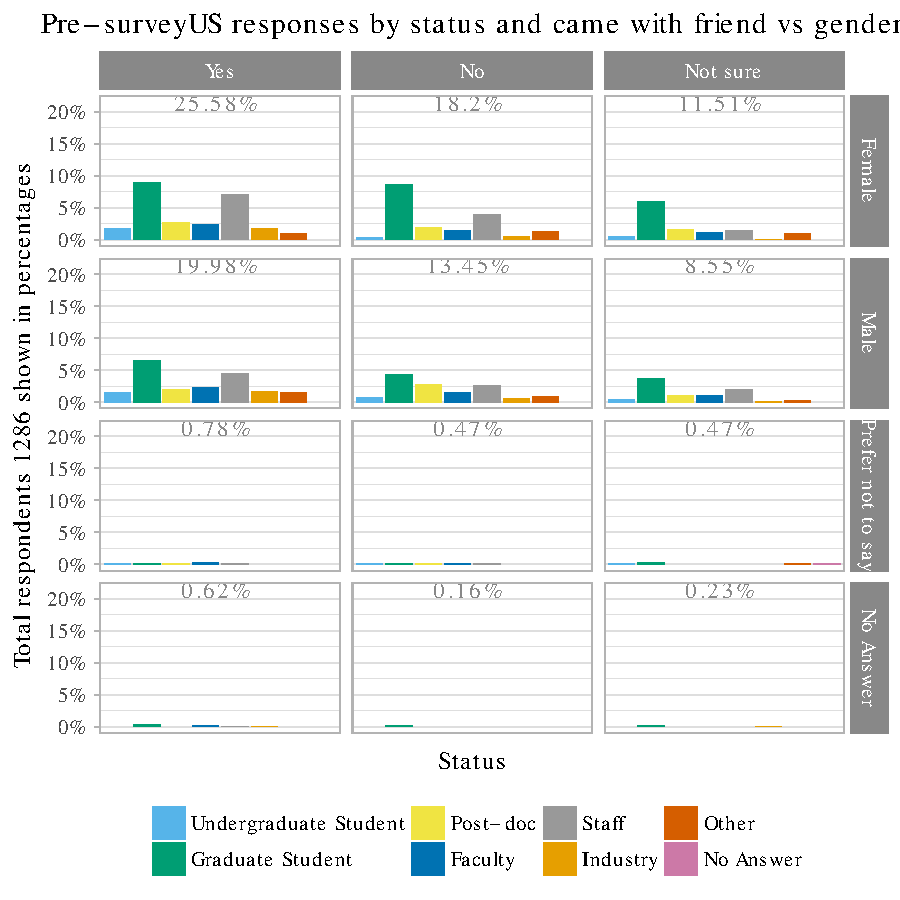
\includegraphics[width=.6\linewidth]{figure/calls-Rnwplotting-presurvey-dataUS-3} 

}


\begin{kframe}\begin{alltt}
\hlcom{# Names are too long to be shown in categories }
\hlkwd{plotByStatusGeneric}\hlstd{(EpreworkshopUS,} \hlstr{"Pre-surveyUS"}\hlstd{,} \hlstr{"Race"} \hlstd{,} \hlstr{"race"}\hlstd{)}
\end{alltt}
\begin{verbatim}
## [1] 1307   34
## [1] "Race"
## [1] 1307   34
## 
##         American Indian or Alaskan Native                  Asian / Pacific Islander 
##                                         2                                       290 
##                 Black or African American                        Hispanic or Latino 
##                                        56                                        57 
## Native Hawaiian or Other Pacific Islander                         White / Caucasian 
##                                         1                                       735 
##                         Prefer not to say                                     Other 
##                                        81                                        42 
##                                 No Answer 
##                                        43
\end{verbatim}
\end{kframe}

{\centering 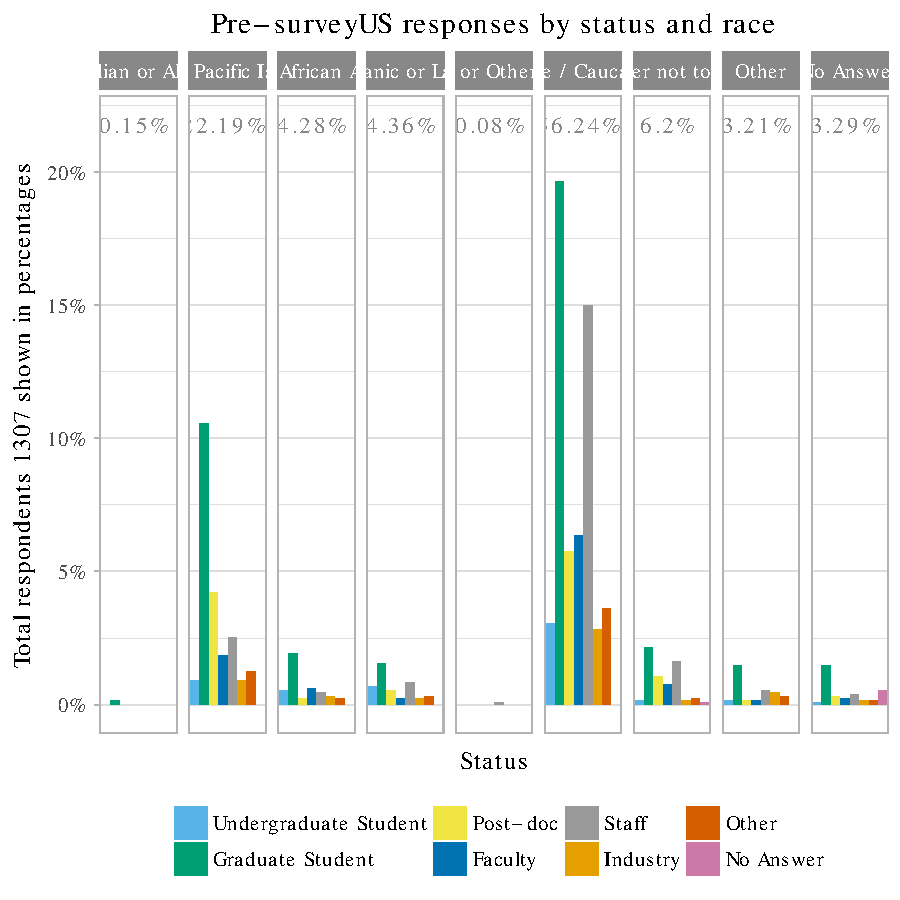
\includegraphics[width=.6\linewidth]{figure/calls-Rnwplotting-presurvey-dataUS-4} 

}


\begin{kframe}\begin{alltt}
\hlcom{# ############################################################################}
\end{alltt}
\end{kframe}
\end{knitrout}
\begin{knitrout}
\definecolor{shadecolor}{rgb}{0.969, 0.969, 0.969}\color{fgcolor}\begin{kframe}
\begin{alltt}
\hlstd{Epostworkshop} \hlkwb{<-} \hlkwd{Exploring}\hlstd{(}\hlstr{"data/postworkshop_public_archived.csv"}\hlstd{)}
\end{alltt}
\begin{verbatim}
## [1] "data/postworkshop_public_archived.csv"
## [1] "Data contains 1081 rows and 43 columns"
\end{verbatim}
\begin{alltt}
\hlstd{Epostworkshop} \hlkwb{<-} \hlkwd{cleanPostworkshopdata}\hlstd{(Epostworkshop)}
\end{alltt}
\begin{verbatim}
## [1] 1081   43
##  [1] "Start.Date"                "End.Date"                  "When.Taking.Survey"       
##  [4] "First.Time"                "Research"                  "Status"                   
##  [7] "Status.Other"              "Involvement"               "Practical.Knowledge"      
## [10] "Organize.Data"             "Use.OpenRefine"            "Import.Python"            
## [13] "Import.R"                  "Visualizations.in.Python"  "Visualizations.in.R"      
## [16] "Construct.SQL"             "Use.command.line"          "Skill.Level.Prior"        
## [19] "Skill.Level.Following"     "Data.Organization"         "Using.Scripting.Language" 
## [22] "Using.R.or.Python"         "Value.of.SQL.or.Python"    "Application"              
## [25] "Worth.My.Time"             "Material"                  "Recommend"                
## [28] "Instructors.Clear.Answers" "Instructors.Considerate"   "Instructors.Effective"    
## [31] "Instructors.Enthusiastic"  "Workshop.in.US"            "Age"                      
## [34] "Gender"                    "Gender.Other"              "Race.American.Indian"     
## [37] "Race.Asian"                "Race.Black"                "Race.Hispanic"            
## [40] "Race.Islander"             "Race.White"                "Race.Prefer.Not"          
## [43] "Race.Other"               
## [1] "Undergraduate Student" "Graduate student"      "Post-doc"             
## [4] "Faculty"               "Staff"                 "Industry"             
## [7] "Other"                 "No Answer"            
## [1] "Female"            "Male"              "Prefer not to say" "No Answer"        
## [1] "Data contains 1081 rows and 44 columns"
\end{verbatim}
\begin{alltt}
\hlcom{# Postworkshop has about half the entries in comparison with the preworkshop }
\end{alltt}
\end{kframe}
\end{knitrout}
\begin{knitrout}
\definecolor{shadecolor}{rgb}{0.969, 0.969, 0.969}\color{fgcolor}\begin{kframe}
\begin{alltt}
\hlcom{# 2017 has of course less entries because it contains only answers of half a year}
\hlkwd{plotByStatusGeneric}\hlstd{(Epostworkshop,} \hlstr{"Post-survey"}\hlstd{,} \hlstr{"year.survey"} \hlstd{,} \hlstr{"year of survey response"}\hlstd{)}
\end{alltt}
\begin{verbatim}
## [1] 1081   44
## [1] "year.survey"
## [1] 1080   44
## 
## 2016 2017 
##  602  478
\end{verbatim}
\end{kframe}

{\centering 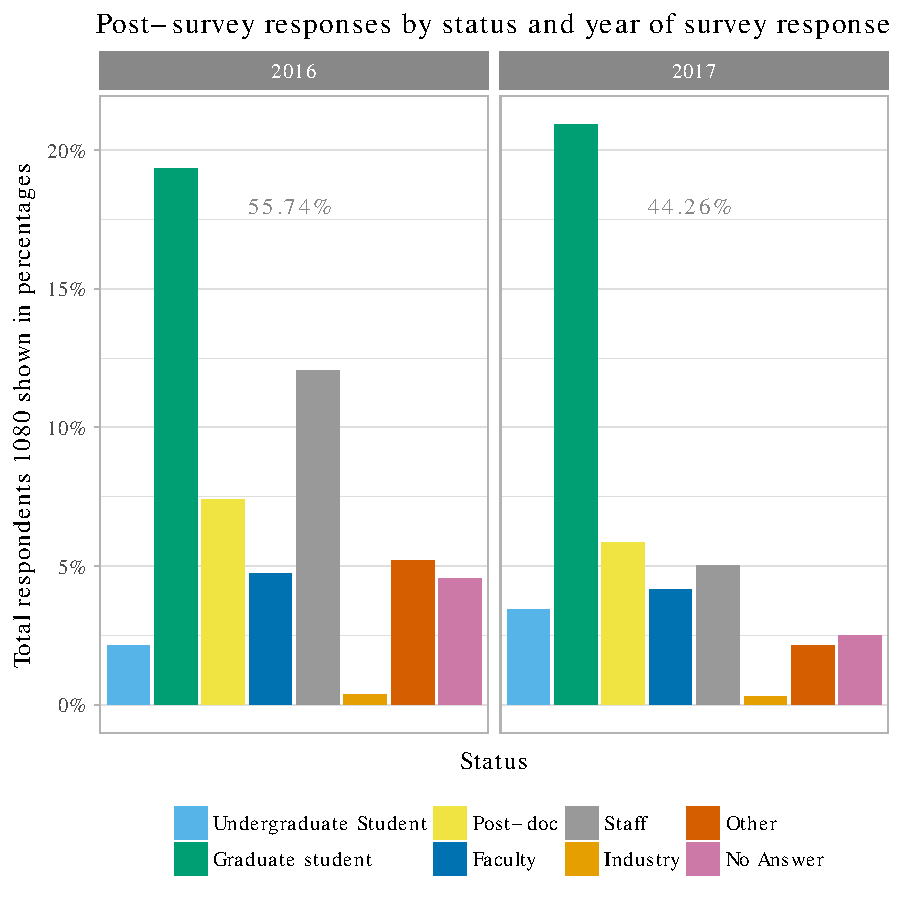
\includegraphics[width=.6\linewidth]{figure/calls-Rnwplotting-postsurvey-data-1} 

}


\begin{kframe}\begin{alltt}
\hlcom{# there is not much to do with columns that are repeated with the pre-survey}
\hlcom{# #  "When.Taking.Survey"        "First.Time"}
\hlcom{# # "Research" is a text field wich is difficult to categorize}
\hlcom{# table(Epostworkshop$Involvement)}
\hlkwd{plotByStatusGeneric}\hlstd{(Epostworkshop,} \hlstr{"Post-survey"}\hlstd{,} \hlstr{"Involvement"} \hlstd{,} \hlstr{"level of involvement"}\hlstd{,} \hlkwd{c}\hlstd{(}\hlnum{3}\hlstd{,}\hlnum{1}\hlstd{,}\hlnum{2}\hlstd{))}
\end{alltt}
\begin{verbatim}
## [1] 1081   44
## [1] "Involvement"
## [1] 1008   44
## 
## Enthusiastically involved         Somewhat involved             Very involved 
##                       347                       149                       512 
## [1] "Very involved"             "Enthusiastically involved" "Somewhat involved"
\end{verbatim}
\end{kframe}

{\centering 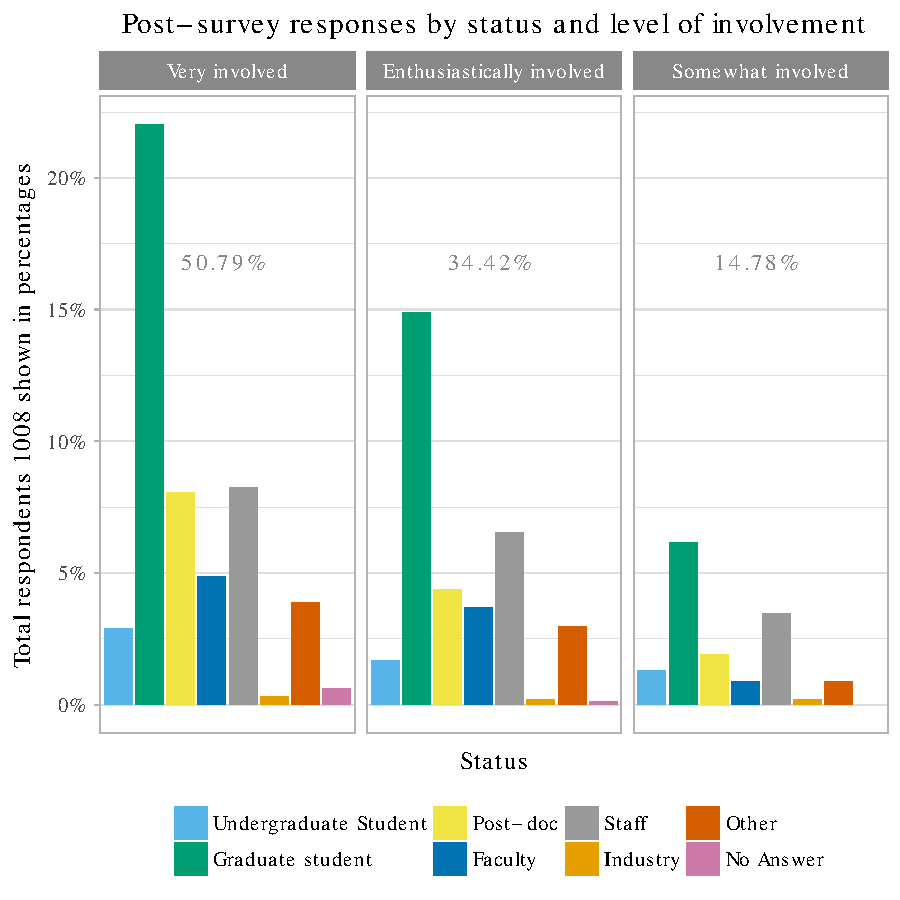
\includegraphics[width=.6\linewidth]{figure/calls-Rnwplotting-postsurvey-data-2} 

}


\begin{kframe}\begin{alltt}
\hlcom{# table(Epostworkshop$Practical.Knowledge)}
\hlkwd{plotByStatusGeneric}\hlstd{(Epostworkshop,} \hlstr{"Post-survey"}\hlstd{,} \hlstr{"Practical.Knowledge"} \hlstd{,} \hlstr{"practical knowledge gained"}\hlstd{,} \hlkwd{c}\hlstd{(}\hlnum{1}\hlstd{,} \hlnum{3}\hlstd{,} \hlnum{2}\hlstd{))}
\end{alltt}
\begin{verbatim}
## [1] 1081   44
## [1] "Practical.Knowledge"
## [1] 1009   44
## 
##             A great deal                     None Some practical knowledge 
##                      585                        6                      418 
## [1] "A great deal"             "Some practical knowledge" "None"
\end{verbatim}
\end{kframe}

{\centering 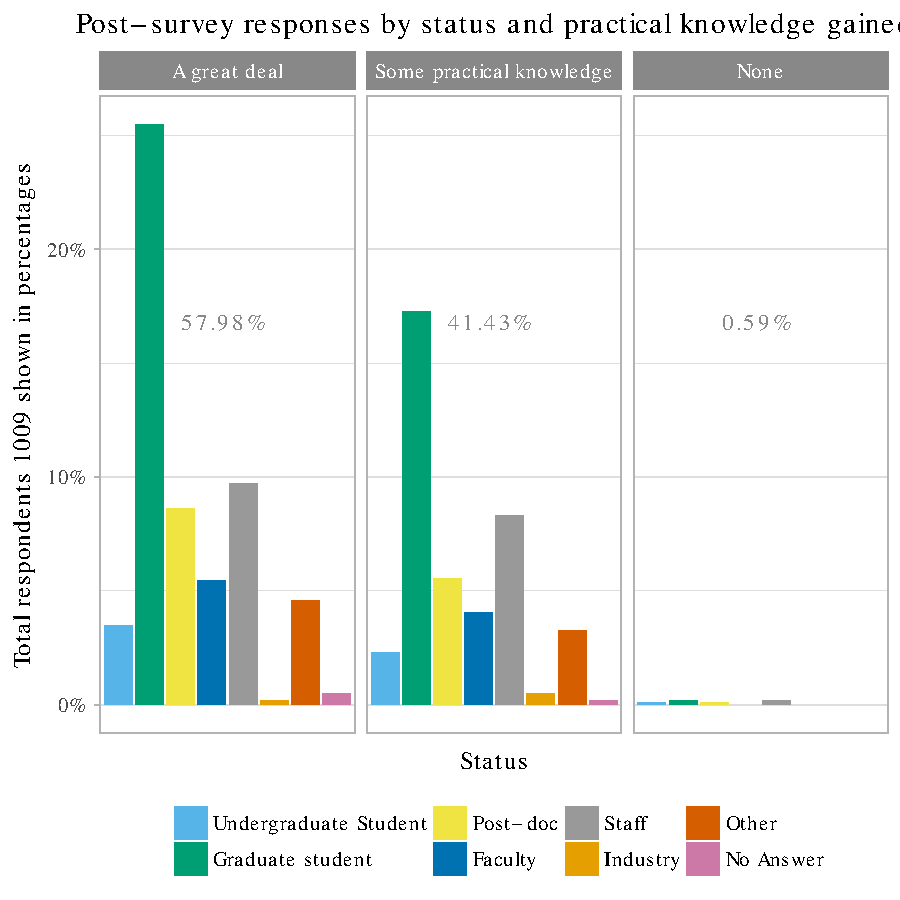
\includegraphics[width=.6\linewidth]{figure/calls-Rnwplotting-postsurvey-data-3} 

}


\begin{kframe}\begin{alltt}
\hlkwd{plotGeneric}\hlstd{(Epostworkshop,} \hlstr{"Post-survey"}\hlstd{,} \hlstr{"Practical.Knowledge"} \hlstd{,}
            \hlstr{"practical knowledge gained vs level of involvement"}\hlstd{,} \hlkwd{c}\hlstd{(}\hlnum{1}\hlstd{,} \hlnum{3}\hlstd{,} \hlnum{2}\hlstd{),}\hlstr{"Involvement"}\hlstd{,} \hlkwd{c}\hlstd{(}\hlnum{3}\hlstd{,}\hlnum{1}\hlstd{,}\hlnum{2}\hlstd{))}
\end{alltt}
\begin{verbatim}
## [1] 1081   44
## [1] "Practical.Knowledge"
## [1] "Involvement"
## [1] 1007   44
## [1] "A great deal"             "Some practical knowledge" "None"                    
## [1] "Very involved"             "Enthusiastically involved" "Somewhat involved"        
##                           
##                            Very involved Enthusiastically involved Somewhat involved
##   A great deal                       267                       267                50
##   Some practical knowledge           245                        79                93
##   None                                 0                         0                 6
\end{verbatim}
\end{kframe}

{\centering 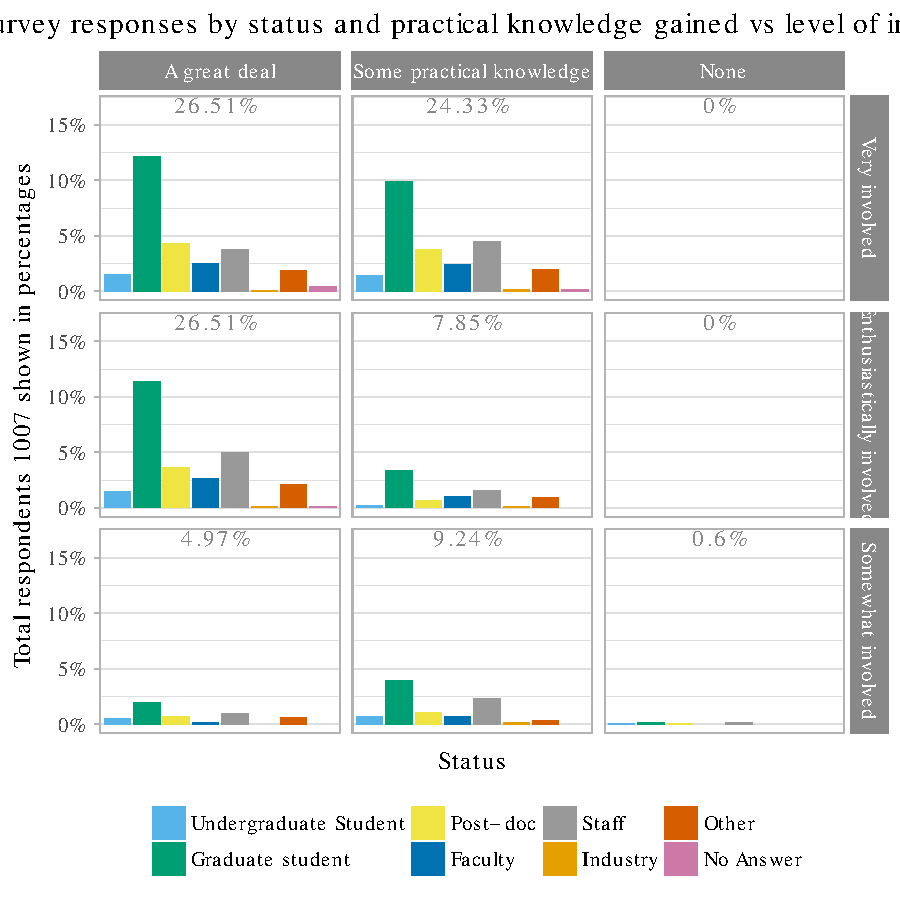
\includegraphics[width=.6\linewidth]{figure/calls-Rnwplotting-postsurvey-data-4} 

}


\begin{kframe}\begin{alltt}
\hlcom{# #####The folowwing will be better with a Likert plot}
\hlcom{# # "Organize.Data"             "Use.OpenRefine"            "Import.Python"            }
\hlcom{# # [13] "Import.R"                  "Visualizations.in.Python"  "Visualizations.in.R"       "Construct.SQL"            }
\hlcom{# # [17] "Use.command.line" }
\hlcom{# # For information of each question}
\hlcom{# table(Epostworkshop$Organize.Data)}
\hlkwd{plotByStatusGeneric}\hlstd{(Epostworkshop,} \hlstr{"Post-survey"}\hlstd{,} \hlstr{"Organize.Data"} \hlstd{,} \hlstr{"better understanding on how to organize data in spreadsheets"}\hlstd{,} \hlkwd{c}\hlstd{(}\hlnum{5}\hlstd{,}\hlnum{1}\hlstd{,}\hlnum{4}\hlstd{,}\hlnum{2}\hlstd{,}\hlnum{6}\hlstd{,}\hlnum{3}\hlstd{))}
\end{alltt}
\begin{verbatim}
## [1] 1081   44
## [1] "Organize.Data"
## [1] 965  44
## 
##                           Agree                        Disagree 
##                             362                              28 
## NA/Not covered at this workshop                         Neutral 
##                              81                             161 
##                  Strongly Agree               Strongly Disagree 
##                             311                              22 
## [1] "Strongly Agree"                  "Agree"                          
## [3] "Neutral"                         "Disagree"                       
## [5] "Strongly Disagree"               "NA/Not covered at this workshop"
\end{verbatim}
\end{kframe}

{\centering 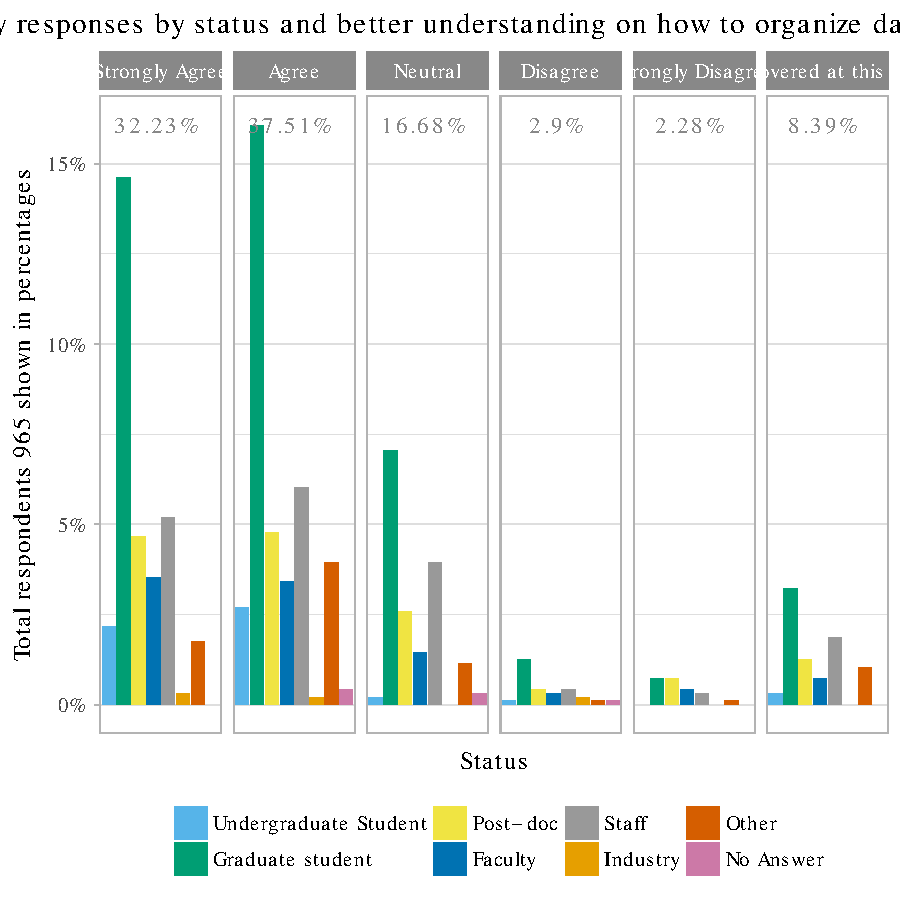
\includegraphics[width=.6\linewidth]{figure/calls-Rnwplotting-postsurvey-data-5} 

}


\begin{kframe}\begin{alltt}
\hlcom{# table(Epostworkshop$Use.OpenRefine)}
\hlkwd{plotByStatusGeneric}\hlstd{(Epostworkshop,} \hlstr{"Post-survey"}\hlstd{,} \hlstr{"Use.OpenRefine"} \hlstd{,} \hlstr{"better understanding on how to use OpenRefine for data cleaning"}\hlstd{,} \hlkwd{c}\hlstd{(}\hlnum{5}\hlstd{,}\hlnum{1}\hlstd{,}\hlnum{4}\hlstd{,}\hlnum{2}\hlstd{,}\hlnum{6}\hlstd{,}\hlnum{3}\hlstd{))}
\end{alltt}
\begin{verbatim}
## [1] 1081   44
## [1] "Use.OpenRefine"
## [1] 960  44
## 
##                           Agree                        Disagree 
##                             247                              31 
## NA/Not covered at this workshop                         Neutral 
##                             215                              85 
##                  Strongly Agree               Strongly disagree 
##                             351                              31 
## [1] "Strongly Agree"                  "Agree"                          
## [3] "Neutral"                         "Disagree"                       
## [5] "Strongly disagree"               "NA/Not covered at this workshop"
\end{verbatim}
\end{kframe}

{\centering 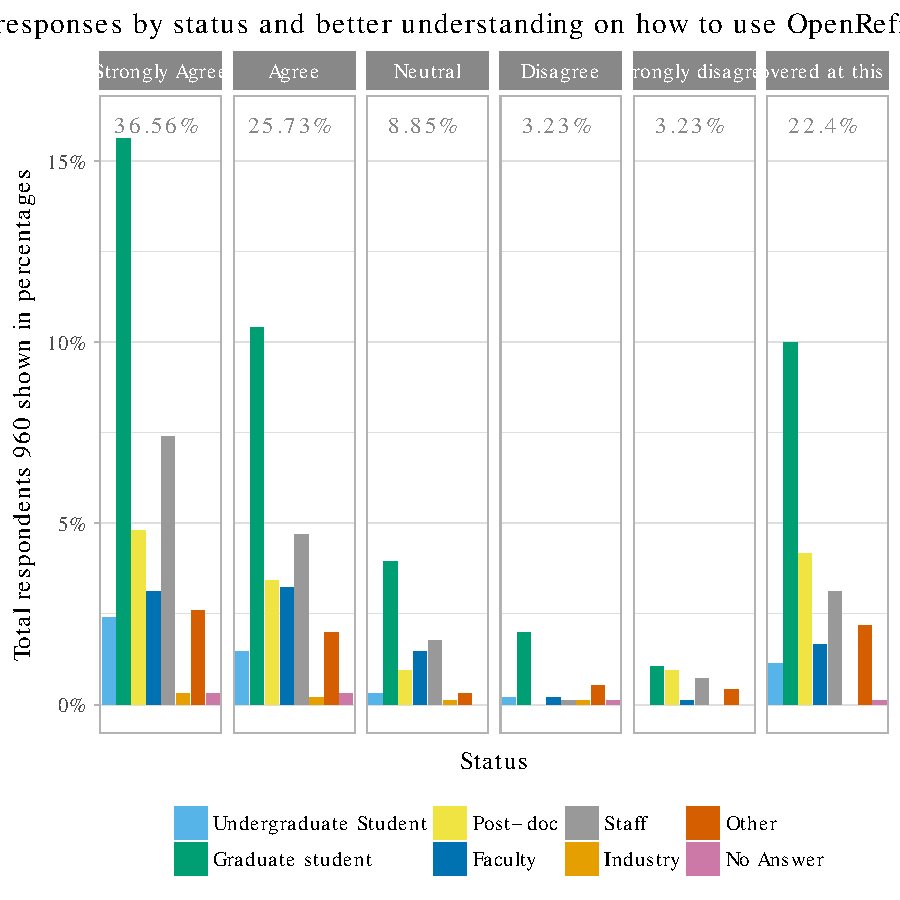
\includegraphics[width=.6\linewidth]{figure/calls-Rnwplotting-postsurvey-data-6} 

}


\begin{kframe}\begin{alltt}
\hlcom{# table(Epostworkshop$Import.Python)}
\hlcom{# it seems like half of the workshops did not cover python }
\hlkwd{plotByStatusGeneric}\hlstd{(Epostworkshop,} \hlstr{"Post-survey"}\hlstd{,} \hlstr{"Import.Python"} \hlstd{,} \hlstr{"better understanding on how to import a file in Python and work with the data"}\hlstd{,}  \hlkwd{c}\hlstd{(}\hlnum{5}\hlstd{,}\hlnum{1}\hlstd{,}\hlnum{4}\hlstd{,}\hlnum{2}\hlstd{,}\hlnum{6}\hlstd{,}\hlnum{3}\hlstd{))}
\end{alltt}
\begin{verbatim}
## [1] 1081   44
## [1] "Import.Python"
## [1] 954  44
## 
##                           Agree                        Disagree 
##                             107                              70 
## NA/Not covered at this workshop                         Neutral 
##                             521                              96 
##                  Strongly Agree               Strongly disagree 
##                              97                              63 
## [1] "Strongly Agree"                  "Agree"                          
## [3] "Neutral"                         "Disagree"                       
## [5] "Strongly disagree"               "NA/Not covered at this workshop"
\end{verbatim}
\end{kframe}

{\centering 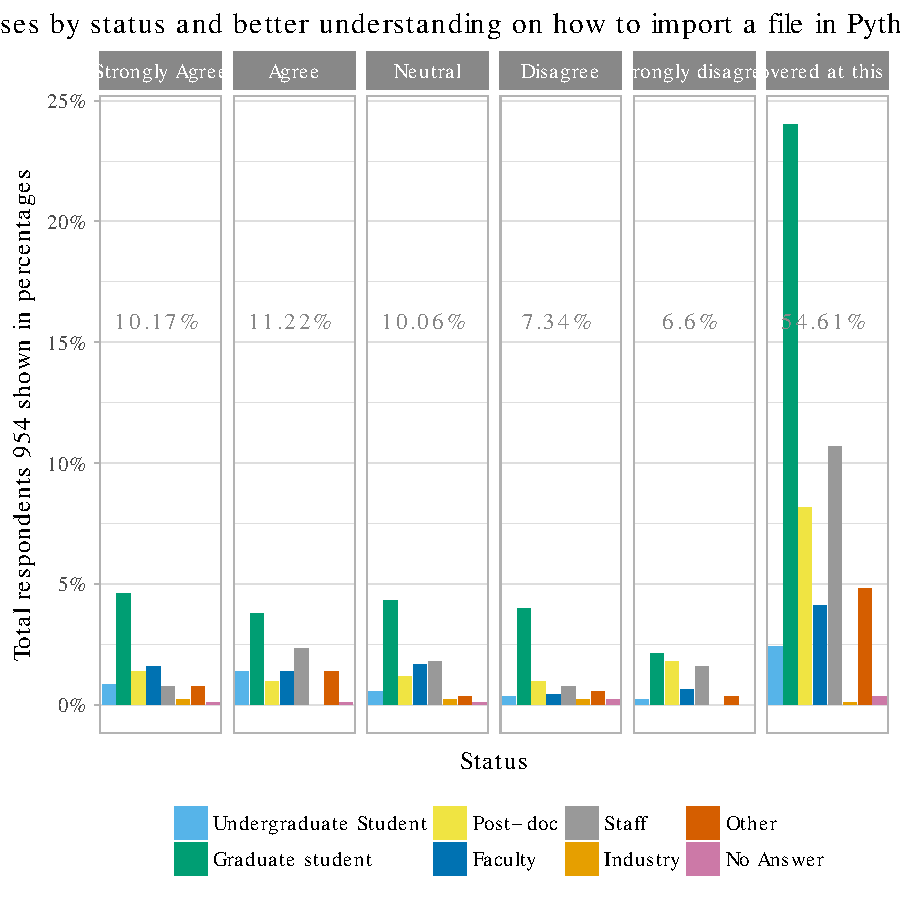
\includegraphics[width=.6\linewidth]{figure/calls-Rnwplotting-postsurvey-data-7} 

}


\begin{kframe}\begin{alltt}
\hlcom{# table(Epostworkshop$Visualizations.in.Python)}
\hlkwd{plotByStatusGeneric}\hlstd{(Epostworkshop,} \hlstr{"Post-survey"}\hlstd{,} \hlstr{"Visualizations.in.Python"} \hlstd{,} \hlstr{"better understanding on how to do visualizations in Python"}\hlstd{,}  \hlkwd{c}\hlstd{(}\hlnum{5}\hlstd{,}\hlnum{1}\hlstd{,}\hlnum{4}\hlstd{,}\hlnum{2}\hlstd{,}\hlnum{6}\hlstd{,}\hlnum{3}\hlstd{))}
\end{alltt}
\begin{verbatim}
## [1] 1081   44
## [1] "Visualizations.in.Python"
## [1] 958  44
## 
##                           Agree                        Disagree 
##                             108                              78 
## NA/Not covered at this workshop                         Neutral 
##                             526                             105 
##                  Strongly Agree               Strongly disagree 
##                              76                              65 
## [1] "Strongly Agree"                  "Agree"                          
## [3] "Neutral"                         "Disagree"                       
## [5] "Strongly disagree"               "NA/Not covered at this workshop"
\end{verbatim}
\end{kframe}

{\centering 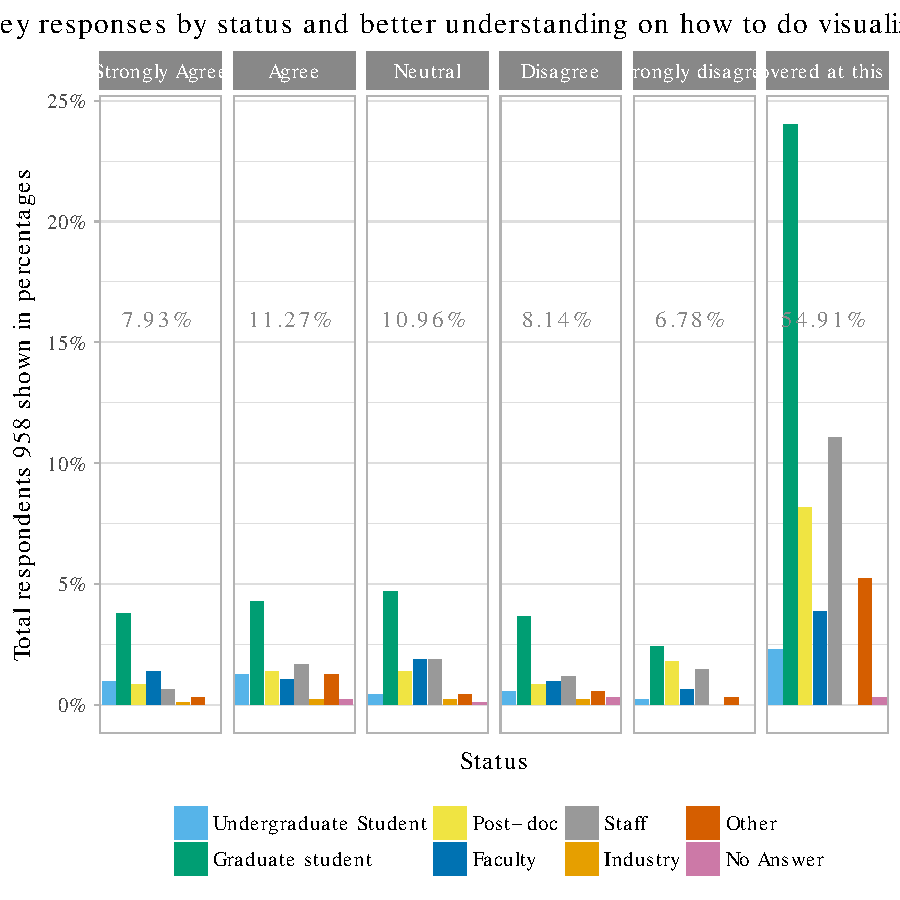
\includegraphics[width=.6\linewidth]{figure/calls-Rnwplotting-postsurvey-data-8} 

}


\begin{kframe}\begin{alltt}
\hlcom{# table(Epostworkshop$Import.R)}
\hlcom{# It seems like almost half (40%) of the workshops covered R}
\hlkwd{plotByStatusGeneric}\hlstd{(Epostworkshop,} \hlstr{"Post-survey"}\hlstd{,} \hlstr{"Import.R"} \hlstd{,} \hlstr{"better understanding on how to import a file in R and work with the data"}\hlstd{,}  \hlkwd{c}\hlstd{(}\hlnum{5}\hlstd{,}\hlnum{1}\hlstd{,}\hlnum{4}\hlstd{,}\hlnum{2}\hlstd{,}\hlnum{6}\hlstd{,}\hlnum{3}\hlstd{))}
\end{alltt}
\begin{verbatim}
## [1] 1081   44
## [1] "Import.R"
## [1] 967  44
## 
##                           Agree                        Disagree 
##                             281                              32 
## NA/Not covered at this workshop                         Neutral 
##                             159                              74 
##                  Strongly Agree               Strongly Disagree 
##                             391                              30 
## [1] "Strongly Agree"                  "Agree"                          
## [3] "Neutral"                         "Disagree"                       
## [5] "Strongly Disagree"               "NA/Not covered at this workshop"
\end{verbatim}
\end{kframe}

{\centering 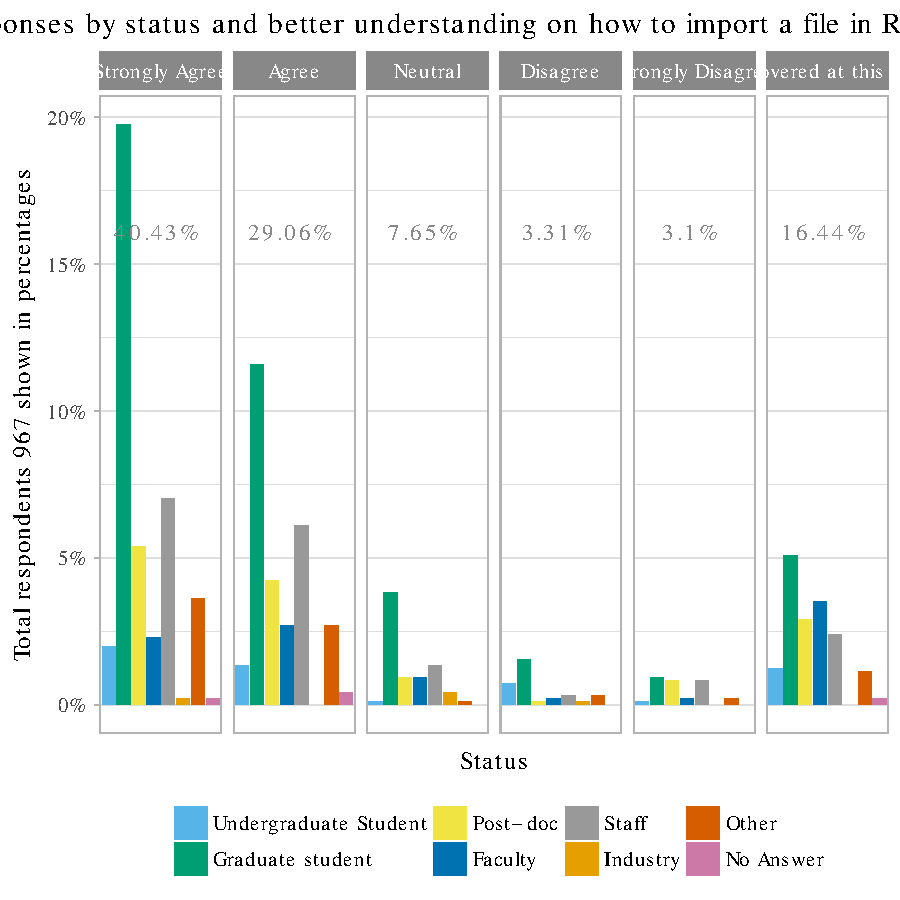
\includegraphics[width=.6\linewidth]{figure/calls-Rnwplotting-postsurvey-data-9} 

}


\begin{kframe}\begin{alltt}
\hlcom{# table(Epostworkshop$Visualizations.in.R)}
\hlkwd{plotByStatusGeneric}\hlstd{(Epostworkshop,} \hlstr{"Post-survey"}\hlstd{,} \hlstr{"Visualizations.in.R"} \hlstd{,} \hlstr{"better understanding on how to do visualizations in R"}\hlstd{,}  \hlkwd{c}\hlstd{(}\hlnum{5}\hlstd{,}\hlnum{1}\hlstd{,}\hlnum{4}\hlstd{,}\hlnum{2}\hlstd{,}\hlnum{6}\hlstd{,}\hlnum{3}\hlstd{))}
\end{alltt}
\begin{verbatim}
## [1] 1081   44
## [1] "Visualizations.in.R"
## [1] 960  44
## 
##                           Agree                        Disagree 
##                             307                              26 
## NA/Not covered at this workshop                         Neutral 
##                             163                              73 
##                  Strongly Agree               Strongly disagree 
##                             361                              30 
## [1] "Strongly Agree"                  "Agree"                          
## [3] "Neutral"                         "Disagree"                       
## [5] "Strongly disagree"               "NA/Not covered at this workshop"
\end{verbatim}
\end{kframe}

{\centering 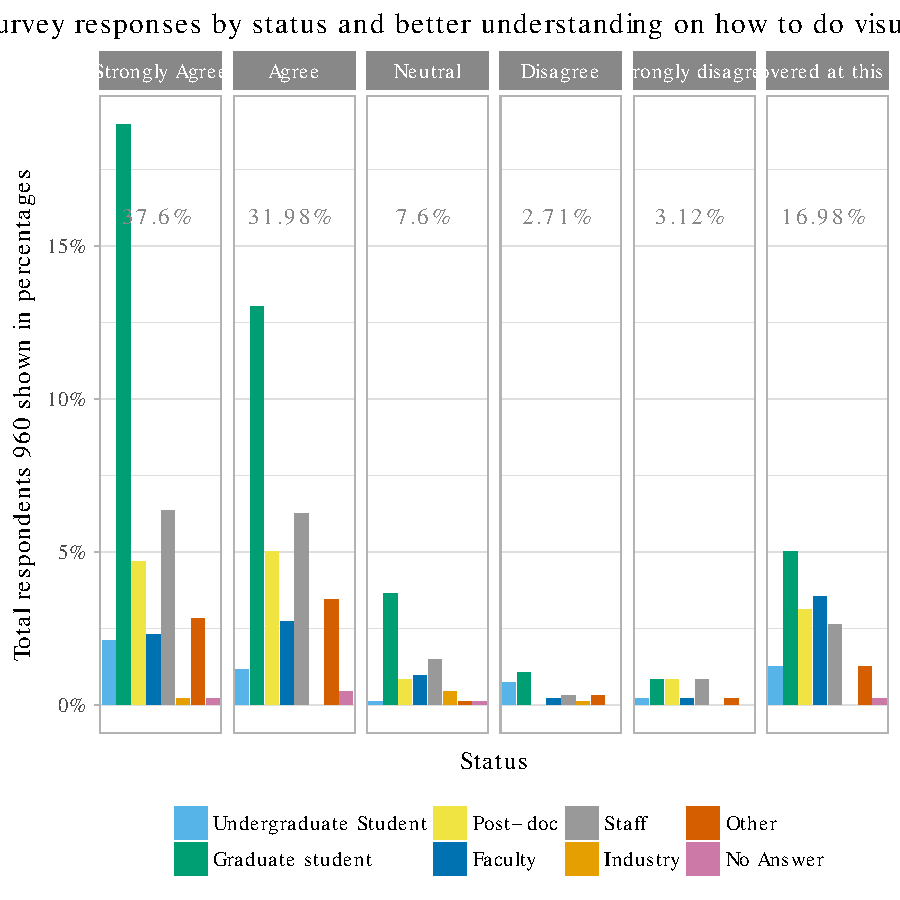
\includegraphics[width=.6\linewidth]{figure/calls-Rnwplotting-postsurvey-data-10} 

}


\begin{kframe}\begin{alltt}
\hlcom{# table(Epostworkshop$Construct.SQL)}
\hlkwd{plotByStatusGeneric}\hlstd{(Epostworkshop,} \hlstr{"Post-survey"}\hlstd{,} \hlstr{"Construct.SQL"} \hlstd{,} \hlstr{"better understanding on how to construct SQL queries"}\hlstd{,}  \hlkwd{c}\hlstd{(}\hlnum{5}\hlstd{,}\hlnum{1}\hlstd{,}\hlnum{4}\hlstd{,}\hlnum{2}\hlstd{,}\hlnum{6}\hlstd{,}\hlnum{3}\hlstd{))}
\end{alltt}
\begin{verbatim}
## [1] 1081   44
## [1] "Construct.SQL"
## [1] 948  44
## 
##                           Agree                        Disagree 
##                             208                              52 
## NA/Not covered at this workshop                         Neutral 
##                             334                             106 
##                  Strongly Agree               Strongly disagree 
##                             203                              45 
## [1] "Strongly Agree"                  "Agree"                          
## [3] "Neutral"                         "Disagree"                       
## [5] "Strongly disagree"               "NA/Not covered at this workshop"
\end{verbatim}
\end{kframe}

{\centering 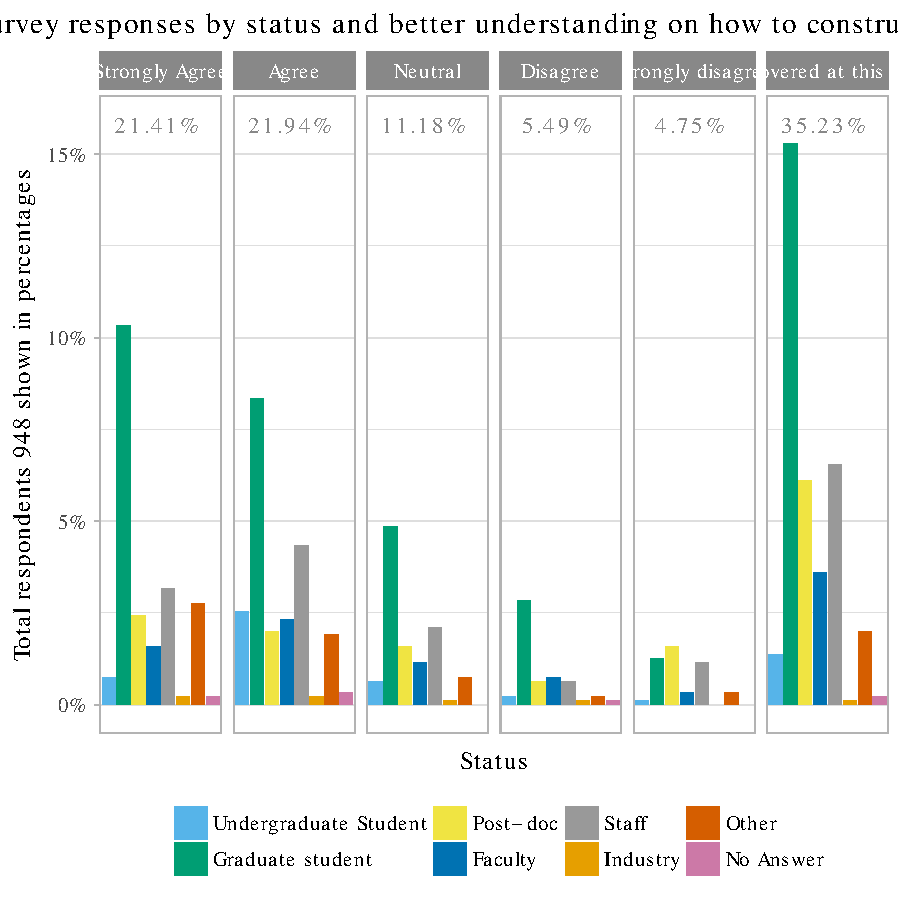
\includegraphics[width=.6\linewidth]{figure/calls-Rnwplotting-postsurvey-data-11} 

}


\begin{kframe}\begin{alltt}
\hlcom{# table(Epostworkshop$Use.command.line)}
\hlkwd{plotByStatusGeneric}\hlstd{(Epostworkshop,} \hlstr{"Post-survey"}\hlstd{,} \hlstr{"Use.command.line"} \hlstd{,} \hlstr{"better understanding on how to use command line"}\hlstd{,}  \hlkwd{c}\hlstd{(}\hlnum{5}\hlstd{,}\hlnum{1}\hlstd{,}\hlnum{4}\hlstd{,}\hlnum{2}\hlstd{,}\hlnum{6}\hlstd{,}\hlnum{3}\hlstd{))}
\end{alltt}
\begin{verbatim}
## [1] 1081   44
## [1] "Use.command.line"
## [1] 949  44
## 
##                           Agree                        Disagree 
##                             267                              32 
## NA/Not covered at this workshop                         Neutral 
##                             190                             120 
##                  Strongly Agree               Strongly disagree 
##                             313                              27 
## [1] "Strongly Agree"                  "Agree"                          
## [3] "Neutral"                         "Disagree"                       
## [5] "Strongly disagree"               "NA/Not covered at this workshop"
\end{verbatim}
\end{kframe}

{\centering 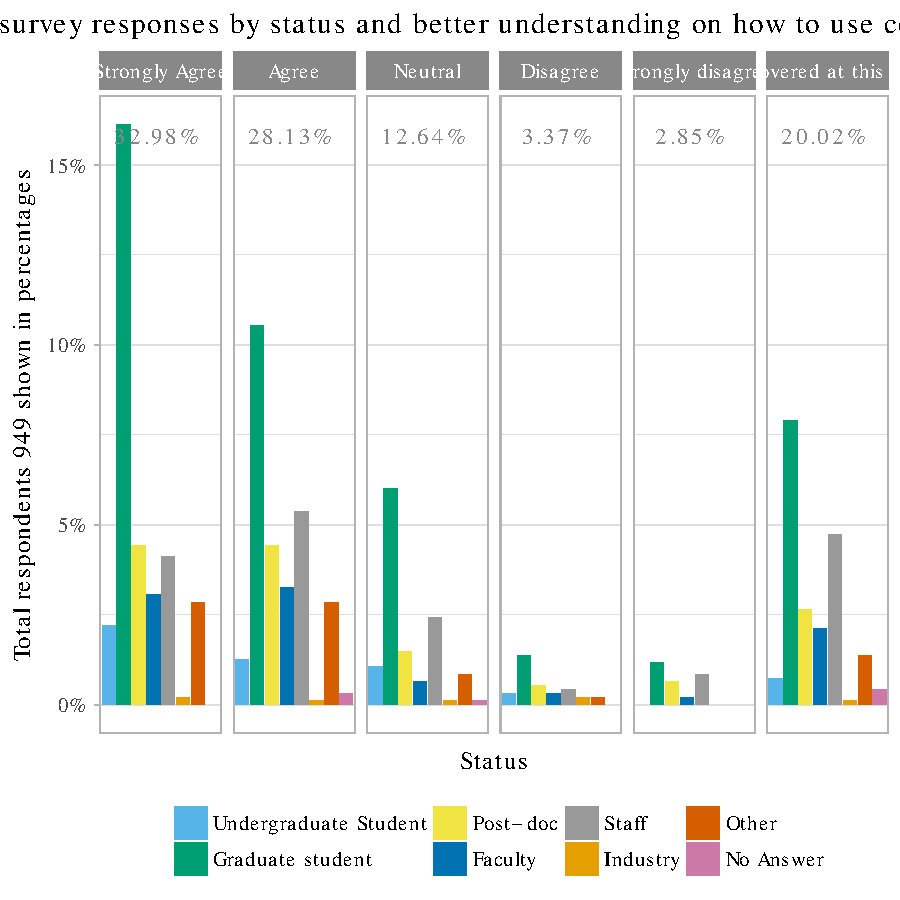
\includegraphics[width=.6\linewidth]{figure/calls-Rnwplotting-postsurvey-data-12} 

}


\begin{kframe}\begin{alltt}
\hlcom{# table(Epostworkshop$Skill.Level.Prior)}
\hlkwd{plotByStatusGeneric}\hlstd{(Epostworkshop,} \hlstr{"Post-survey"}\hlstd{,} \hlstr{"Skill.Level.Prior"} \hlstd{,} \hlstr{"data management and analysis skills prior the workshop"}\hlstd{,} \hlkwd{c}\hlstd{(}\hlnum{4}\hlstd{,}\hlnum{1}\hlstd{,}\hlnum{3}\hlstd{,}\hlnum{2}\hlstd{,}\hlnum{5}\hlstd{))}
\end{alltt}
\begin{verbatim}
## [1] 1081   44
## [1] "Skill.Level.Prior"
## [1] 969  44
## 
##                 High                  Low Neither high nor low            Very high 
##                  218                  230                  402                   14 
##             Very low 
##                  105 
## [1] "Very high"            "High"                 "Neither high nor low"
## [4] "Low"                  "Very low"
\end{verbatim}
\end{kframe}

{\centering 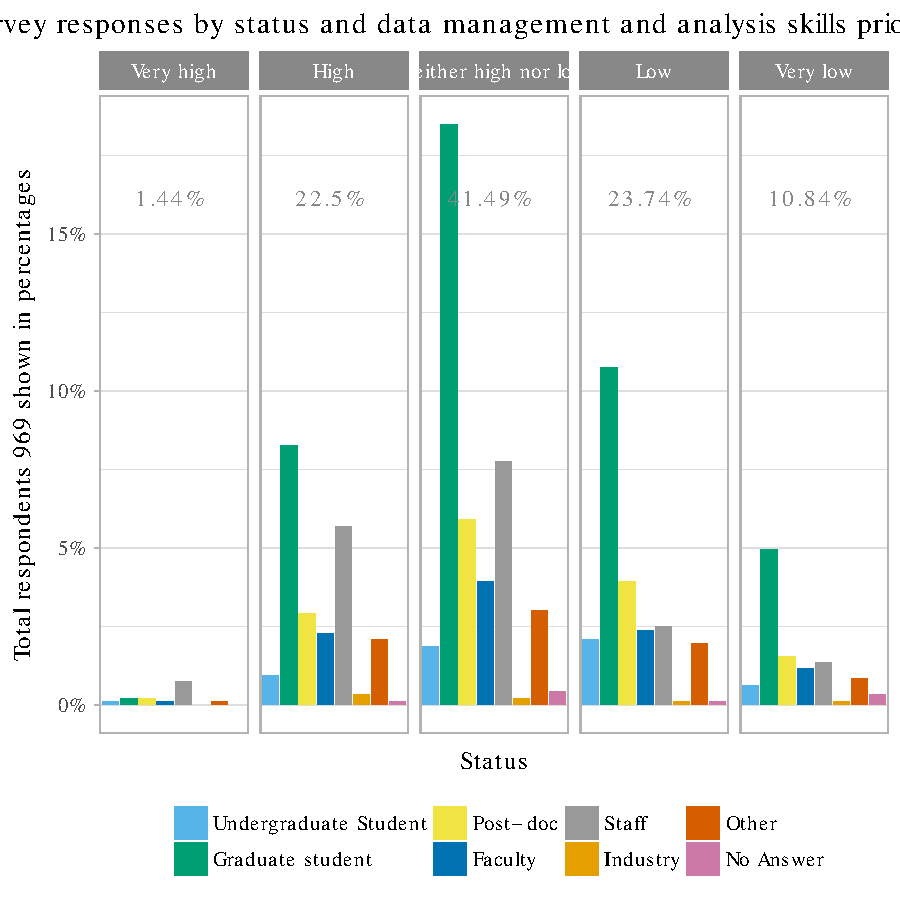
\includegraphics[width=.6\linewidth]{figure/calls-Rnwplotting-postsurvey-data-13} 

}


\begin{kframe}\begin{alltt}
\hlcom{# Combined plot}
\hlkwd{plotGeneric}\hlstd{(Epostworkshop,} \hlstr{"Post-survey"}\hlstd{,} \hlstr{"Skill.Level.Prior"} \hlstd{,}
            \hlstr{"skills prior the workshop vs level of involvement"}\hlstd{,} \hlkwd{c}\hlstd{(}\hlnum{4}\hlstd{,}\hlnum{1}\hlstd{,}\hlnum{3}\hlstd{,}\hlnum{2}\hlstd{,}\hlnum{5}\hlstd{),}\hlstr{"Involvement"}\hlstd{,} \hlkwd{c}\hlstd{(}\hlnum{3}\hlstd{,}\hlnum{1}\hlstd{,}\hlnum{2}\hlstd{))}
\end{alltt}
\begin{verbatim}
## [1] 1081   44
## [1] "Skill.Level.Prior"
## [1] "Involvement"
## [1] 964  44
## [1] "Very high"            "High"                 "Neither high nor low"
## [4] "Low"                  "Very low"            
## [1] "Very involved"             "Enthusiastically involved" "Somewhat involved"        
##                       
##                        Very involved Enthusiastically involved Somewhat involved
##   Very high                        3                         7                 4
##   High                           113                        78                24
##   Neither high nor low           188                       148                65
##   Low                            130                        71                29
##   Very low                        54                        33                17
\end{verbatim}
\end{kframe}

{\centering 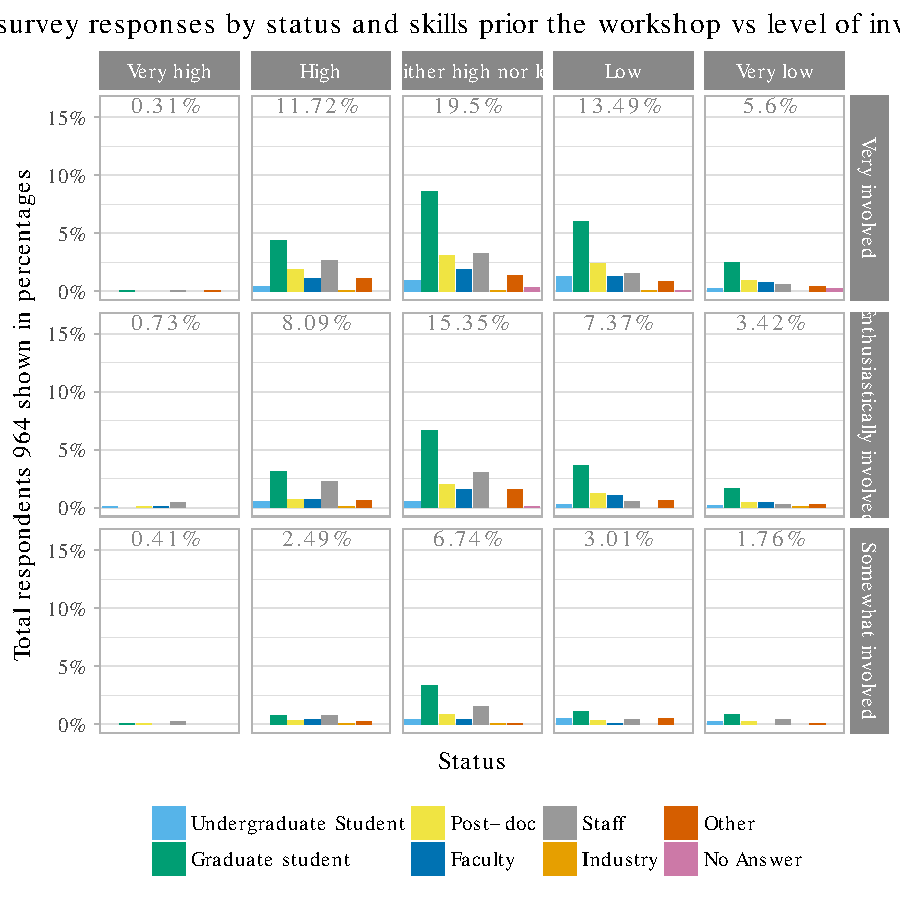
\includegraphics[width=.6\linewidth]{figure/calls-Rnwplotting-postsurvey-data-14} 

}


\begin{kframe}\begin{alltt}
\hlcom{# table(Epostworkshop$Skill.Level.Following)}
\hlkwd{plotByStatusGeneric}\hlstd{(Epostworkshop,} \hlstr{"Post-survey"}\hlstd{,} \hlstr{"Skill.Level.Following"} \hlstd{,} \hlstr{"data management and analysis skills following the workshop"}\hlstd{,} \hlkwd{c}\hlstd{(}\hlnum{3}\hlstd{,}\hlnum{2}\hlstd{,}\hlnum{4}\hlstd{,}\hlnum{1}\hlstd{))}
\end{alltt}
\begin{verbatim}
## [1] 1081   44
## [1] "Skill.Level.Following"
## [1] 972  44
## 
##  About the same          Higher     Much higher Somewhat higher 
##              75             355              63             479 
## [1] "Much higher"     "Higher"          "Somewhat higher" "About the same"
\end{verbatim}
\end{kframe}

{\centering 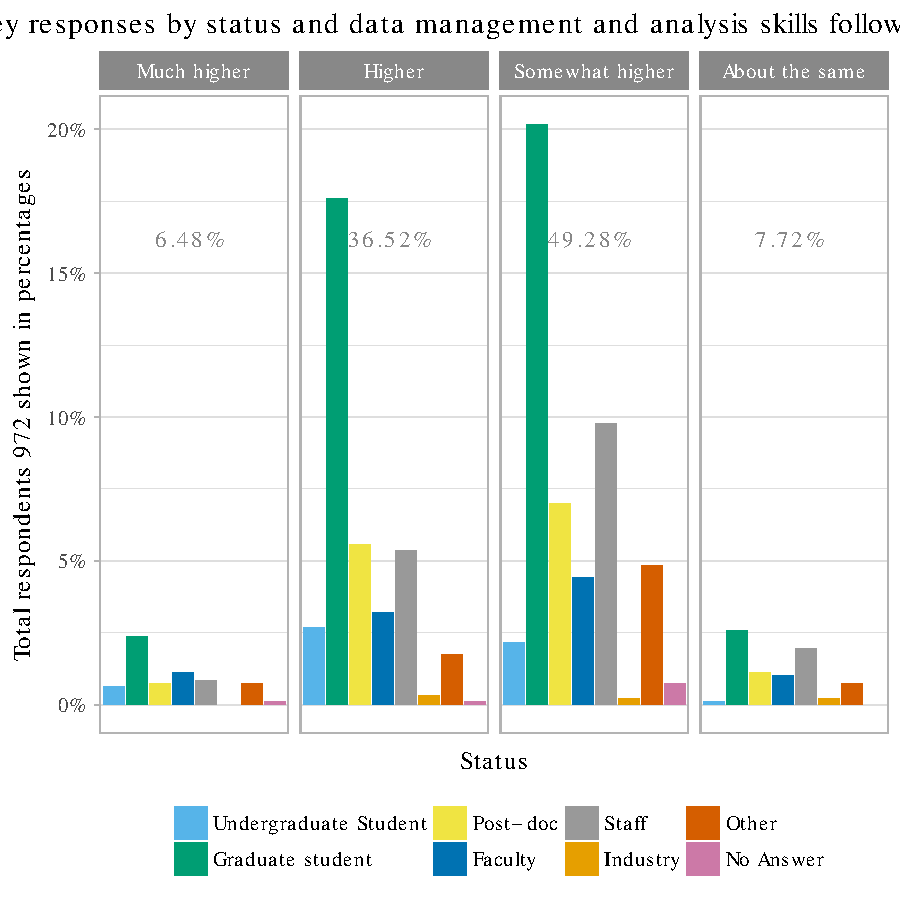
\includegraphics[width=.6\linewidth]{figure/calls-Rnwplotting-postsurvey-data-15} 

}


\begin{kframe}\begin{alltt}
\hlcom{# Combined plot}
\hlkwd{plotGeneric}\hlstd{(Epostworkshop,} \hlstr{"Post-survey"}\hlstd{,} \hlstr{"Skill.Level.Following"} \hlstd{,}
            \hlstr{"skills level following the workshop vs level of involvement"}\hlstd{,}  \hlkwd{c}\hlstd{(}\hlnum{3}\hlstd{,}\hlnum{2}\hlstd{,}\hlnum{4}\hlstd{,}\hlnum{1}\hlstd{),}\hlstr{"Involvement"}\hlstd{,} \hlkwd{c}\hlstd{(}\hlnum{3}\hlstd{,}\hlnum{1}\hlstd{,}\hlnum{2}\hlstd{))}
\end{alltt}
\begin{verbatim}
## [1] 1081   44
## [1] "Skill.Level.Following"
## [1] "Involvement"
## [1] 967  44
## [1] "Much higher"     "Higher"          "Somewhat higher" "About the same" 
## [1] "Very involved"             "Enthusiastically involved" "Somewhat involved"        
##                  
##                   Very involved Enthusiastically involved Somewhat involved
##   Much higher                18                        39                 4
##   Higher                    169                       158                27
##   Somewhat higher           266                       121                90
##   About the same             38                        19                18
\end{verbatim}
\end{kframe}

{\centering 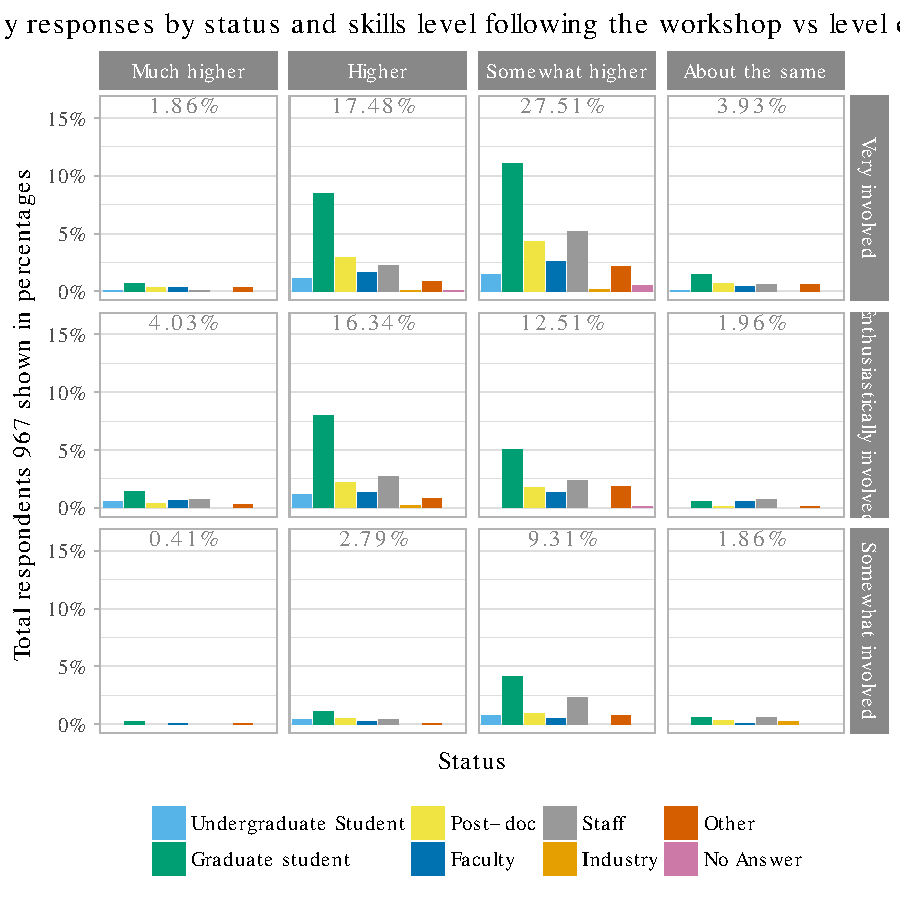
\includegraphics[width=.6\linewidth]{figure/calls-Rnwplotting-postsurvey-data-16} 

}


\begin{kframe}\begin{alltt}
\hlcom{# table(Epostworkshop$Application)}
\hlkwd{plotByStatusGeneric}\hlstd{(Epostworkshop,} \hlstr{"Post-survey"}\hlstd{,} \hlstr{"Application"} \hlstd{,} \hlstr{"can immediately applied what was learned at the workshop"}\hlstd{,} \hlkwd{c}\hlstd{(}\hlnum{4}\hlstd{,}\hlnum{1}\hlstd{,}\hlnum{3}\hlstd{,}\hlnum{2}\hlstd{,}\hlnum{5}\hlstd{))}
\end{alltt}
\begin{verbatim}
## [1] 1081   44
## [1] "Application"
## [1] 965  44
## 
##             Agree          Disagree           Neutral    Strongly agree Strongly disagree 
##               496                55               168               232                14 
## [1] "Strongly agree"    "Agree"             "Neutral"           "Disagree"         
## [5] "Strongly disagree"
\end{verbatim}
\end{kframe}

{\centering 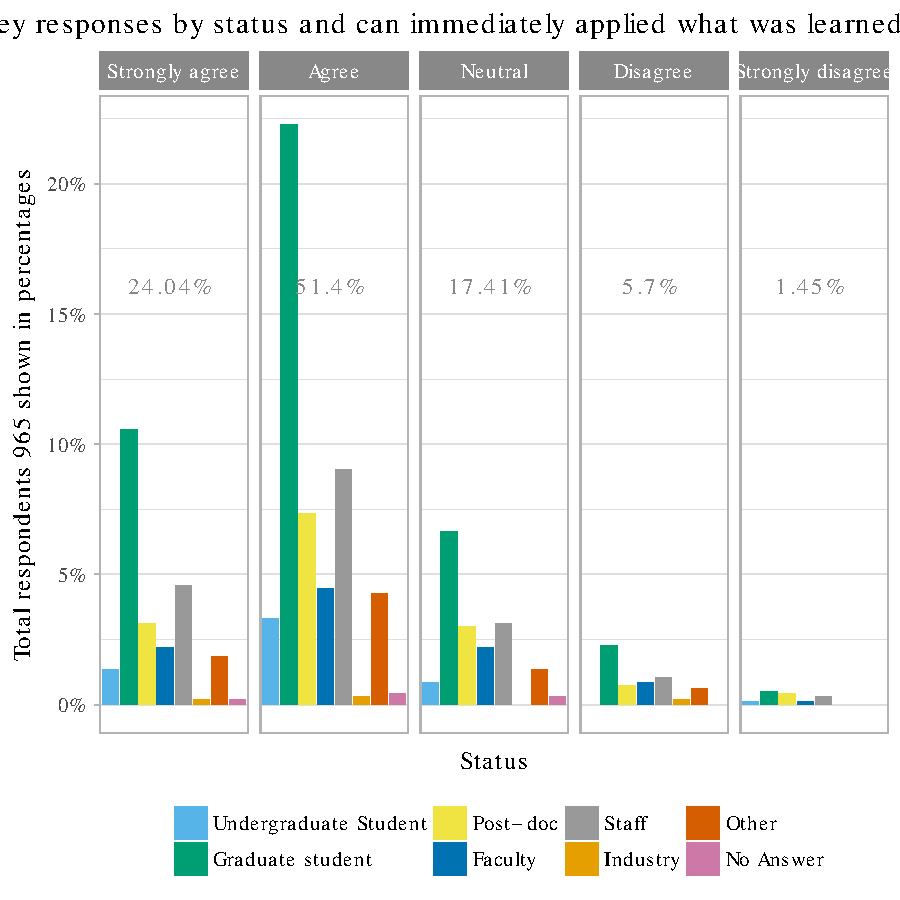
\includegraphics[width=.6\linewidth]{figure/calls-Rnwplotting-postsurvey-data-17} 

}


\begin{kframe}\begin{alltt}
\hlcom{# Combined plot}
\hlkwd{plotGeneric}\hlstd{(Epostworkshop,} \hlstr{"Post-survey"}\hlstd{,} \hlstr{"Application"} \hlstd{,}
            \hlstr{"can immediately applied what was learned vs level of involvement"}\hlstd{,}  \hlkwd{c}\hlstd{(}\hlnum{4}\hlstd{,}\hlnum{1}\hlstd{,}\hlnum{3}\hlstd{,}\hlnum{2}\hlstd{,}\hlnum{5}\hlstd{),}\hlstr{"Involvement"}\hlstd{,} \hlkwd{c}\hlstd{(}\hlnum{3}\hlstd{,}\hlnum{1}\hlstd{,}\hlnum{2}\hlstd{))}
\end{alltt}
\begin{verbatim}
## [1] 1081   44
## [1] "Application"
## [1] "Involvement"
## [1] 961  44
## [1] "Strongly agree"    "Agree"             "Neutral"           "Disagree"         
## [5] "Strongly disagree"
## [1] "Very involved"             "Enthusiastically involved" "Somewhat involved"        
##                    
##                     Very involved Enthusiastically involved Somewhat involved
##   Strongly agree               83                       136                12
##   Agree                       269                       152                74
##   Neutral                      98                        27                42
##   Disagree                     31                        15                 9
##   Strongly disagree             5                         6                 2
\end{verbatim}
\end{kframe}

{\centering 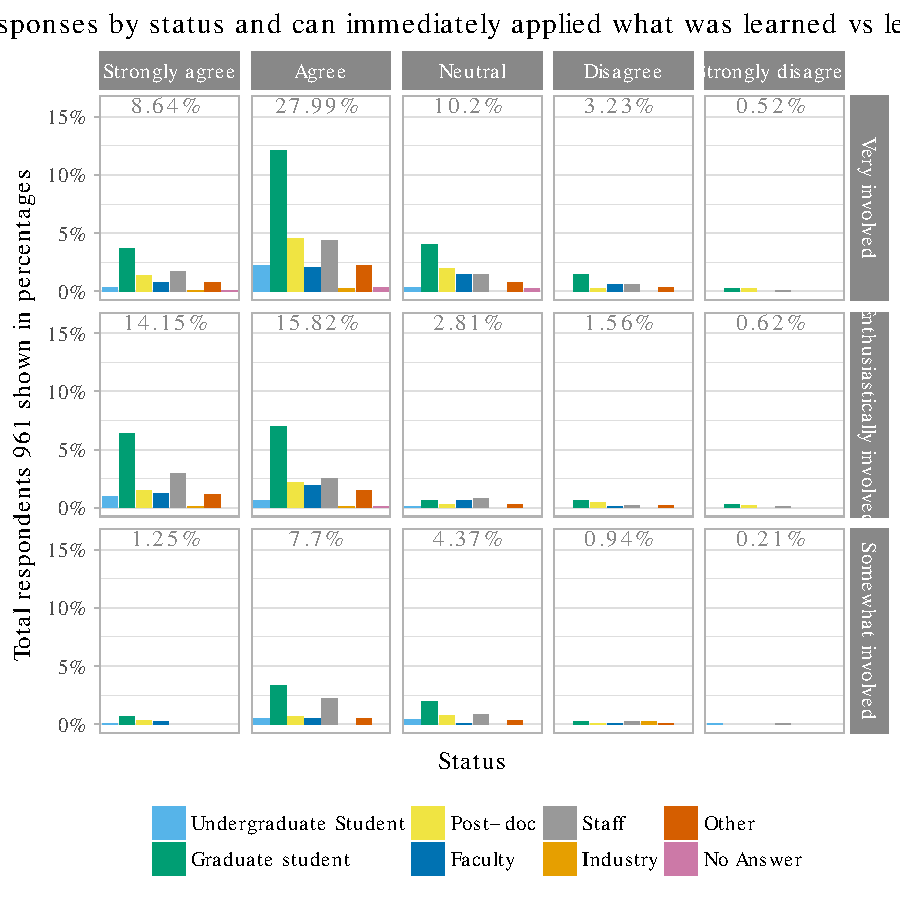
\includegraphics[width=.6\linewidth]{figure/calls-Rnwplotting-postsurvey-data-18} 

}


\begin{kframe}\begin{alltt}
\hlcom{# needs to be a big squared plot}
\hlkwd{plotGeneric}\hlstd{(Epostworkshop,} \hlstr{"Post-survey"}\hlstd{,} \hlstr{"Application"} \hlstd{,}
            \hlstr{"can immediately applied what was learned vs skill level prior the workshop"}\hlstd{,}  \hlkwd{c}\hlstd{(}\hlnum{4}\hlstd{,}\hlnum{1}\hlstd{,}\hlnum{3}\hlstd{,}\hlnum{2}\hlstd{,}\hlnum{5}\hlstd{),}\hlstr{"Skill.Level.Prior"}\hlstd{,} \hlkwd{c}\hlstd{(}\hlnum{4}\hlstd{,}\hlnum{1}\hlstd{,}\hlnum{3}\hlstd{,}\hlnum{2}\hlstd{,}\hlnum{5}\hlstd{))}
\end{alltt}
\begin{verbatim}
## [1] 1081   44
## [1] "Application"
## [1] "Skill.Level.Prior"
## [1] 960  44
## [1] "Strongly agree"    "Agree"             "Neutral"           "Disagree"         
## [5] "Strongly disagree"
## [1] "Very high"            "High"                 "Neither high nor low"
## [4] "Low"                  "Very low"            
##                    
##                     Very high High Neither high nor low Low Very low
##   Strongly agree            5   68                  106  42        9
##   Agree                     9  109                  195 134       46
##   Neutral                   0   22                   66  40       40
##   Disagree                  0   10                   29  10        6
##   Strongly disagree         0    3                    4   4        3
\end{verbatim}
\end{kframe}

{\centering 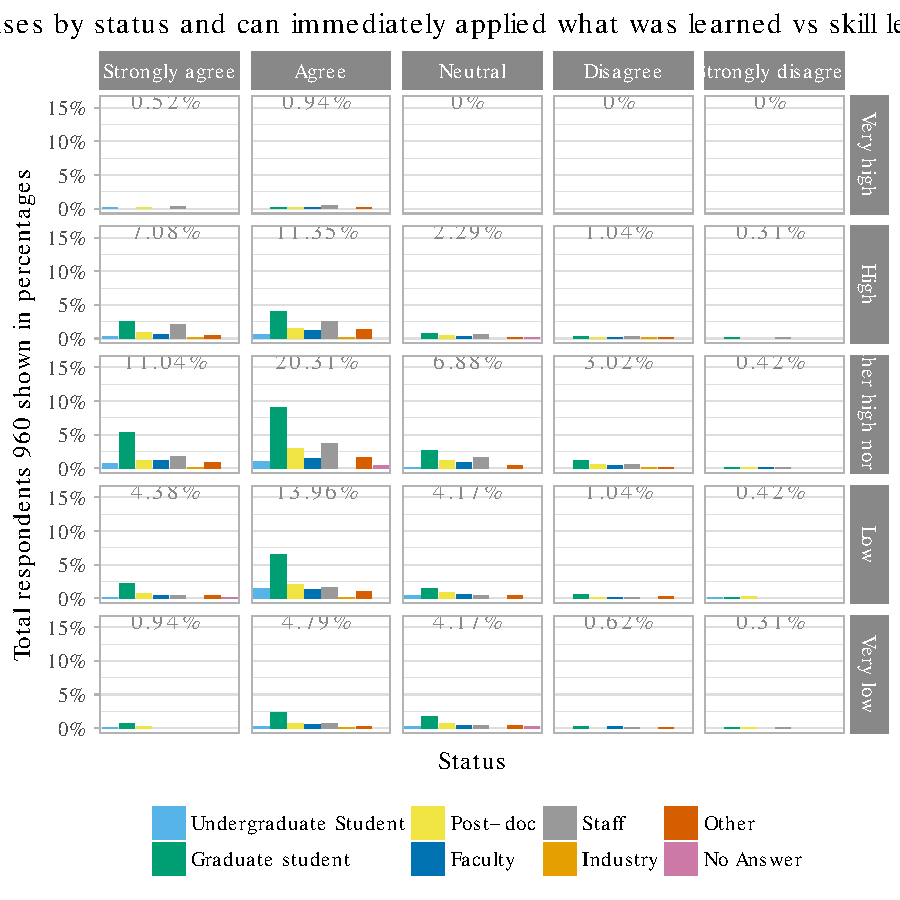
\includegraphics[width=.6\linewidth]{figure/calls-Rnwplotting-postsurvey-data-19} 

}


\begin{kframe}\begin{alltt}
\hlcom{# table(Epostworkshop$Worth.My.Time)}
\hlkwd{plotByStatusGeneric}\hlstd{(Epostworkshop,} \hlstr{"Post-survey"}\hlstd{,} \hlstr{"Worth.My.Time"} \hlstd{,} \hlstr{"the workshop was worth my time"}\hlstd{,} \hlkwd{c}\hlstd{(}\hlnum{4}\hlstd{,}\hlnum{1}\hlstd{,}\hlnum{3}\hlstd{,}\hlnum{2}\hlstd{,}\hlnum{5}\hlstd{))}
\end{alltt}
\begin{verbatim}
## [1] 1081   44
## [1] "Worth.My.Time"
## [1] 967  44
## 
##             Agree          Disagree           Neutral    Strongly agree Strongly disagree 
##               408                23                49               470                17 
## [1] "Strongly agree"    "Agree"             "Neutral"           "Disagree"         
## [5] "Strongly disagree"
\end{verbatim}
\end{kframe}

{\centering 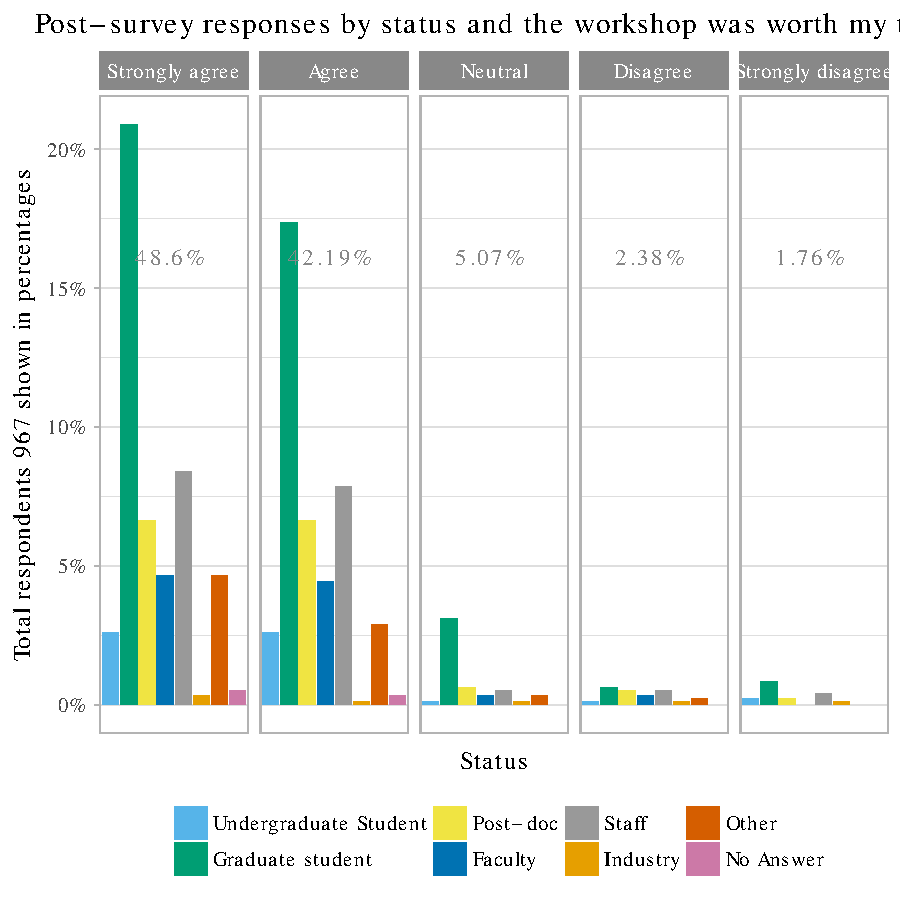
\includegraphics[width=.6\linewidth]{figure/calls-Rnwplotting-postsurvey-data-20} 

}


\begin{kframe}\begin{alltt}
\hlcom{# Combined plot}
\hlkwd{plotGeneric}\hlstd{(Epostworkshop,} \hlstr{"Post-survey"}\hlstd{,} \hlstr{"Worth.My.Time"} \hlstd{,}
            \hlstr{"the workshop was worth my time vs level of involvement"}\hlstd{,}  \hlkwd{c}\hlstd{(}\hlnum{4}\hlstd{,}\hlnum{1}\hlstd{,}\hlnum{3}\hlstd{,}\hlnum{2}\hlstd{,}\hlnum{5}\hlstd{),}\hlstr{"Involvement"}\hlstd{,} \hlkwd{c}\hlstd{(}\hlnum{3}\hlstd{,}\hlnum{1}\hlstd{,}\hlnum{2}\hlstd{))}
\end{alltt}
\begin{verbatim}
## [1] 1081   44
## [1] "Worth.My.Time"
## [1] "Involvement"
## [1] 964  44
## [1] "Strongly agree"    "Agree"             "Neutral"           "Disagree"         
## [5] "Strongly disagree"
## [1] "Very involved"             "Enthusiastically involved" "Somewhat involved"        
##                    
##                     Very involved Enthusiastically involved Somewhat involved
##   Strongly agree              205                       232                32
##   Agree                       235                        92                80
##   Neutral                      30                         4                15
##   Disagree                     12                         2                 8
##   Strongly disagree             6                         7                 4
\end{verbatim}
\end{kframe}

{\centering 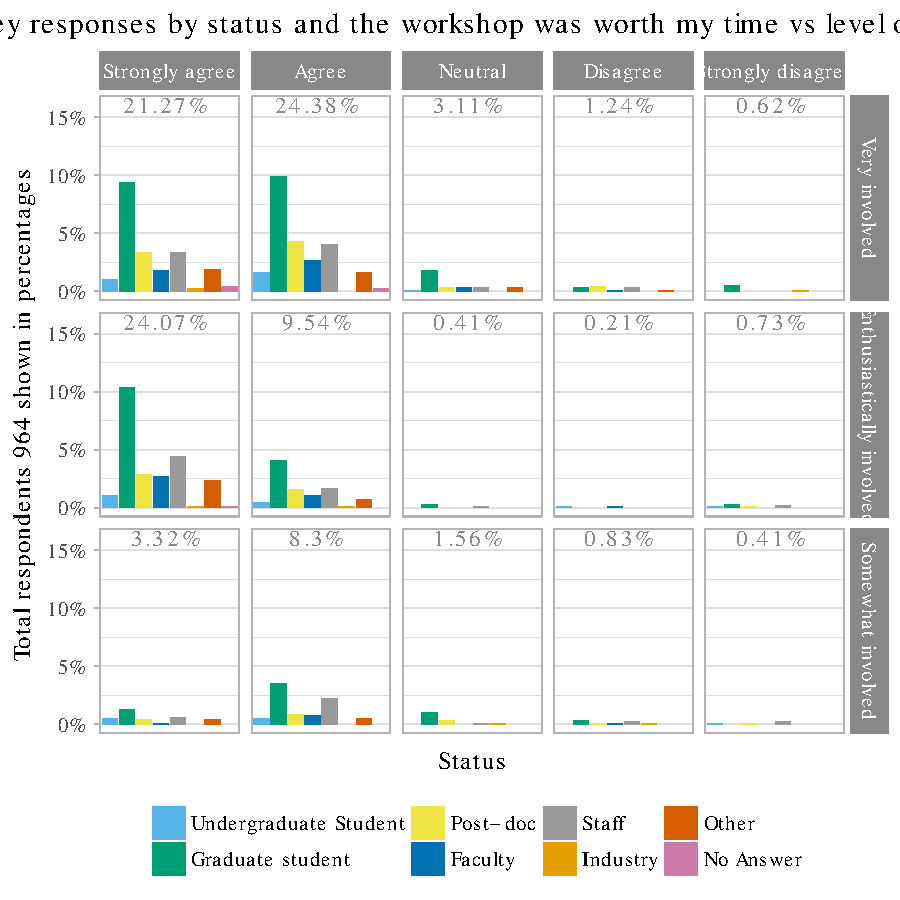
\includegraphics[width=.6\linewidth]{figure/calls-Rnwplotting-postsurvey-data-21} 

}


\begin{kframe}\begin{alltt}
\hlcom{# table(Epostworkshop$Material)}
\hlkwd{plotByStatusGeneric}\hlstd{(Epostworkshop,} \hlstr{"Post-survey"}\hlstd{,} \hlstr{"Material"} \hlstd{,} \hlstr{"the material matched the workshop description"}\hlstd{,} \hlkwd{c}\hlstd{(}\hlnum{4}\hlstd{,}\hlnum{1}\hlstd{,}\hlnum{3}\hlstd{,}\hlnum{2}\hlstd{,}\hlnum{5}\hlstd{))}
\end{alltt}
\begin{verbatim}
## [1] 1081   44
## [1] "Material"
## [1] 966  44
## 
##             Agree          Disagree           Neutral    Strongly agree Strongly disagree 
##               465                28                60               395                18 
## [1] "Strongly agree"    "Agree"             "Neutral"           "Disagree"         
## [5] "Strongly disagree"
\end{verbatim}
\end{kframe}

{\centering 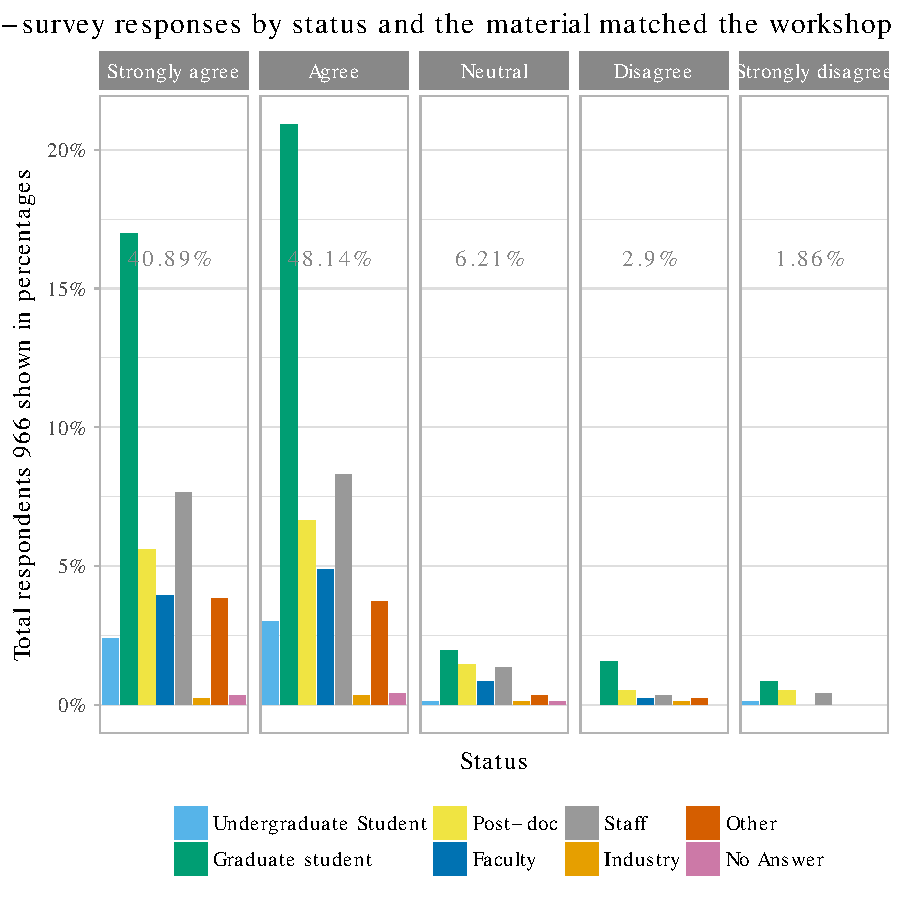
\includegraphics[width=.6\linewidth]{figure/calls-Rnwplotting-postsurvey-data-22} 

}


\begin{kframe}\begin{alltt}
\hlcom{# table(Epostworkshop$Recommend)}
\hlkwd{plotByStatusGeneric}\hlstd{(Epostworkshop,} \hlstr{"Post-survey"}\hlstd{,} \hlstr{"Recommend"} \hlstd{,} \hlstr{"would recommend the workshop"}\hlstd{,} \hlkwd{c}\hlstd{(}\hlnum{4}\hlstd{,}\hlnum{1}\hlstd{,}\hlnum{3}\hlstd{,}\hlnum{2}\hlstd{,}\hlnum{5}\hlstd{))}
\end{alltt}
\begin{verbatim}
## [1] 1081   44
## [1] "Recommend"
## [1] 593  44
## 
##             Agree          Disagree           Neutral    Strongly agree Strongly disagree 
##               261                 7                31               285                 9 
## [1] "Strongly agree"    "Agree"             "Neutral"           "Disagree"         
## [5] "Strongly disagree"
\end{verbatim}
\end{kframe}

{\centering 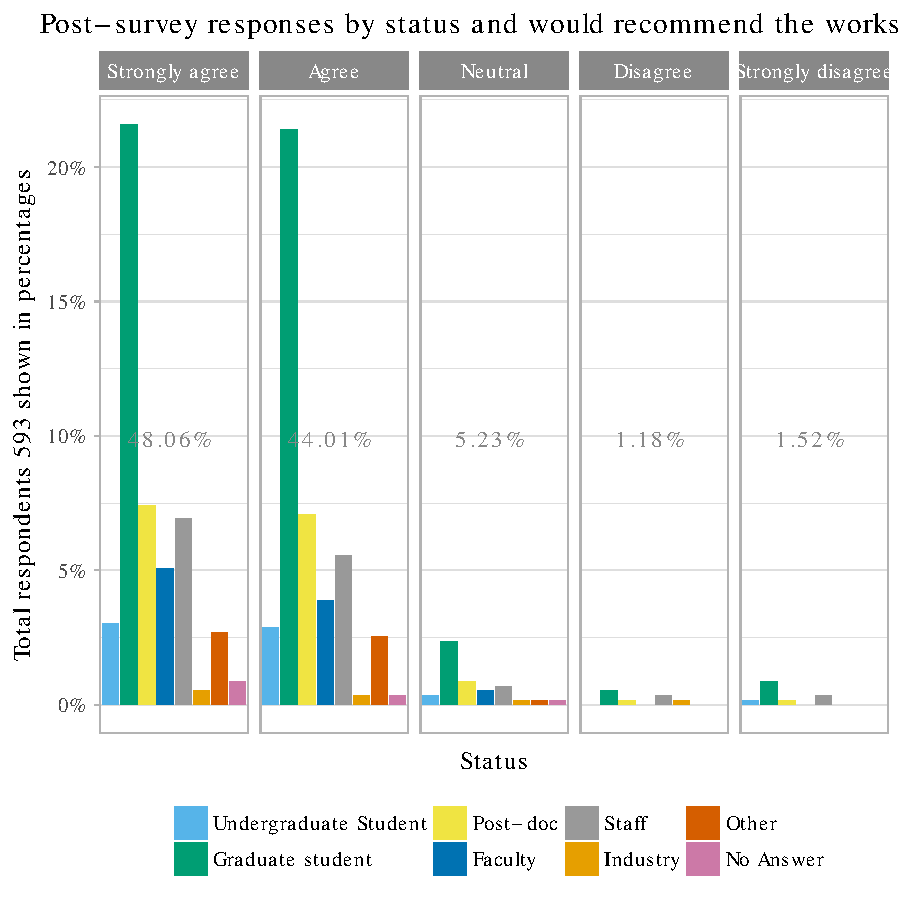
\includegraphics[width=.6\linewidth]{figure/calls-Rnwplotting-postsurvey-data-23} 

}


\begin{kframe}\begin{alltt}
\hlcom{# Combined plot # big square plot}
\hlcom{# great relationship}
\hlkwd{plotGeneric}\hlstd{(Epostworkshop,} \hlstr{"Post-survey"}\hlstd{,} \hlstr{"Worth.My.Time"} \hlstd{,}
            \hlstr{"the workshop was worth my time vs I will recommend this workshop"}\hlstd{,}  \hlkwd{c}\hlstd{(}\hlnum{4}\hlstd{,}\hlnum{1}\hlstd{,}\hlnum{3}\hlstd{,}\hlnum{2}\hlstd{,}\hlnum{5}\hlstd{),}\hlstr{"Recommend"}\hlstd{,} \hlkwd{c}\hlstd{(}\hlnum{4}\hlstd{,}\hlnum{1}\hlstd{,}\hlnum{3}\hlstd{,}\hlnum{2}\hlstd{,}\hlnum{5}\hlstd{))}
\end{alltt}
\begin{verbatim}
## [1] 1081   44
## [1] "Worth.My.Time"
## [1] "Recommend"
## [1] 592  44
## [1] "Strongly agree"    "Agree"             "Neutral"           "Disagree"         
## [5] "Strongly disagree"
## [1] "Strongly agree"    "Agree"             "Neutral"           "Disagree"         
## [5] "Strongly disagree"
##                    
##                     Strongly agree Agree Neutral Disagree Strongly disagree
##   Strongly agree               227    45       0        0                 0
##   Agree                         52   198      15        0                 0
##   Neutral                        4    12      12        1                 0
##   Disagree                       1     5       3        5                 1
##   Strongly disagree              1     0       1        1                 8
\end{verbatim}
\end{kframe}

{\centering 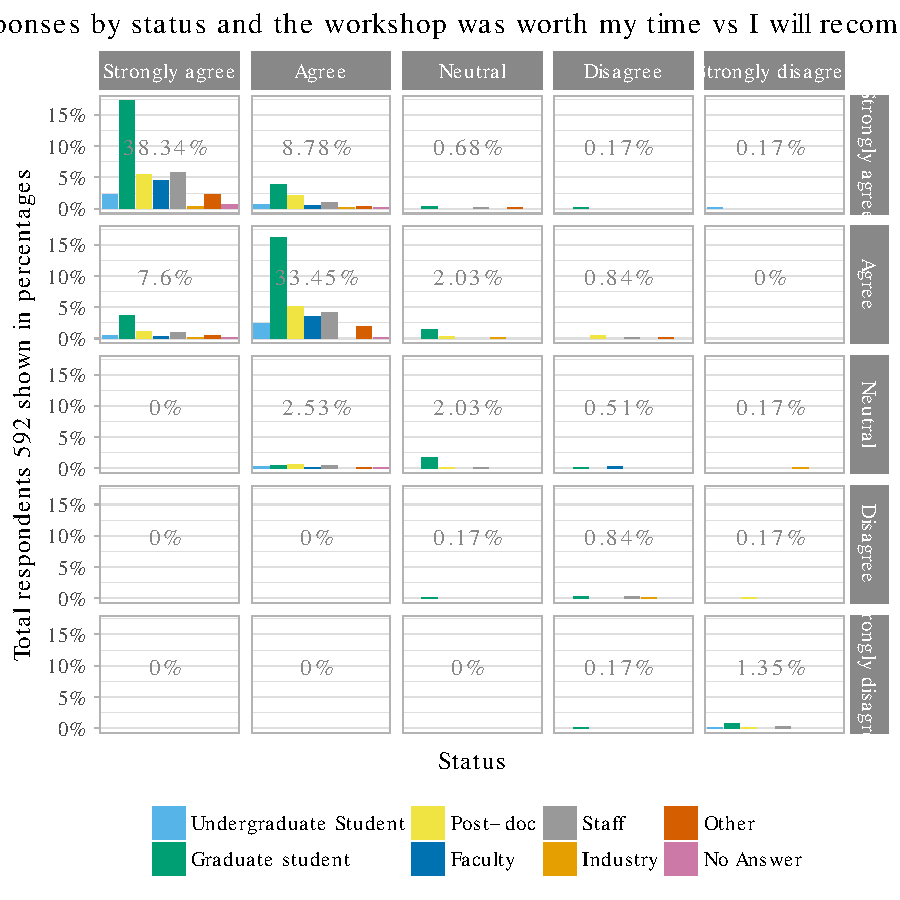
\includegraphics[width=.6\linewidth]{figure/calls-Rnwplotting-postsurvey-data-24} 

}


\begin{kframe}\begin{alltt}
\hlcom{# Combined plot}
\hlkwd{plotGeneric}\hlstd{(Epostworkshop,} \hlstr{"Post-survey"}\hlstd{,} \hlstr{"Recommend"} \hlstd{,}
            \hlstr{"I will recommend this workshop vs level of involvement"}\hlstd{,}  \hlkwd{c}\hlstd{(}\hlnum{4}\hlstd{,}\hlnum{1}\hlstd{,}\hlnum{3}\hlstd{,}\hlnum{2}\hlstd{,}\hlnum{5}\hlstd{),}\hlstr{"Involvement"}\hlstd{,} \hlkwd{c}\hlstd{(}\hlnum{3}\hlstd{,}\hlnum{1}\hlstd{,}\hlnum{2}\hlstd{))}
\end{alltt}
\begin{verbatim}
## [1] 1081   44
## [1] "Recommend"
## [1] "Involvement"
## [1] 590  44
## [1] "Strongly agree"    "Agree"             "Neutral"           "Disagree"         
## [5] "Strongly disagree"
## [1] "Very involved"             "Enthusiastically involved" "Somewhat involved"        
##                    
##                     Very involved Enthusiastically involved Somewhat involved
##   Strongly agree              111                       140                33
##   Agree                       157                        65                38
##   Neutral                      19                         3                 8
##   Disagree                      4                         0                 3
##   Strongly disagree             3                         4                 2
\end{verbatim}
\end{kframe}

{\centering 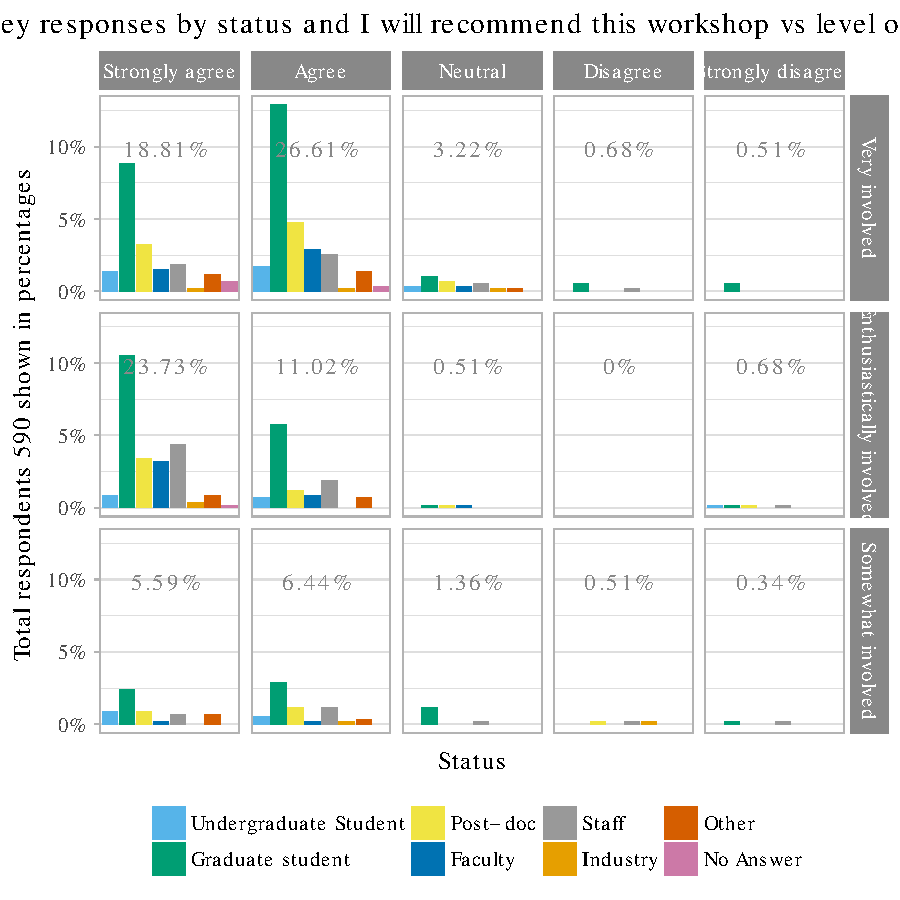
\includegraphics[width=.6\linewidth]{figure/calls-Rnwplotting-postsurvey-data-25} 

}


\begin{kframe}\begin{alltt}
\hlcom{# Combined plot}
\hlkwd{plotGeneric}\hlstd{(Epostworkshop,} \hlstr{"Post-survey"}\hlstd{,} \hlstr{"Recommend"} \hlstd{,}
            \hlstr{"I will recommend this workshop vs it was worth my time"}\hlstd{,}  \hlkwd{c}\hlstd{(}\hlnum{4}\hlstd{,}\hlnum{1}\hlstd{,}\hlnum{3}\hlstd{,}\hlnum{2}\hlstd{,}\hlnum{5}\hlstd{),}\hlstr{"Worth.My.Time"}\hlstd{,} \hlkwd{c}\hlstd{(}\hlnum{4}\hlstd{,}\hlnum{1}\hlstd{,}\hlnum{3}\hlstd{,}\hlnum{2}\hlstd{,}\hlnum{5}\hlstd{))}
\end{alltt}
\begin{verbatim}
## [1] 1081   44
## [1] "Recommend"
## [1] "Worth.My.Time"
## [1] 592  44
## [1] "Strongly agree"    "Agree"             "Neutral"           "Disagree"         
## [5] "Strongly disagree"
## [1] "Strongly agree"    "Agree"             "Neutral"           "Disagree"         
## [5] "Strongly disagree"
##                    
##                     Strongly agree Agree Neutral Disagree Strongly disagree
##   Strongly agree               227    52       4        1                 1
##   Agree                         45   198      12        5                 0
##   Neutral                        0    15      12        3                 1
##   Disagree                       0     0       1        5                 1
##   Strongly disagree              0     0       0        1                 8
\end{verbatim}
\end{kframe}

{\centering 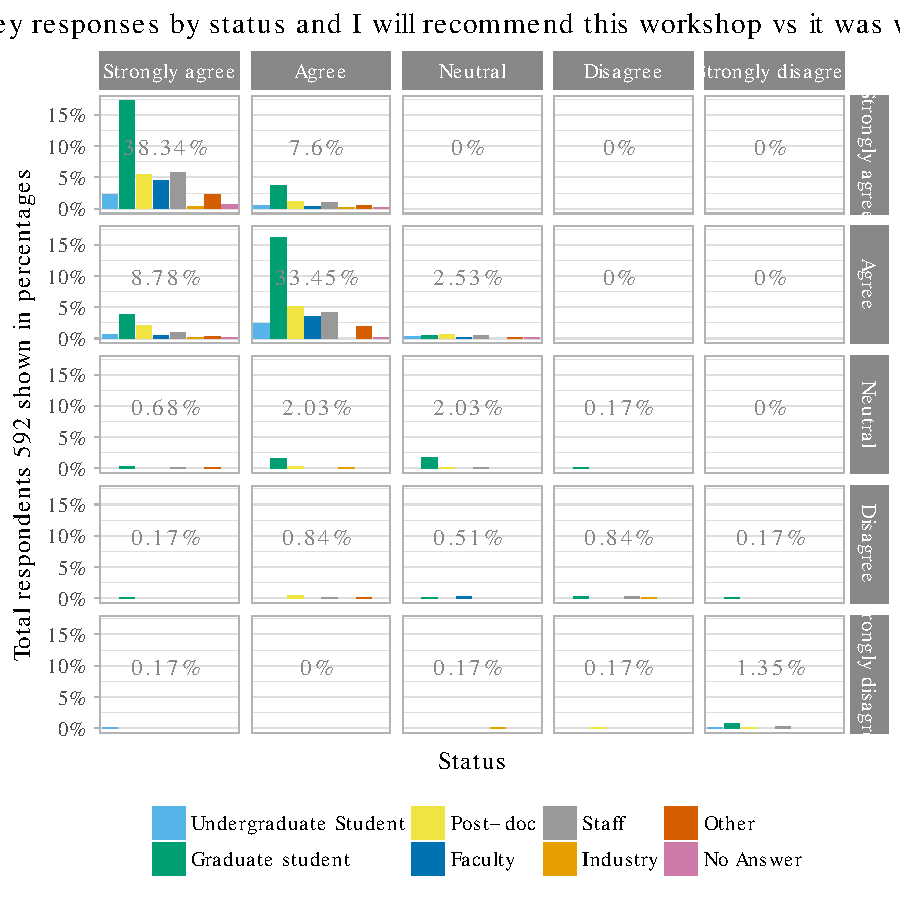
\includegraphics[width=.6\linewidth]{figure/calls-Rnwplotting-postsurvey-data-26} 

}


\begin{kframe}\begin{alltt}
\hlcom{# table(Epostworkshop$Instructors.Effective)}
\hlkwd{plotByStatusGeneric}\hlstd{(Epostworkshop,} \hlstr{"Post-survey"}\hlstd{,} \hlstr{"Instructors.Effective"} \hlstd{,} \hlstr{"were the instructors effective in teaching the workshop?"}\hlstd{,} \hlkwd{c}\hlstd{(}\hlnum{1}\hlstd{,}\hlnum{2}\hlstd{,}\hlnum{5}\hlstd{,}\hlnum{4}\hlstd{,}\hlnum{3}\hlstd{))}
\end{alltt}
\begin{verbatim}
## [1] 1081   44
## [1] "Instructors.Effective"
## [1] 955  44
## 
##           Always Most of the time            Never        Sometimes          Usually 
##              556              294                2               31               72 
## [1] "Always"           "Most of the time" "Usually"          "Sometimes"       
## [5] "Never"
\end{verbatim}
\end{kframe}

{\centering 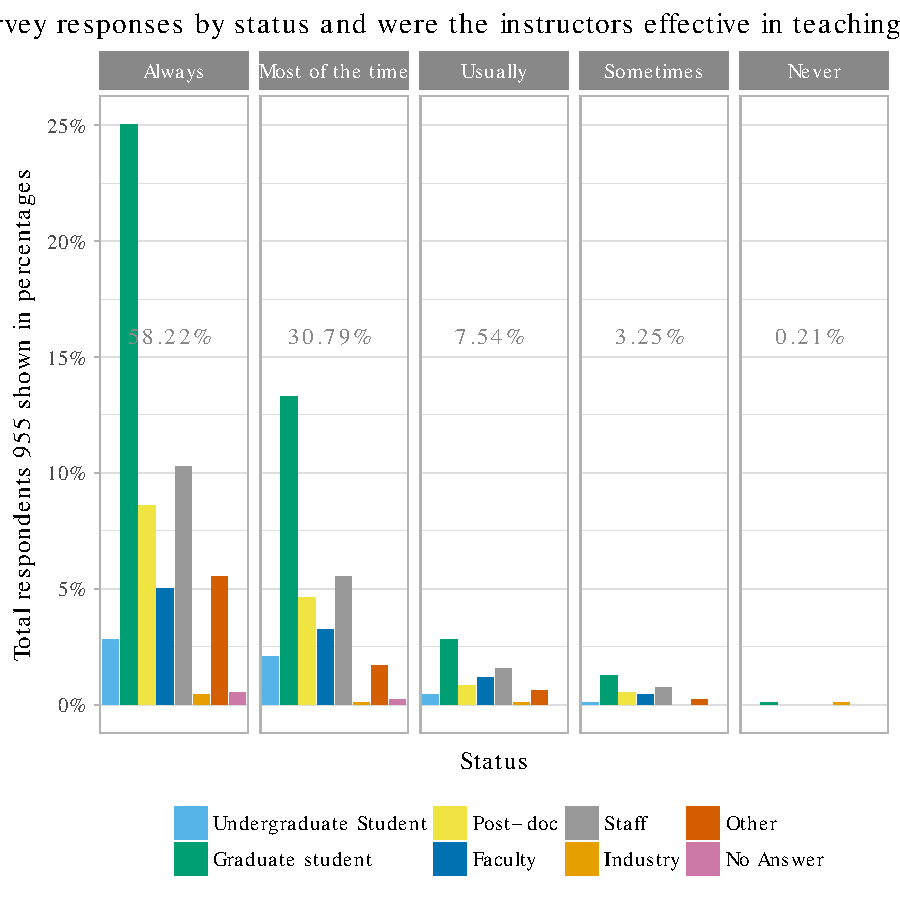
\includegraphics[width=.6\linewidth]{figure/calls-Rnwplotting-postsurvey-data-27} 

}


\begin{kframe}\begin{alltt}
\hlcom{# Combined plot}
\hlcom{# great relationship}
\hlkwd{plotGeneric}\hlstd{(Epostworkshop,} \hlstr{"Post-survey"}\hlstd{,} \hlstr{"Instructors.Effective"} \hlstd{,}
            \hlstr{"were the instructors effective in teaching vs I will recommend this workshop"}\hlstd{,}  \hlkwd{c}\hlstd{(}\hlnum{1}\hlstd{,}\hlnum{2}\hlstd{,}\hlnum{5}\hlstd{,}\hlnum{4}\hlstd{,}\hlnum{3}\hlstd{),}\hlstr{"Recommend"}\hlstd{,} \hlkwd{c}\hlstd{(}\hlnum{4}\hlstd{,}\hlnum{1}\hlstd{,}\hlnum{3}\hlstd{,}\hlnum{2}\hlstd{,}\hlnum{5}\hlstd{))}
\end{alltt}
\begin{verbatim}
## [1] 1081   44
## [1] "Instructors.Effective"
## [1] "Recommend"
## [1] 583  44
## [1] "Always"           "Most of the time" "Usually"          "Sometimes"       
## [5] "Never"           
## [1] "Strongly agree"    "Agree"             "Neutral"           "Disagree"         
## [5] "Strongly disagree"
##                   
##                    Strongly agree Agree Neutral Disagree Strongly disagree
##   Always                      202   123       7        2                 7
##   Most of the time             71    98      12        2                 1
##   Usually                       8    26       3        1                 0
##   Sometimes                     1     7       7        2                 1
##   Never                         0     1       1        0                 0
\end{verbatim}
\end{kframe}

{\centering 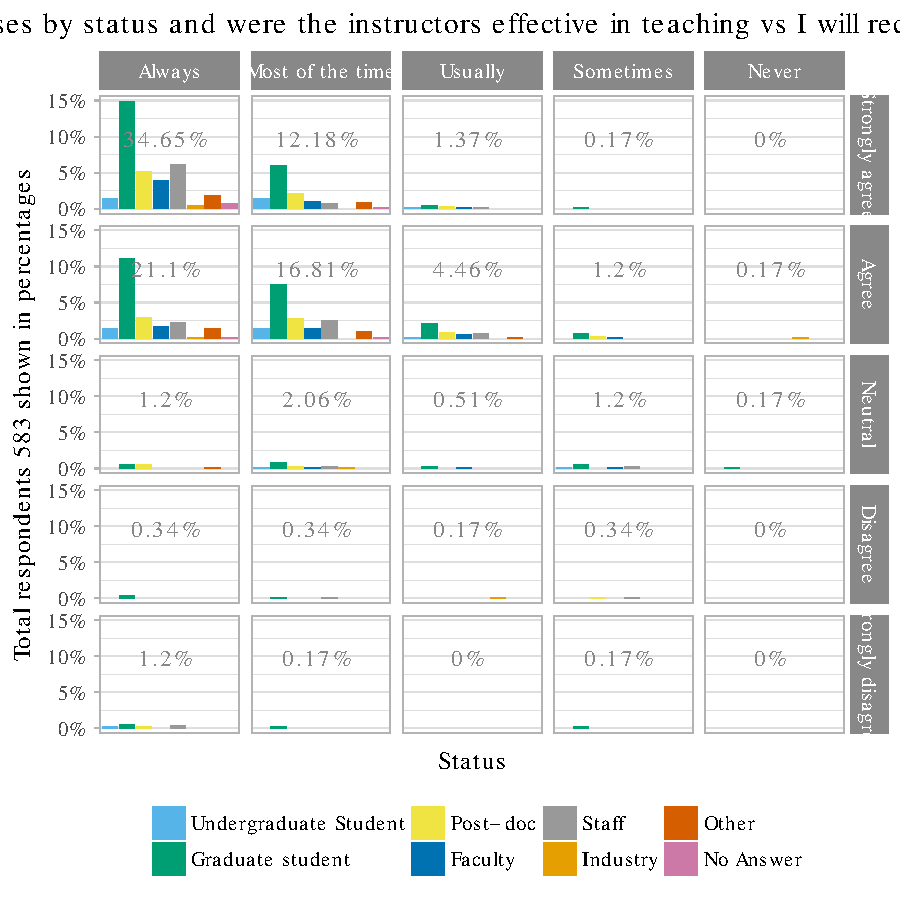
\includegraphics[width=.6\linewidth]{figure/calls-Rnwplotting-postsurvey-data-28} 

}


\begin{kframe}\begin{alltt}
\hlcom{# table(Epostworkshop$Instructors.Enthusiastic)}
\hlkwd{plotByStatusGeneric}\hlstd{(Epostworkshop,} \hlstr{"Post-survey"}\hlstd{,} \hlstr{"Instructors.Enthusiastic"} \hlstd{,} \hlstr{"were the instructors enthusiastic about the workshop?"}\hlstd{,} \hlkwd{c}\hlstd{(}\hlnum{1}\hlstd{,}\hlnum{2}\hlstd{,}\hlnum{4}\hlstd{,}\hlnum{3}\hlstd{))}
\end{alltt}
\begin{verbatim}
## [1] 1081   44
## [1] "Instructors.Enthusiastic"
## [1] 951  44
## 
##           Always Most of the time        Sometimes          Usually 
##              755              147                6               43 
## [1] "Always"           "Most of the time" "Usually"          "Sometimes"
\end{verbatim}
\end{kframe}

{\centering 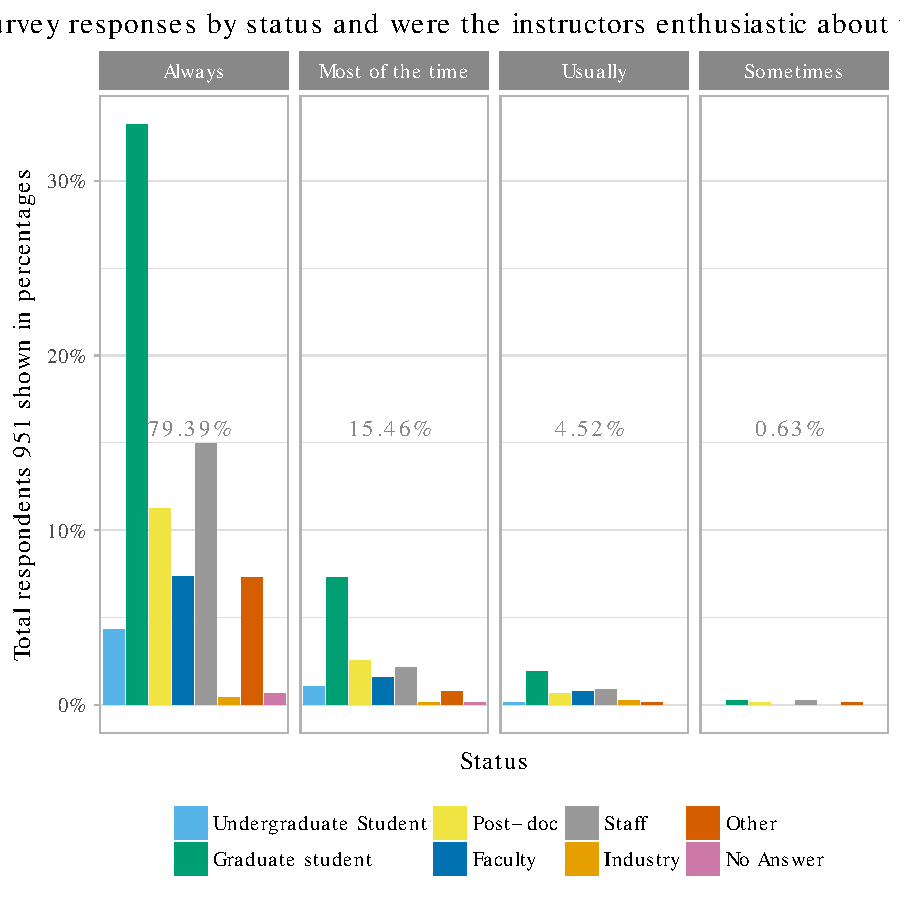
\includegraphics[width=.6\linewidth]{figure/calls-Rnwplotting-postsurvey-data-29} 

}


\begin{kframe}\begin{alltt}
\hlcom{# Combined plot}
\hlcom{# great relationship}
\hlkwd{plotGeneric}\hlstd{(Epostworkshop,} \hlstr{"Post-survey"}\hlstd{,} \hlstr{"Instructors.Effective"} \hlstd{,}
            \hlstr{"instructors were effective in teaching vs instructors were enthusiastic"}\hlstd{,}  \hlkwd{c}\hlstd{(}\hlnum{1}\hlstd{,}\hlnum{2}\hlstd{,}\hlnum{5}\hlstd{,}\hlnum{4}\hlstd{,}\hlnum{3}\hlstd{),}\hlstr{"Instructors.Enthusiastic"}\hlstd{,} \hlkwd{c}\hlstd{(}\hlnum{1}\hlstd{,}\hlnum{2}\hlstd{,}\hlnum{4}\hlstd{,}\hlnum{3}\hlstd{))}
\end{alltt}
\begin{verbatim}
## [1] 1081   44
## [1] "Instructors.Effective"
## [1] "Instructors.Enthusiastic"
## [1] 949  44
## [1] "Always"           "Most of the time" "Usually"          "Sometimes"       
## [5] "Never"           
## [1] "Always"           "Most of the time" "Usually"          "Sometimes"       
##                   
##                    Always Most of the time Usually Sometimes
##   Always              532               19       2         0
##   Most of the time    194               94       3         0
##   Usually              24               27      21         0
##   Sometimes             3                7      16         5
##   Never                 0                0       1         1
\end{verbatim}
\end{kframe}

{\centering 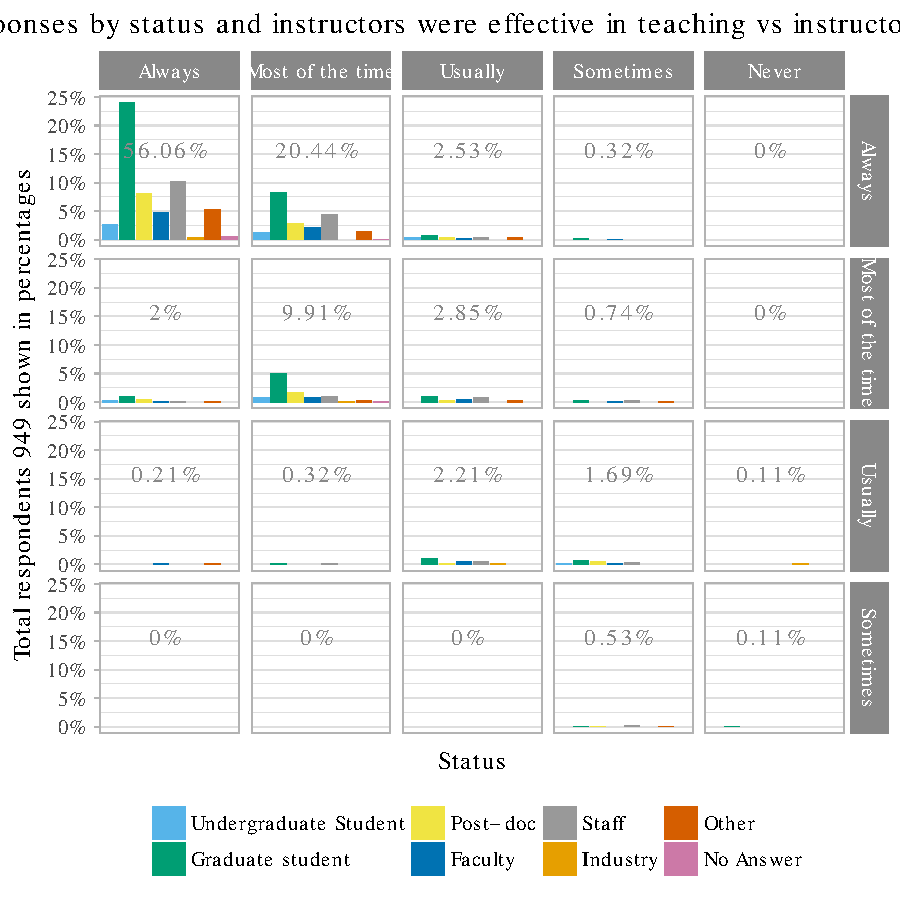
\includegraphics[width=.6\linewidth]{figure/calls-Rnwplotting-postsurvey-data-30} 

}



\end{knitrout}
\begin{knitrout}
\definecolor{shadecolor}{rgb}{0.969, 0.969, 0.969}\color{fgcolor}\begin{kframe}
\begin{alltt}
\hlcom{# table(Epostworkshop$Workshop.in.US) }
\hlkwd{plotByStatusGeneric}\hlstd{(Epostworkshop,} \hlstr{"Post-survey"}\hlstd{,} \hlstr{"Workshop.in.US"} \hlstd{,} \hlstr{"the workshop was in the US"}\hlstd{,} \hlkwd{c}\hlstd{(}\hlnum{2}\hlstd{,}\hlnum{1}\hlstd{))}
\end{alltt}
\begin{verbatim}
## [1] 1081   44
## [1] "Workshop.in.US"
## [1] 970  44
## 
##  No Yes 
## 283 687 
## [1] "Yes" "No"
\end{verbatim}
\end{kframe}

{\centering 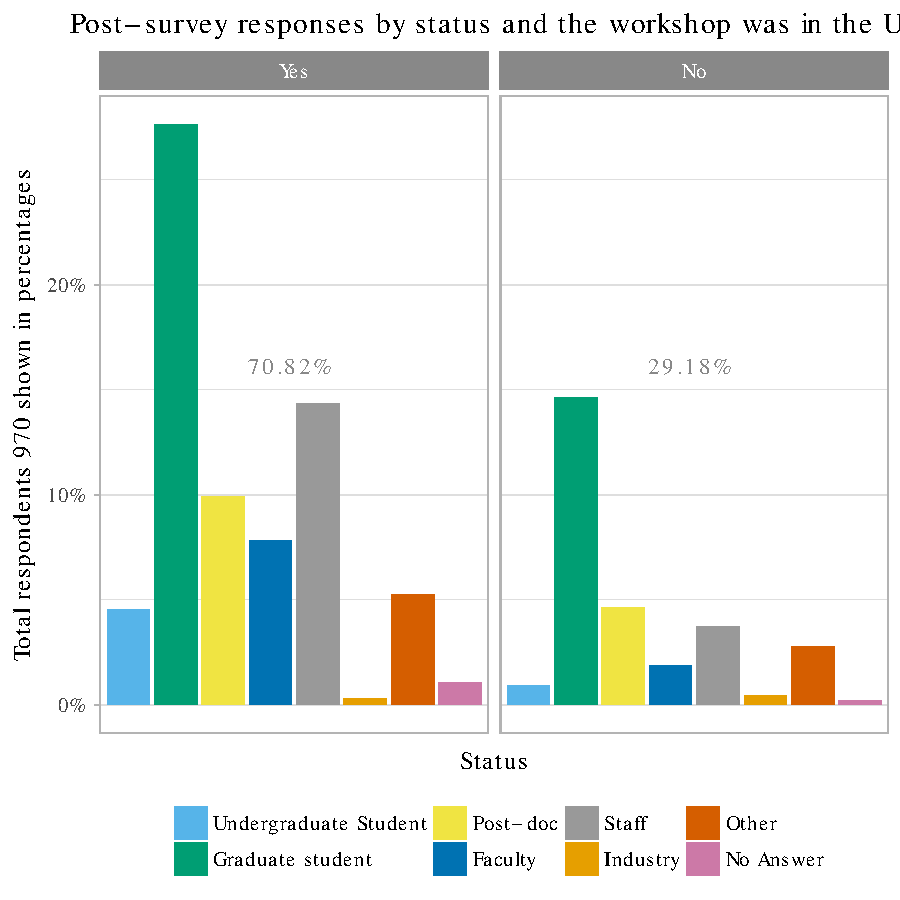
\includegraphics[width=.6\linewidth]{figure/calls-Rnwplotting-postsurvey-dataUS-1} 

}


\begin{kframe}\begin{alltt}
\hlcom{# # age and gender are not shown in the PDF questionnaire}
\hlcom{# # not very necesary as given in the presurvey}
\hlcom{# table(Epostworkshop$Age)}
\hlkwd{plotByStatusGeneric}\hlstd{(Epostworkshop,} \hlstr{"Post-survey"}\hlstd{,} \hlstr{"Age"} \hlstd{,} \hlstr{"age"}\hlstd{)}
\end{alltt}
\begin{verbatim}
## [1] 1081   44
## [1] "Age"
## [1] 387  44
## 
##             18-24             25-34             35-44             45-54             55-64 
##                66               205                65                30                12 
##             65-74 Prefer not to say 
##                 4                 5
\end{verbatim}
\end{kframe}

{\centering \includegraphics[width=.6\linewidth]{figure/calls-Rnwplotting-postsurvey-dataUS-2} 

}


\begin{kframe}\begin{alltt}
\hlcom{# table(Epostworkshop$Race.White) # given that is the majority}
\hlkwd{plotByStatusGeneric}\hlstd{(Epostworkshop,} \hlstr{"Post-survey"}\hlstd{,} \hlstr{"Race.White"} \hlstd{,} \hlstr{"white"}\hlstd{)}
\end{alltt}
\begin{verbatim}
## [1] 1081   44
## [1] "Race.White"
## [1] 405  44
## 
## White/Caucasian 
##             405
\end{verbatim}
\end{kframe}

{\centering \includegraphics[width=.6\linewidth]{figure/calls-Rnwplotting-postsurvey-dataUS-3} 

}


\begin{kframe}\begin{alltt}
\hlcom{# Filter all of those who did not take the survey in the US }
\hlstd{EpostworkshopUS} \hlkwb{<-} \hlkwd{subset}\hlstd{(Epostworkshop, Workshop.in.US} \hlopt{==} \hlstr{"Yes"}\hlstd{)}
\hlstd{EpostworkshopUS} \hlkwb{<-} \hlkwd{droplevels}\hlstd{(EpostworkshopUS)}
\hlcom{# table(EpostworkshopUS$Workshop.in.US)}
\hlcom{# table(EpostworkshopUS$Gender)}
\hlkwd{plotByStatusGeneric}\hlstd{(EpostworkshopUS,} \hlstr{"Post-survey"}\hlstd{,} \hlstr{"Gender"} \hlstd{,} \hlstr{"gender"}\hlstd{)}
\end{alltt}
\begin{verbatim}
## [1] 687  44
## [1] "Gender"
## [1] 687  44
## 
##            Female              Male Prefer not to say         No Answer 
##               200               129                15               343
\end{verbatim}
\end{kframe}

{\centering \includegraphics[width=.6\linewidth]{figure/calls-Rnwplotting-postsurvey-dataUS-4} 

}


\begin{kframe}\begin{alltt}
\hlcom{# ############################################################################}
\end{alltt}
\end{kframe}
\end{knitrout}
\begin{knitrout}
\definecolor{shadecolor}{rgb}{0.969, 0.969, 0.969}\color{fgcolor}\begin{kframe}
\begin{alltt}
\hlcom{# not very interesting}
\hlkwd{multiplot}\hlstd{(}\hlkwd{plotByGender}\hlstd{(EpreworkshopUS,} \hlstr{"Pre- survey"}\hlstd{),}
          \hlkwd{plotByGender}\hlstd{(EpostworkshopUS,} \hlstr{"Post- survey"}\hlstd{),} \hlkwc{cols}\hlstd{=}\hlnum{2}\hlstd{)}
\end{alltt}
\end{kframe}

{\centering \includegraphics[width=.6\linewidth]{figure/calls-Rnwplotting-pre-postsurvey-dataUS-1} 

}


\begin{kframe}\begin{alltt}
\hlcom{# Gender and status only US surveys}
\hlkwd{plotByGenderStatus}\hlstd{(EpreworkshopUS,} \hlstr{"Pre-survey"}\hlstd{)}
\end{alltt}
\end{kframe}

{\centering \includegraphics[width=.6\linewidth]{figure/calls-Rnwplotting-pre-postsurvey-dataUS-2} 

}


\begin{kframe}\begin{alltt}
\hlkwd{plotByGenderStatus}\hlstd{(EpostworkshopUS,} \hlstr{"Post-survey"}\hlstd{)}
\end{alltt}
\end{kframe}

{\centering \includegraphics[width=.6\linewidth]{figure/calls-Rnwplotting-pre-postsurvey-dataUS-3} 

}


\begin{kframe}\begin{alltt}
\hlcom{# filter not answered}
\hlstd{newpreGS} \hlkwb{<-} \hlkwd{ExcludeNANotGiven}\hlstd{(Epreworkshop)}
\end{alltt}
\begin{verbatim}
##      Gender    Status
## 1      Male  Post-doc
## 2      Male     Staff
## 3 No Answer     Other
## 4    Female     Other
## 5 No Answer No Answer
## 6      Male     Staff
## 'data.frame':	2343 obs. of  2 variables:
##  $ Gender: Factor w/ 4 levels "Female","Male",..: 2 2 4 1 4 2 2 2 2 1 ...
##  $ Status: Factor w/ 8 levels "Undergraduate Student",..: 3 5 7 7 8 5 2 5 4 5 ...
## NULL
## 
##            Female              Male Prefer not to say         No Answer 
##               717               540                22              1064 
##                    Status
## Gender              Undergraduate Student Graduate Student Post-doc Faculty Staff
##   Female                               35              304       80      64   160
##   Male                                 35              185       76      62   116
##   Prefer not to say                     3                6        3       5     3
##   No Answer                            30              335      121      49    70
##                    Status
## Gender              Industry Other No Answer
##   Female                  32    42         0
##   Male                    31    35         0
##   Prefer not to say        0     1         1
##   No Answer               22    35       402
##                    Status
## Gender              Undergraduate Student Graduate Student Post-doc Faculty Staff
##   Female                               35              304       80      64   160
##   Male                                 35              185       76      62   116
##   Prefer not to say                     0                0        0       0     0
##   No Answer                             0                0        0       0     0
##                    Status
## Gender              Industry Other No Answer
##   Female                  32    42         0
##   Male                    31    35         0
##   Prefer not to say        0     0         0
##   No Answer                0     0         0
##         Status
## Gender   Undergraduate Student Graduate Student Post-doc Faculty Staff Industry Other
##   Female                    35              304       80      64   160       32    42
##   Male                      35              185       76      62   116       31    35
## [1] 1257    2
\end{verbatim}
\begin{alltt}
\hlstd{newpostGS} \hlkwb{<-} \hlkwd{ExcludeNANotGiven}\hlstd{(Epostworkshop)}
\end{alltt}
\begin{verbatim}
##      Gender           Status
## 1 No Answer            Staff
## 2 No Answer            Other
## 3 No Answer            Other
## 4 No Answer Graduate student
## 5 No Answer            Staff
## 6 No Answer          Faculty
## 'data.frame':	1081 obs. of  2 variables:
##  $ Gender: Factor w/ 4 levels "Female","Male",..: 4 4 4 4 4 4 4 2 1 1 ...
##  $ Status: Factor w/ 8 levels "Undergraduate Student",..: 5 7 7 2 5 4 5 7 2 8 ...
## NULL
## 
##            Female              Male Prefer not to say         No Answer 
##               222               147                18               694 
##                    Status
## Gender              Undergraduate Student Graduate student Post-doc Faculty Staff
##   Female                               18              101       37      19    26
##   Male                                  9               64       20      17    17
##   Prefer not to say                     2                7        2       1     5
##   No Answer                            31              263       85      59   136
##                    Status
## Gender              Industry Other No Answer
##   Female                   0     7        14
##   Male                     3     6        11
##   Prefer not to say        0     0         1
##   No Answer                4    66        50
##                    Status
## Gender              Undergraduate Student Graduate student Post-doc Faculty Staff
##   Female                               18              101       37      19    26
##   Male                                  9               64       20      17    17
##   Prefer not to say                     0                0        0       0     0
##   No Answer                             0                0        0       0     0
##                    Status
## Gender              Industry Other No Answer
##   Female                   0     7         0
##   Male                     3     6         0
##   Prefer not to say        0     0         0
##   No Answer                0     0         0
##         Status
## Gender   Undergraduate Student Graduate student Post-doc Faculty Staff Industry Other
##   Female                    18              101       37      19    26        0     7
##   Male                       9               64       20      17    17        3     6
## [1] 344   2
\end{verbatim}
\begin{alltt}
\hlkwd{plotByGenderStatus}\hlstd{(newpreGS,} \hlstr{"Pre-survey-filtered"}\hlstd{)}
\end{alltt}
\end{kframe}

{\centering \includegraphics[width=.6\linewidth]{figure/calls-Rnwplotting-pre-postsurvey-dataUS-4} 

}


\begin{kframe}\begin{alltt}
\hlkwd{plotByGenderStatus}\hlstd{(newpostGS,} \hlstr{"Post-survey-filtered"}\hlstd{)}
\end{alltt}
\end{kframe}

{\centering \includegraphics[width=.6\linewidth]{figure/calls-Rnwplotting-pre-postsurvey-dataUS-5} 

}


\begin{kframe}\begin{alltt}
\hlcom{# Multiplot}
\hlkwd{multiplot}\hlstd{(}\hlkwd{plotByGender}\hlstd{(newpreGS,} \hlstr{"Pre-survey"}\hlstd{),}
          \hlkwd{plotByGender}\hlstd{(newpostGS,} \hlstr{"Post-survey"}\hlstd{),} \hlkwc{cols}\hlstd{=}\hlnum{2}\hlstd{)}
\end{alltt}
\end{kframe}

{\centering \includegraphics[width=.6\linewidth]{figure/calls-Rnwplotting-pre-postsurvey-dataUS-6} 

}



\end{knitrout}

The R session information (including the OS info, R version and all
packages used):

\begin{knitrout}
\definecolor{shadecolor}{rgb}{0.969, 0.969, 0.969}\color{fgcolor}\begin{kframe}
\begin{alltt}
\hlkwd{sessionInfo}\hlstd{()}
\end{alltt}
\begin{verbatim}
## R version 3.4.1 (2017-06-30)
## Platform: x86_64-apple-darwin15.6.0 (64-bit)
## Running under: macOS Sierra 10.12.6
## 
## Matrix products: default
## BLAS: /Library/Frameworks/R.framework/Versions/3.4/Resources/lib/libRblas.0.dylib
## LAPACK: /Library/Frameworks/R.framework/Versions/3.4/Resources/lib/libRlapack.dylib
## 
## locale:
## [1] en_US.UTF-8/en_US.UTF-8/en_US.UTF-8/C/en_US.UTF-8/en_US.UTF-8
## 
## attached base packages:
## [1] grid      stats     graphics  grDevices utils     datasets  base     
## 
## other attached packages:
## [1] extrafont_0.17 scales_0.5.0   ggplot2_2.2.1  knitr_1.17    
## 
## loaded via a namespace (and not attached):
##  [1] Rcpp_0.12.12     digest_0.6.12    plyr_1.8.4       Rttf2pt1_1.3.4   gtable_0.2.0    
##  [6] magrittr_1.5     evaluate_0.10.1  highr_0.6        rlang_0.1.2      stringi_1.1.5   
## [11] reshape2_1.4.2   lazyeval_0.2.0   extrafontdb_1.0  labeling_0.3     tools_3.4.1     
## [16] stringr_1.2.0    munsell_0.4.3    compiler_3.4.1   colorspace_1.3-2 methods_3.4.1   
## [21] tibble_1.3.4
\end{verbatim}
\begin{alltt}
\hlkwd{Sys.time}\hlstd{()}
\end{alltt}
\begin{verbatim}
## [1] "2017-08-31 16:30:45 EDT"
\end{verbatim}
\end{kframe}
\end{knitrout}


\end{document}
